% !TeX program = xelatex
% !TeX encoding = UTF-8
\documentclass[
    fontsize=13pt,
    paper=a4,
    oneside,
    DIV=calc,
    chapterprefix=true
]{scrbook}
 
%\documentclass[13pt,a4paper,oneside]{book} % twoside for draf

\usepackage{setspace}

\setlength{\parindent}{1.27cm}
\setlength{\parskip}{0pt}

\usepackage{microtype}
\setlength{\emergencystretch}{3em}


\usepackage{fontspec}
\setmainfont{Latin Modern Roman}
\usepackage{tabularx}
\usepackage{xspace}

\usepackage{chngcntr}
\counterwithout{figure}{chapter}
\counterwithout{table}{chapter}

\usepackage{caption}
\captionsetup[table]{position=top}

%\usepackage{babel}
% \usepackage[utf8]{vietnam}
%\usepackage{times}
%\usepackage{graphicx}

\usepackage{husthesis}
\setstretch{1.3}
\usepackage{unicode-math}
\setmathfont{TeX Gyre Termes Math}
\usepackage{enumitem}
\usepackage{fancyhdr}


% Use fancyhdr to force a centered page number in the footer on all pages
\setlength{\footskip}{54.6pt}
\setlength{\headheight}{21pt}
\pagestyle{fancy}
\fancyhf{}% clear header and footer
\fancyfoot[C]{\thepage}
\renewcommand{\headrulewidth}{0pt}
\renewcommand{\footrulewidth}{0.4pt}
% Make chapter pages use the same style
\makeatletter
\let\ps@plain\ps@fancy
\makeatother
\usepackage[acronym]{glossaries}
\makeglossaries

\newacronym{imp}{IMP}{Iterative Magnitude Pruning}
\newacronym{lth}{LTH}{Lottery Ticket Hypothesis}
\newacronym{eb}{EB}{Early-Bird}
\newacronym{grasp}{GraSP}{Gradient Signal Preservation}
\newacronym{sf}{SynFlow}{Iterative Synaptic Flow Pruning}
\newacronym{snip}{SNIP}{Single Shot Network Pruning}
\newacronym{sgd}{SGD}{Stochastic Gradient Descent}
\newacronym{bn}{BN}{Batch Normalization}
\newacronym{flops}{FLOPs}{floating point operations}
\newcommand{\pruning}{cắt tỉa\xspace}
\newglossaryentry{one_shot_pruning}{name={one-shot pruning},description={cắt tỉa một bước}}
\newglossaryentry{early_stopping}{name={early stopping},description={dừng sớm}}
\newglossaryentry{data_agnostic}{name={data-agnostic},description={không phụ thuộc dữ liệu}}
\newglossaryentry{layer_collapse}{name={layer-collapse},description={sụp đổ tầng}}
\newglossaryentry{mask_distance}{name={mask distance},description={khoảng cách giữa các mặt nạ}}
\newglossaryentry{structured_channel_pruning}{name={structured channel pruning},description={cắt tỉa kênh có cấu trúc}}
\newglossaryentry{warm_up}{name={warm-up},description={giai đoạn khởi động}}
\newglossaryentry{cosine_learning_rate_schedule}{name={cosine learning rate schedule},description={lịch điều chỉnh tốc độ học cosine}}
\newglossaryentry{sparsity}{name={sparsity},description={độ thưa}}
\newglossaryentry{dense}{name={dense},description={dày đặc}}
\newglossaryentry{binary_mask}{name={binary mask},description={mặt nạ nhị phân}}
\newglossaryentry{sparse_mask}{name={sparse mask},description={mặt nạ thưa}}
\newglossaryentry{hadamard_product}{name={Hadamard product},description={phép nhân theo từng phần tử}}
\newglossaryentry{pruning_at_initialization}{name={pruning at initialization},description={cắt tỉa tại thời điểm khởi tạo}}
\newglossaryentry{distillation}{name={distillation},description={chưng cất tri thức}}
\newglossaryentry{optimizer}{name={optimizer},description={thuật toán tối ưu}}
\newglossaryentry{magnitude}{name={magnitude},description={độ lớn}}
\newglossaryentry{resetting}{name={resetting},description={đặt lại}}
\newglossaryentry{late_resetting}{name={late resetting},description={đặt lại muộn}}
\newglossaryentry{sign}{name={sign},description={dấu}}
\newglossaryentry{stability}{name={stability},description={tính ổn định}}
\newglossaryentry{basin}{name={basin},description={lòng chảo}}
\newglossaryentry{linear_mode_connectivity}{name={linear mode connectivity},description={kết nối tuyến tính trên không gian tham số}}
\newglossaryentry{scaling_factor}{name={scaling factor},description={hệ số tỉ lệ}}
\newglossaryentry{pruning_mask}{name={pruning mask},description={mặt nạ tỉa}}
\newglossaryentry{connection_sensitivity}{name={connection sensitivity},description={độ nhạy kết nối}}
\newglossaryentry{maximal_critical_compression}{name={Maximal Critical Compression},description={nén tới hạn cực đại}}
\newglossaryentry{magnitude_criterion}{name={magnitude criterion},description={tiêu chí độ lớn}}
\newglossaryentry{iterative_geometric_schedule}{name={iterative geometric schedule},description={lịch trình cắt tỉa hình học lặp lại}}
\newglossaryentry{patience_based_fine_tuning}{name={patience-based fine-tuning},description={tinh chỉnh dựa trên patience}}
\newglossaryentry{train_loss}{name={train loss},description={hàm mất mát huấn luyện}}
\newglossaryentry{representation}{name={representation},description={biểu diễn}}
\newacronym{fim}{FIM}{Fisher Information Matrix}
\newglossaryentry{loss_landscape}{name={loss landscape},description={bề mặt mất mát}}
\newglossaryentry{low_precision}{name={low-precision},description={độ chính xác thấp}}
\newglossaryentry{feature_channels}{name={feature channels},description={kênh đặc trưng}}
\newglossaryentry{target_sparsity}{name={target sparsity},description={độ thưa mục tiêu}}
\newglossaryentry{achieved_sparsity}{name={achieved sparsity},description={độ thưa đạt được}}
\newglossaryentry{sparsity_distribution}{name={sparsity distribution},description={phân bố độ thưa}}
\newglossaryentry{flops_saved}{name={FLOPs Saved},description={số phép toán tiết kiệm}}
\newglossaryentry{hybrid_pruning}{name={hybrid pruning},description={cắt tỉa lai}}
\newglossaryentry{iterative_pruning}{name={iterative pruning},description={cắt tỉa lặp lại}}

% \usepackage[utf8]{inputenc}
% \usepackage[T5]{fontenc}
% \usepackage[vietnamese]{babel}
% \usepackage{amssymb} % removed due to conflict with unicode-math
% \usepackage{tipa} % commented out: causes symbol command conflicts with amssymb
% \usepackage{amssymb} % removed due to conflict with unicode-math
\usepackage{bm} % for bold math symbols
\usepackage{graphicx}
\graphicspath{{image/}}
\usepackage{subcaption}
\usepackage{booktabs}
% \usepackage{mathptmx}	% same Time New Roma
\usepackage{amsmath}
% \usepackage{amsfonts} % removed due to conflict with unicode-math
%\usepackage{sty/ipa}
%\renewcommand{\rmdefault}{phv} % Arial
%\renewcommand{\sfdefault}{phv} % Arial
%\renewcommand\thesection{\arabic{section}}

\usepackage{array}
\newcolumntype{P}[1]{>{\centering\arraybackslash}p{#1}}
\newcolumntype{M}[1]{>{\centering\arraybackslash}m{#1}}
\usepackage{multirow}
\usepackage{scrhack}
\usepackage[ruled,vlined]{algorithm2e}
\usepackage{float}
\usepackage{listings}
\usepackage{hyperref}
\hypersetup{
    colorlinks=true,
    linkcolor=blue,
    filecolor=magenta,      
    urlcolor=cyan,
}


\crname{Khoá luận tốt nghiệp đại học hệ chính quy}
\ctname{Cải Tiến Thuật Toán Pruning Hybrid Để Tìm Vé Số May Mắn Trong Mạng Neuron Sâu}
\cstuname{
Trương Quốc Anh - 22001543 \\
}

\csMajor{Khoa học máy tính và thông tin}
\csProgram{chuẩn}
\csSupervise{TS. Nguyễn Hải Vinh}
\cttime{2026}

\thesislayout


\begin{document}
% Ensure centering on the cover page
\begingroup
\centering
\coverpage
\endgroup

% \secondcoverpage

\frontmatter
% Reapply the document pagestyle after cover pages (cover sets empty)
\pagestyle{fancy}


\begin{declaration}
Em, sinh viên thực hiện đề tài tiểu luận với tiêu đề \textit{“Cải Tiến Pruning Hybrid Thích Ứng Để Tìm Vé Số May Mắn Trong Mạng Nơ-ron Sâu”}, xin cam đoan rằng toàn bộ nội dung trình bày trong báo cáo là kết quả của quá trình nghiên cứu, học tập và tổng hợp kiến thức của nhóm dưới sự hướng dẫn của giảng viên phụ trách. Trong quá trình thực hiện, em có tham khảo một số tài liệu, công trình khoa học và nguồn thông tin từ Internet nhằm phục vụ cho việc tìm hiểu và xây dựng nội dung. Tất cả các tài liệu được sử dụng đều đã được trích dẫn đầy đủ và đúng theo quy định.
\noindent
Em cam kết rằng báo cáo được thực hiện một cách nghiêm túc, không sao chép nội dung từ bất kỳ công trình nào nếu không có trích dẫn phù hợp. Các số liệu, hình ảnh, kết quả và phân tích được trình bày đều phản ánh trung thực quá trình tìm hiểu và thực nghiệm. Báo cáo không vi phạm các quy định về đạo đức nghiên cứu, bản quyền cũng như pháp luật hiện hành. Em hoàn toàn chịu trách nhiệm về nội dung báo cáo trước giảng viên hướng dẫn và nhà trường.
\end{declaration}

\begin{acknowledgments}
Để hoàn thành báo cáo cuối kỳ này, em xin bày tỏ lòng biết ơn sâu sắc đến những
người đã tận tình hướng dẫn và hỗ trợ chúng em trong suốt quá trình học tập và nghiên cứu.
Trước hết, chúng em xin gửi lời cảm ơn chân thành nhất đến TS. Nguyễn Hải Vinh. Sự hướng dẫn, chỉ bảo tận tình và những góp ý chuyên
môn sâu sắc của thầy không chỉ giúp chúng em định hướng đúng đắn trong quá trình thực
hiện báo cáo mà còn khơi gợi niềm say mê, hứng thú với lĩnh vực thiết kế và đánh giá thuật
toán. Thầy đã kiên nhẫn giải đáp những thắc mắc, đồng thời chia sẻ những kiến thức và kinh
nghiệm quý báu, giúp chúng em vượt qua những khó khăn và thách thức gặp phải. Sự hỗ trợ
nhiệt tình và kịp thời của các thầy cô trong việc giải đáp các vấn đề kỹ thuật cũng như cung cấp
tài liệu tham khảo đã góp phần không nhỏ vào việc hoàn thiện báo cáo này.
Cuối cùng, nhóm chúng em xin cảm ơn Trường Đại học Khoa học Tự nhiên, Đại học Quốc gia
Hà Nội đã tạo điều kiện và môi trường học tập tốt nhất để chúng em có thể tiếp thu kiến thức
và phát triển bản thân.
Mặc dù đã rất cố gắng, song do kiến thức và thời gian có hạn, báo cáo chắc chắn không tránh
khỏi những thiếu sót. Chúng em rất mong nhận được những ý kiến đóng góp quý báu từ thầy cô
và các bạn để báo cáo được hoàn thiện hơn.
Xin chân thành cảm ơn!\end{acknowledgments}

\begin{abstract}
    Giả thuyết Vé số May mắn (Lottery Ticket Hypothesis) chỉ ra rằng trong một mạng nơ-ron dày 
    đặc tồn tại các mạng con thưa có khả năng đạt hiệu suất tương đương hoặc vượt trội so với 
    mạng gốc. Khóa luận này thực hiện thử nghiệm và đánh giá các thuật toán 
    tìm vé số may mắn, bao gồm IMP, Early-Bird, GraSP, SynFlow và Hybrid, trên các cấu hình 
    ResNet-20/CIFAR-10, ResNet-20/CIFAR-100 và ResNet-50/CIFAR-10. Đồng thời, khóa luận đề xuất 
    một biến thể cải tiến của thuật toán Hybrid với ba điểm cải thiện: (1) xác định tỉ lệ cắt 
    tỉa một lần động dựa trên Fisher Information Trace thay vì cố định theo kinh nghiệm, (2) sử 
    dụng Knowledge Distillation từ mô hình gốc để hướng dẫn phục hồi biểu diễn sau bước cắt tỉa lớn, 
    và (3) áp dụng lịch học khởi động (warm-up) tuyến tính tại đầu mỗi bước iterative để tránh hội tụ cục bộ. Kết 
    quả thực nghiệm cho thấy Hybrid-Improve đạt mức sụt giảm độ chính xác thấp nhất ở các mức sparsity
    vừa phải và có tính ổn định tốt nhất qua nhiều lần chạy ở tất cả các mức sparsity.
\end{abstract}
 
% Danh sách từ viết tắt

\tableofcontents
% \listoftables
\listoffigures
\listofalgorithms
\printglossary[title=Danh sách thuật ngữ]

\mainmatter
\chapter{Tổng quan}
    \section{Động lực}

    \section{Vấn đề nghiên cứu}

    \section{Mục tiêu nghiên cứu}

    \section{Đóng góp}



% \chapter{Nền tảng \& Tổng quan}
    \section{Giả thuyết vé số may mắn}
        Giả thuyết vé số may mắn \gls{lth}, được đề ra bởi Frankle và Carbin (2018), cho rằng: "Với 1 mạng neuron dày đặc feed-forward, được khởi tạo ngâu nhiên chứa 1 mạng con "thưa" mà khi huấn luyện 1 cách độc lập khỏi khởi tạo gốc, có độ chính xác tập test cao hơn hoặc bằng mạng gốc với cùng số lần lặp" \cite{article}. Vấn đề lớn nhất mà các bài báo về \gls{lth} nghiên cứu là về thuật toán để tìm ra tờ vé số may mắn này. Bài báo đầu tiên đề xuất ra LTH sử dụng thuật toán \gls{imp}. Phương pháp này dù chính xác nhưng đòi hỏi nhiều tài nguyên tính toán và thời gian. Bài luận này sẽ nghiên cứu và so sánh các phương pháp tìm kiếm vé số, đồng thời cải tiến 1 trong những phương pháp.

    \section{Phân loại thuật toán}
        Dựa trên các nghiên cứu hiện nay, các thuật toán tìm kiếm vé trúng thưởng có thể được phân nhóm dựa trên thời điểm thực hiện pruning và cơ chế xác định tầm quan trọng của các kết nối neuron.

        \subsection{Nhóm cắt tỉa sau huấn luyện}
            Đây là cách tiếp cận nguyên bản của LTH, yêu cầu mô hình phải trải qua quá trình huấn luyện để xác định các trọng số quan trọng.

            \gls{imp}: Là phương pháp nền tảng dùng để xác định các mạng con có khả năng huấn luyện độc lập. Thuật toán thực hiện chu kỳ huấn luyện - cắt tỉa - đặt lại (reset) trọng số về giá trị khởi tạo ban đầu \cite{article}. Mặc dù \gls{imp} đạt hiệu suất cao ở mức độ thưa cực đại, chi phí tính toán của nó rất lớn do phải huấn luyện lại mạng nhiều lần.

        \subsection{Nhóm cắt tỉa giai đoạn sớm}
            Nhóm này tìm cách khắc phục nhược điểm về chi phí của IMP bằng cách xác định cấu trúc mạng con ngay khi quá trình huấn luyện bắt đầu.

            \gls{eb} Tickets: Thuật toán này phát hiện ra rằng các kết nối neurom quan trọng của mạng nơ-ron thường xuất hiện và ổn định rất sớm trong quá trình huấn luyện. Thay vì huấn luyện đến khi hội tụ, \gls{eb} sử dụng các các phương pháp giảm thời gian huấn luyện như như dừng sớm (early stopping) kết hợp với biến có độ chính xác thấp (low-precision). Sự xuất hiện của vé \gls{eb} được xác định thông qua metric "khoảng cách mặt nạ" (mask distance) giữa các epoch liên tiếp \cite{earlybird}.

        \subsection{Nhóm cắt tỉa tại thời điểm khởi tạo}
            \begin{itemize}
                \item \gls{grasp}:  Khác với các phương pháp khác bảo toàn giá trị hàm mất mát, GraSP tập trung vào việc bảo toàn động lực huấn luyện bằng cách giữ lại các trọng số đóng góp nhiều nhất vào chuẩn gradient (gradient norm). Điều này giúp duy trì dòng chảy thông tin qua các lớp mạng ngay cả khi độ thưa (sparsity) rất cao \cite{grasp}.
                
                \item \gls{sf}: Đây là thuật toán bất khả tri dữ liệu (data-agnostic), thực hiện cắt tỉa mà không cần nhìn vào dữ liệu huấn luyện. \gls{sf} hoạt động bằng cách bảo toàn tổng dòng chảy của sức mạnh khớp thần kinh xuyên suốt mạng nơ-ron thông qua chỉ số tích các trị tuyệt đối trọng số. Cơ chế lặp lại của \gls{sf} giúp nó đạt được giới hạn nén tối đa mà không gây ra hiện tượng sụp đổ lớp (layer-collapse) \cite{synflow}.
            \end{itemize}

        \subsection{Nhóm cắt tỉa hỗn hợp}
            Hybrid Pruning: Một phương pháp cắt tỉa mới trong đó phần lớn các trọng số không quan trọng (khoảng 60-80\%) được loại bỏ trong một bước duy nhất (one-shot), sau đó thực hiện một giai đoạn tinh chỉnh dài hơn. Tiếp theo, các chu kỳ cắt tỉa lặp lại theo cấp số nhân (geometric-like) được áp dụng cho các trọng số còn lại để đạt được độ thưa mục tiêu với độ chính xác tối ưu \cite{hybrid}.


\begin{table}[h]
\centering
\begin{tabularx}{\textwidth}{
|>{\centering\arraybackslash}m{2cm}
|>{\centering\arraybackslash}m{3cm}
|>{\centering\arraybackslash}m{4cm}
|>{\raggedright\arraybackslash}X|}
\hline
\textbf{Thuật toán} & \textbf{Thời điểm cắt tỉa} & \textbf{Cơ chế xác định tầm quan trọng} & \textbf{Đặc điểm chính} \\ \hline

IMP & Sau huấn luyện & Độ lớn trọng số (Magnitude) & Tiêu chuẩn vàng, chi phí cao \\ \hline

Early-Bird & Giai đoạn sớm & Hệ số tỷ lệ BN (BN Scaling) & Tiết kiệm 5.8x -- 10.7x năng lượng \cite{earlybird} \\ \hline

GraSP & Tại khởi tạo & Tín hiệu Gradient (Hessian-gradient) & Bảo toàn dòng chảy gradient \\ \hline

SynFlow & Tại khởi tạo & Dòng chảy neuron (Synaptic Flow) & Không cần dữ liệu, tránh sụp đổ lớp \\ \hline

Hybrid & Hỗn hợp & Độ lớn lặp lại kết hợp tinh chỉnh & Kết hợp ưu điểm One-shot và Iterative pruning \\ \hline
\end{tabularx}
\caption{So sánh các thuật toán cắt tỉa mạng nơ-ron}
\end{table}

\chapter{Phương pháp}
\newtheorem{definition}{Định nghĩa}[chapter]
\newtheorem{theorem}{Định lý}[chapter]
    \section{Thuật toán baseline}
        \subsection{\gls{imp}}
            \gls{imp} là thuật toán nền tảng được Frankle và Carbin (2019) đề xuất để chứng minh \gls{lth}. \gls{imp} hoạt động dựa trên giả định rằng các trọng số có độ lớn (magnitude) nhỏ nhất là ít quan trọng nhất với hiệu suất mô hình \cite[p~.1]{fisher}. Khác với phương pháp cắt tỉa 1 lần (one-shot pruning), \gls{imp} thực hiện việc loại bỏ trọng số qua nhiều chu kỳ huấn luyện và đặt lại giá trị, giúp "khử nhiễu" quá trình xác định tầm quan trọng của các kết nối neuron.

            Xét một mạng neuron $f(x;\theta)$ với các tham số khởi tạo ban đầu $\theta_0 \sim D_\theta$. Một mạng con được xác định bởi một mặt nạ nhị phân (binary mask) $m \in \{0, 1\}^{|\theta|}$, có cùng kích thước với bộ tham số $\theta$.
            Mục tiêu của thuật toán \gls{imp} là tìm kiếm mặt nạ $m$ sao cho mạng con $f(x, m \odot \theta_0)$ đạt được hiệu suất tối ưu, trong đó $\odot$ là phép nhân Hadamard. Mặt nạ $m$ tối ưu này thoả mãn các điều kiện:
            \begin{itemize}
                \item  Độ thưa: $||m||_0 \ll |\theta|$ - số lượng tham số còn lại rất ít.
                \item Độ chính xác: $a' \ge a$ - độ chính xác của mạng con không thua kém mạng lớn gốc.
                \item Tốc độ hội tụ: $j' \le j$ - số vòng lặp để hàm mất mát đạt cực tiểu không lớn hơn mạng gốc.
            \end{itemize}

            Ngoài ra, thuật toán này còn áp dụng cơ chế đặt lại (resetting) và late resetting. Sau mỗi vòng cắt tỉa, các trọng số còn sót lại phải được đặt lại (reset) về giá trị khởi tạo ban đầu $\theta_0$ thay vì tiếp tục huấn luyện từ giá trị đã tối ưu. Bước này đã được chứng minh bằng thực nghiệm trong bài báo \gls{lth} gốc \cite[p~.2]{imp}, và được chứng minh một cách rõ ràng hơn trong \cite{deconstructlth}. \\
            Nghiên cứu này đã giải mã cơ chế đặt lại và phát hiện ra rằng yếu tố then chốt quyết định hiệu suất của một "vé trúng thưởng" không nằm ở giá trị độ lớn cụ thể, mà nằm ở dấu (sign) của trọng số tại thời điểm khởi tạo. Việc đặt lại trọng số về $\theta_0$ đảm bảo các kết nối neuron bắt đầu trong cùng một "góc phần tư dấu" mà chúng đã chiếm giữ tại thời điểm khởi tạo, nơi mà bộ tối ưu hóa (optimizer) có thể dễ dàng điều hướng. Thực nghiệm cho thấy nếu giữ nguyên dấu ban đầu nhưng thay thế giá trị trọng số bằng một hằng số $\pm \alpha$, mạng con vẫn có thể đạt được độ chính xác cao tương đương với việc đặt lại về giá trị $\theta_0$ chính xác. Điều này gợi ý rằng các bộ tối ưu hóa gặp khó khăn khi phải vượt qua "rào cản số không" để đổi dấu trọng số trong quá trình huấn luyện mạng thưa. \\
            Mặc dù đặt lại về thời điểm $k=0$ hoạt động tốt trên các tập dữ liệu nhỏ như MNIST, cơ chế này thường thất bại khi áp dụng cho các kiến trúc sâu và phức tạp hơn như ResNet-50 hoặc VGG-19 trên ImageNet. Frankle và cộng sự (2019) đã đề xuất kỹ thuật Late Resetting (hoặc Weight Rewinding), trong đó trọng số không được đặt lại về 0 mà về giá trị tại một thời điểm $k$ rất sớm trong quá trình huấn luyện (thường là khoảng 0.1\% đến 7\% tổng thời gian) \cite{imp}. Cơ sở lý thuyết cho hiện tượng này là tính ổn định (stability) \cite{deconstructlth} đối với nhiễu của thuật toán hạ gradient ngẫu nhiên (SGD). Một mạng con được coi là ổn định nếu các phiên bản huấn luyện khác nhau của nó (với các hạt giống ngẫu nhiên khác nhau) đều hội tụ về cùng một lòng chảo (basin) tối ưu \cite{imp}. Việc quay ngược về thời điểm $k > 0$ giúp mạng con vượt qua giai đoạn biến động mạnh lúc ban đầu và đạt được sự kết nối neuron tuyến tính (linear mode connectivity), từ đó đảm bảo hiệu suất không bị suy giảm khi độ thưa tăng cao \cite[sec.~4]{lee2024revisiting}.

            Thuật toán \gls{imp} có thể được biểu diễn như sau:

            \begin{algorithm}[H]
                \caption{Iterative Magnitude Pruning (IMP)}
                
                \KwIn{Network $f(x;\theta)$, target pruning rate $P$, number of rounds $n$}
                \KwOut{Winning ticket $(\theta_0, m)$}
                
                Initialize random parameters $\theta_0$ and mask $m = [1,\dots,1]$\;
                
                Store initial parameters $\theta_{\text{orig}} = \theta_0$ 
                (or $\theta_k$ if using Late Resetting)\;
                
                \For{$i = 1$ \KwTo $n$}{
                    Train subnetwork $f(x; m \odot \theta_0)$ until convergence\;
                    
                    Identify $p\%$ weights with smallest magnitude $|\theta|$\;
                    
                    Update mask $m$: set selected weight positions to $0$\;
                    
                    Reset surviving weights: $\theta_0 = \theta_{\text{orig}} \odot m$\;
                }
                
                \Return{\ensuremath{m, \theta_{\text{orig}}}}
            
            \end{algorithm}

        \subsection{\gls{eb}}
        Thuật toán \textit{Early-Bird Tickets} (EB Tickets), được đề xuất bởi You et al.~\cite{earlybird},
        xuất phát từ quan sát rằng các "vé số may mắn" không nhất thiết
        phải chờ đến khi mô hình được huấn luyện hoàn toàn mới xuất hiện.
        Thay vào đó, cấu trúc kết nối quan trọng của mạng đã hình thành ổn định từ rất sớm trong quá trình
        huấn luyện, thường chỉ sau $6\%$ - $20\%$ tổng số epoch.
        Dựa trên nhận xét này, EB Tickets đề xuất một chiến lược huấn luyện hiệu quả gồm hai giai đoạn:
        \begin{enumerate}
            \item  Xác định sớm mạng con quan trọng bằng các phương án huấn luyện chi phí thấp
                    (learning rate lớn, huấn luyện độ chính xác thấp, kết hợp dừng sớm).
            \item Tiếp tục huấn luyện chỉ mạng con đó đến độ chính xác mục tiêu.
                    Kết quả thực nghiệm cho thấy EB Train có thể tiết kiệm tới $5{,}8\times$--$10{,}7\times$ năng lượng
                    huấn luyện trong khi vẫn duy trì độ chính xác tương đương hoặc cao hơn so với huấn luyện toàn mô hình
                    trên các kiến trúc VGG16, PreResNet101, ResNet18/50 và các bộ dữ liệu CIFAR-10/100, ImageNet \cite{earlybird}.
        \end{enumerate}

        Cho mạng nơ-ron dày đặc $f(\mathbf{x},\,\symbfit{\theta})$ được khởi tạo ngẫu nhiên, trong đó
        $\symbfit{\theta} \in \mathbb{R}^{d}$ là tập tham số (trọng số).
        Huấn luyện mạng bằng Stochastic Gradient Descent (SGD) trên tập huấn luyện $\mathcal{D}$
        ký hiệu $\symbfit{\theta}^{(t)}$ là trọng số tại epoch thứ $t$.
        Gọi $T$ là tổng số epoch huấn luyện đầy đủ, và $f_{\mathrm{acc}}$ là độ chính xác kiểm thử
        đạt được sau $T$ epoch.
        Với mỗi epoch $t$, ta thực hiện cắt tỉa kênh có cấu trúc (structured channel pruning) theo tỉ lệ
        $p \in (0,1)$ dựa trên hệ số tỉ lệ (scaling factor) $\mathbf{r}^{(t)}$ trong các lớp Batch
        Normalization (BN):
        \[
            \mathbf{m}^{(t)} \;=\; \mathrm{Prune}_{p}\!\left(\mathbf{r}^{(t)}\right)
            \;\in\; \{0,1\}^{d},
        \]
        trong đó $\mathbf{m}^{(t)}$ là mặt nạ nhị phân, với $m_i^{(t)} = 0$ nếu kênh $i$
        nằm trong $p\%$ giá trị nhỏ nhất của $\mathbf{r}^{(t)}$, và $m_i^{(t)} = 1$ ngược lại.
        Mạng con tương ứng được ký hiệu là $f\!\left(\mathbf{x};\,\mathbf{m}^{(t)} \odot \symbfit{\theta}^{(t)}\right)$,
        trong đó $\odot$ là phép nhân theo từng phần tử (Hadamard product).
        
        \paragraph{\textbf{Khoảng cách mask}.}
        Để đo lường mức độ ổn định của cấu trúc kết nối giữa các epoch liên tiếp, ta định nghĩa
        \emph{khoảng cách mask} (mask distance) giữa hai epoch $t$ và $t-1$ bằng khoảng cách Hamming
        chuẩn hoá giữa hai ticket mask:
        \begin{equation}
            \delta^{(t)} \;=\; \frac{1}{d}\sum_{i=1}^{d}
                \mathbf{1}\!\left[m_i^{(t)} \neq m_i^{(t-1)}\right]
            \;=\; \frac{\left\|\mathbf{m}^{(t)} - \mathbf{m}^{(t-1)}\right\|_1}{d},
            \label{eq:mask_distance}
        \end{equation}
        với $\delta^{(t)} \in [0,1]$; giá trị nhỏ biểu thị cấu trúc kết nối ổn định qua các epoch.
        
        \paragraph{\textbf{Điều kiện xuất hiện EB Ticket.}}
        Gọi $\mathcal{Q}^{(t)} = \left(\delta^{(t-l+1)}, \delta^{(t-l+2)}, \ldots, \delta^{(t)}\right)$
        là hàng đợi FIFO lưu $l$ khoảng cách mask gần nhất.
        Một \emph{Early-Bird Ticket} được xác định tại epoch $t^*$ khi:
        \begin{equation}
            t^* \;=\; \min\left\{\, t \;\Big|\;
                \max_{s \in \mathcal{Q}^{(t)}} \delta^{(s)} < \varepsilon \,\right\},
            \label{eq:eb_condition}
        \end{equation}
        trong đó $\varepsilon > 0$ là ngưỡng ổn định (mặc định $\varepsilon = 0.1$) và $l = 5$.
        Điều kiện~\eqref{eq:eb_condition} yêu cầu $l$ khoảng cách mask liên tiếp \emph{đồng thời}
        nhỏ hơn $\varepsilon$, tránh trường hợp ổn định giả tạo tại giai đoạn đầu huấn luyện.
        
        \paragraph{\textbf{Giả thuyết EB Ticket.}}
        Tồn tại $t^* \ll T$ và mask $\mathbf{m}^{(t^*)}$ sao cho mạng con
        $f\!\left(\mathbf{x};\,\mathbf{m}^{(t^*)} \odot \symbfit{\theta}^{(t^*)}\right)$,
        sau khi được tiếp tục huấn luyện (retrain), đạt độ chính xác $f'_{\mathrm{acc}}$ thoả:
        \begin{equation}
            f'_{\mathrm{acc}} \;\gtrsim\; f_{\mathrm{acc}},
            \qquad \text{với } t^*/T \ll 1 \;\text{ và } \|\mathbf{m}^{(t^*)}\|_0 \ll d.
            \label{eq:eb_hypothesis}
        \end{equation}
        Nói cách khác, EB Ticket vừa \emph{xuất hiện sớm} vừa \emph{thưa}, đảm bảo tiết kiệm cả chi phí
        tìm kiếm lẫn chi phí huấn luyện lại.

        \begin{algorithm}[H]
        \DontPrintSemicolon
        \SetAlgoLined
        \SetKwInOut{KwIn}{Đầu vào}
        \SetKwInOut{KwOut}{Đầu ra}
        \SetKwComment{Comment}{$\triangleright$\ }{}
        
        \KwIn{Mạng $f(\mathbf{x};\symbfit{\theta})$; tỉ lệ cắt tỉa $p$;
            ngưỡng ổn định $\varepsilon$; độ dài hàng đợi $l$; số epoch tối đa $T_{\max}$}
        \KwOut{Early-Bird Ticket $f\!\left(\mathbf{x};\,\mathbf{m}^{(t^*)} \odot \symbfit{\theta}^{(t^*)}\right)$}
        
        \BlankLine
        Khởi tạo trọng số $\symbfit{\theta}^{(0)}$, hệ số BN $\mathbf{r}^{(0)}$\;
        Khởi tạo hàng đợi FIFO $\mathcal{Q} \leftarrow \varnothing$ (độ dài tối đa $l$)\;
        $t \leftarrow 1$\;
        
        \BlankLine
        \While{$t \leq T_{\max}$}{
            Cập nhật $\symbfit{\theta}^{(t)},\, \mathbf{r}^{(t)}$ bằng một bước SGD trên $\mathcal{D}$\;
        
            \BlankLine
            \Comment{Cắt tỉa có cấu trúc để thu ticket mask}
            $\mathbf{m}^{(t)} \leftarrow \mathrm{Prune}_{p}\!\left(\mathbf{r}^{(t)}\right)$\;
        
            \BlankLine
            \Comment{Tính khoảng cách mask so với epoch trước}
            \If{$t > 1$}{
                $\delta^{(t)} \leftarrow
                    \dfrac{\left\|\mathbf{m}^{(t)} - \mathbf{m}^{(t-1)}\right\|_1}{d}$\;
                Thêm $\delta^{(t)}$ vào $\mathcal{Q}$
                (loại bỏ phần tử cũ nhất nếu $|\mathcal{Q}| > l$)\;
            }
        
            \BlankLine
            \Comment{Kiểm tra điều kiện xuất hiện EB Ticket}
            \If{$|\mathcal{Q}| = l$ \textbf{ và } $\max(\mathcal{Q}) < \varepsilon$}{
                $t^* \leftarrow t$\;
                \Return \ensuremath{f\!\left(\mathbf{x};\,\mathbf{m}^{(t^*)} \odot \symbfit{\theta}^{(t^*)}\right)}\;
            }
        
            $t \leftarrow t + 1$\;
        }
        \Return \ensuremath{f\!\left(\mathbf{x};\,\mathbf{m}^{(T_{\max})} \odot \symbfit{\theta}^{(T_{\max})}\right)}
        \Comment*[r]{Fallback: trả về mask cuối cùng nếu chưa hội tụ}
        
        \caption{Tìm kiếm Early-Bird Ticket (EB Search)}
        \label{alg:eb_search}
        \end{algorithm}
        \bigskip
        Sau khi EB Ticket được xác định tại epoch $t^*$, giai đoạn huấn luyện lại (retraining) tiếp tục
        với mạng con $f\!\left(\mathbf{x};\,\mathbf{m}^{(t^*)} \odot \symbfit{\theta}^{(t^*)}\right)$,
        \emph{kế thừa trọng số} $\symbfit{\theta}^{(t^*)}$ thay vì khởi tạo lại từ đầu.
        Toàn bộ quy trình EB Train do đó chỉ yêu cầu huấn luyện đầy đủ trong $t^* + (T - t^*)_{\text{retrain}}$
        epoch, trong đó $t^* \approx 6\%$--$20\% \cdot T$, dẫn đến tiết kiệm đáng kể về tổng chi phí tính toán
        và năng lượng so với các phương pháp cắt tỉa truyền thống yêu cầu huấn luyện mô hình dày đặc
        hoàn toàn trước khi cắt tỉa.

        \subsection{\gls{grasp}}
        GraSP (Gradient Signal Preservation – Bảo toàn tín hiệu gradient) là
        một thuật toán tỉa mạng trước huấn luyện (\textit{pruning at
        initialization}) được Wang~et~al.~\cite{grasp} đề xuất nhằm
        khắc phục hạn chế của tiêu chí \textit{connection sensitivity} trong phương pháp
        SNIP.
        Tác giả chỉ ra khi tỉa một phần lớn trọng số, chuẩn gradient của
        mạng bị suy giảm đáng kể, làm chậm hoặc cản trở quá trình tối ưu hóa về sau.
        Thay vì bảo toàn giá trị hàm mất mát tại thời điểm khởi tạo—vốn không
        mang nhiều ý nghĩa vì mạng chưa được huấn luyện—GraSP trực tiếp tìm kiếm
        mặt nạ tỉa sao cho chuẩn gradient sau khi tỉa bị suy giảm ít nhất có thể.

        Xét mạng nơ-ron $f(\mathbf{x};\symbfit{\theta})$ được tham số hóa bởi
        $\symbfit{\theta} \in \mathbb{R}^{d}$ với giá trị khởi tạo $\symbfit{\theta}_0$.
        Cho tập huấn luyện $\mathcal{D} = \{(\mathbf{x}_i, y_i)\}_{i=1}^{N}$
        và hàm mất mát kinh nghiệm
        \begin{equation}
            \mathcal{L}(\symbfit{\theta})
            = \frac{1}{N}\sum_{i=1}^{N}
            \ell\!\left(f(\mathbf{x}_i;\symbfit{\theta}),\, y_i\right).
        \end{equation}
        Một \emph{mặt nạ tỉa} (pruning mask) là vector nhị phân
        $\mathbf{m} \in \{0,1\}^{d}$, trong đó $m_q = 0$ chỉ ra rằng trọng số
        thứ $q$ bị loại bỏ.
        Bài toán tỉa trước huấn luyện được phát biểu là
        \begin{equation}
            \min_{\mathbf{m}\in\{0,1\}^d}
            \;\mathbb{E}_{(\mathbf{x},y)\sim\mathcal{D}}
            \!\left[\ell\!\left(f\!\left(\mathbf{x};\,
                \mathcal{A}(\mathbf{m},\symbfit{\theta}_0)\right), y\right)\right]
            \quad \text{s.t.} \quad
            \frac{\|\mathbf{m}\|_0}{d} = 1 - p,
            \label{eq:foresight_pruning}
        \end{equation}
        trong đó $p \in (0,1)$ là \emph{tỷ lệ tỉa} mong muốn và $\mathcal{A}$
        là thuật toán huấn luyện (ví dụ: SGD).

        \paragraph{\textbf{Tiêu chí tỉa dựa trên bảo toàn gradient.}}
        Tại điểm khởi tạo $\symbfit{\theta}_0$, mức độ giảm hàm mất mát tại mỗi bước
        gradient descent được đặc trưng bởi đạo hàm có hướng:
        \begin{equation}
            \Delta\mathcal{L}(\symbfit{\theta})
            = \nabla\mathcal{L}(\symbfit{\theta})^\top \nabla\mathcal{L}(\symbfit{\theta})
            = \|\nabla\mathcal{L}(\symbfit{\theta})\|^2.
            \label{eq:gradient_flow}
        \end{equation}
        GraSP mô hình hóa thao tác tỉa như một nhiễu loạn
        $\symbfit{\delta} \in \mathbb{R}^d$ tác động lên $\symbfit{\theta}_0$
        (trong đó $\delta_q = -\theta_{0,q}$ nếu trọng số $q$ bị tỉa, và
        $\delta_q = 0$ ngược lại).
        Sử dụng xấp xỉ Taylor bậc nhất, sự thay đổi của $\Delta\mathcal{L}$
        sau khi tỉa được ước lượng là:
        \begin{align}
            S(\symbfit{\delta})
            &= \Delta\mathcal{L}(\symbfit{\theta}_0 + \symbfit{\delta})
            - \Delta\mathcal{L}(\symbfit{\theta}_0) \notag \\
            &\approx 2\,\symbfit{\delta}^\top
            \underbrace{\nabla^2\mathcal{L}(\symbfit{\theta}_0)
                        \,\nabla\mathcal{L}(\symbfit{\theta}_0)}_{=:\,\mathbf{Hg}}
            + \mathcal{O}(\|\symbfit{\delta}\|_2^2),
            \label{eq:taylor_approx}
        \end{align}
        trong đó $\mathbf{g} = \nabla \mathcal{L}(\symbfit{\theta}_0)$ là gradient và
    $\mathbf{H}\mathbf{g} := \nabla^2 \mathcal{L}(\symbfit{\theta}_0)\,\nabla \mathcal{L}(\symbfit{\theta}_0)$
    là tích Hessian--gradient, tức tích của ma trận Hessian với vector gradient.
    Lưu ý rằng $\mathbf{Hg}$ được tính trực tiếp bằng vi phân tự động bậc hai
    mà không cần xây dựng tường minh ma trận Hessian $\nabla^2\mathcal{L} \in \mathbb{R}^{d\times d}$
    .
    Tích $\mathbf{Hg}$ có thể tính hiệu quả mà không cần xây dựng tường minh
    ma trận Hessian, nhờ phép vi phân tự động bậc hai.

        \paragraph{\textbf{Điểm quan trọng của từng trọng số.}}
        Thay $\symbfit{\delta} = -\symbfit{\theta}_0$ (tức là tỉa toàn bộ), mỗi thành phần
        của điểm quan trọng vector hóa được xác định bởi:
        \begin{equation}
            \boxed{
            \mathbf{S}(-\symbfit{\theta}_0)
            = -\symbfit{\theta}_0 \odot \mathbf{Hg},
            }
            \label{eq:grasp_score}
        \end{equation}
        trong đó $\odot$ là tích Hadamard (nhân theo từng phần tử).
        Nếu $S_q(-\theta_{0,q}) < 0$, việc tỉa trọng số $q$ sẽ \emph{làm giảm}
        luồng gradient; ngược lại nếu $S_q > 0$, việc tỉa sẽ \emph{tăng}
        luồng gradient.
        Do đó, \emph{điểm quan trọng càng cao thì trọng số càng ít quan trọng}
        đối với việc duy trì tốc độ học.
        
        \paragraph{\textbf{Xây dựng mặt nạ tỉa.}}
        Với tỷ lệ tỉa $p$, GraSP loại bỏ $\lfloor p \cdot d \rfloor$ trọng số có
        điểm quan trọng \emph{cao nhất} (những trọng số mà việc tỉa ít làm hại
        nhất đến luồng gradient):
        \begin{equation}
            \tau = \mathrm{Percentile}\!\left(\mathbf{S}(-\symbfit{\theta}_0),\; p\right),
            \qquad
            m_q = \mathbf{1}\!\left[S_q(-\theta_{0,q}) < \tau\right].
            \label{eq:mask}
        \end{equation}
        Mạng con thưa thu được $f(\mathbf{x};\mathbf{m}\odot\symbfit{\theta}_0)$ sau đó
        được huấn luyện từ đầu trên $\mathcal{D}$.

        \paragraph{\textbf{Tính tích Hessian--gradient}}
        Thay vì xây dựng tường minh ma trận Hessian $\mathbf{H} \in \mathbb{R}^{d\times d}$
        (tốn $\mathcal{O}(d^2)$ bộ nhớ), GraSP sử dụng tính toán vi phân tự động bậc hai
        để thu được $\mathbf{Hg} = \mathbf{H}\mathbf{g}$ với chi phí $\mathcal{O}(d)$.
        Cụ thể, xét biểu thức vô hướng $\mathbf{g}^\top \mathrm{sg}(\mathbf{g})$
        trong đó $\mathrm{sg}(\cdot)$ là toán tử \textit{stop-gradient}.
        Gradient của biểu thức này theo $\symbfit{\theta}$ chính là $\mathbf{Hg}$:
        \begin{equation}
            \nabla_{\symbfit{\theta}}
            \!\left[\mathbf{g}(\symbfit{\theta})^\top
                    \mathrm{sg}\!\left(\mathbf{g}(\symbfit{\theta})\right)\right]
            = \mathbf{H}(\symbfit{\theta})\,\mathbf{g}(\symbfit{\theta}) = \mathbf{Hg}.
            \label{eq:hg_trick}
        \end{equation}
        Thủ thuật này cho phép tính $\mathbf{Hg}$ với độ phức tạp tương đương
        một lần lan truyền ngược bổ sung, không đòi hỏi bộ nhớ thêm cho Hessian.
        
        \begin{algorithm}[H]
        \caption{Tính tích Hessian--gradient ($\mathbf{Hg}$)}
        \label{alg:hg}
        \DontPrintSemicolon
        \SetAlgoLined
        \KwIn{Mini-batch $\mathcal{D}_b$; mạng $f$ với tham số khởi tạo $\symbfit{\theta}_0$;
            hàm mất mát $\ell$}
        \KwOut{Tích Hessian--gradient $\mathbf{Hg} \in \mathbb{R}^d$}
        \BlankLine
        Tính mất mát:
        $\mathcal{L}(\symbfit{\theta}_0)
        \leftarrow \mathbb{E}_{(\mathbf{x},y)\sim\mathcal{D}_b}
        \bigl[\ell(f(\mathbf{x};\symbfit{\theta}_0),\, y)\bigr]$\;
        \BlankLine
        Tính gradient bậc một:
        $\mathbf{g} \leftarrow \nabla_{\symbfit{\theta}_0}\mathcal{L}(\symbfit{\theta}_0)$\;
        \BlankLine
        Tính tích Hessian--gradient bằng vi phân tự động bậc hai:
        $\mathbf{Hg} \leftarrow
        \nabla_{\symbfit{\theta}_0}
        \!\left[\mathbf{g}^{\top}\,\mathrm{sg}(\mathbf{g})\right]$
        \tcp*[r]{theo phương trình~\eqref{eq:hg_trick}}
        \BlankLine
        \Return $\mathbf{Hg}$\;
        \end{algorithm}

        Kết hợp bước tính điểm quan trọng \eqref{eq:grasp_score} và xây dựng
        mặt nạ \eqref{eq:mask}, thuật toán GraSP hoàn chỉnh được trình bày trong
        Thuật toán~\ref{alg:grasp}.
        
        \begin{algorithm}[H]
        \caption{Bảo toàn tín hiệu gradient (GraSP)}
        \label{alg:grasp}
        \DontPrintSemicolon
        \SetAlgoLined
        \KwIn{Tỷ lệ tỉa $p\in(0,1)$; tập dữ liệu huấn luyện $\mathcal{D}$;
            mạng $f$ với tham số khởi tạo $\symbfit{\theta}_0$}
        \KwOut{Mạng thưa đã huấn luyện $f(\mathbf{x};\mathbf{m}\odot\symbfit{\theta})$}
        \BlankLine
        \tcp{Bước 1: Lấy mẫu mini-batch}
        Lấy ngẫu nhiên một mini-batch
        $\mathcal{D}_b = \{(\mathbf{x}_i, y_i)\}_{i=1}^{b} \sim \mathcal{D}$\;
        \BlankLine
        \tcp{Bước 2: Tính tích Hessian--gradient}
        $\mathbf{Hg} \leftarrow \textsc{HessianGradientProduct}(\mathcal{D}_b,\,f,\,\symbfit{\theta}_0)$\;
        \BlankLine
        \tcp{Bước 3: Tính điểm quan trọng theo pt.~\eqref{eq:grasp_score}}
        \For{$q = 1, \ldots, d$}{
            $S_q \leftarrow -\,\theta_{0,q} \cdot (\mathbf{Hg})_q$\;
        }
        \BlankLine
        \tcp{Bước 4: Xác định ngưỡng tỉa}
        $\tau \leftarrow \mathrm{Percentile}\!\left(\{S_q\}_{q=1}^{d},\; p\right)$\;
        \BlankLine
        \tcp{Bước 5: Tạo mặt nạ nhị phân}
        \For{$q = 1, \ldots, d$}{
            \uIf{$S_q < \tau$}{
                $m_q \leftarrow 1$\; \tcp*[r]{Giữ lại trọng số}
            }
            \Else{
                $m_q \leftarrow 0$\; \tcp*[r]{Tỉa trọng số}
            }
        }
        \BlankLine
        \tcp{Bước 6: Huấn luyện mạng con thưa từ đầu}
        Huấn luyện $f(\mathbf{x};\mathbf{m}\odot\symbfit{\theta})$ trên $\mathcal{D}$
        từ khởi tạo $\mathbf{m}\odot\symbfit{\theta}_0$ cho đến hội tụ\;
        \BlankLine
        \Return $f(\mathbf{x};\mathbf{m}\odot\symbfit{\theta})$\;
        \end{algorithm}

        \subsection{Synflow}
        Iterative Synaptic Flow Pruning (SynFlow) \cite{synflow} là một thuật
        toán tỉa thưa tại thời điểm khởi tạo (\emph{pruning at initialization}) được
        thiết kế xuất phát từ lý thuyết, không phụ thuộc vào dữ liệu huấn luyện.
        Khác với các phương pháp tỉa thưa truyền thống như SNIP hay
        GraSP -- vốn đòi hỏi một lần lan truyền thuận/ngược qua
        tập huấn luyện để tính điểm tầm quan trọng -- SynFlow xác định mặt nạ thưa
        (\emph{sparse mask}) chỉ dựa trên cấu trúc tham số của mạng tại khởi tạo.
        Động lực lý thuyết cốt lõi của thuật toán là khái niệm \emph{sụp đổ tầng}
        (\emph{layer-collapse}), tức hiện tượng một thuật toán tỉa thưa vô tình loại bỏ
        toàn bộ tham số của một tầng, khiến mạng không còn khả năng lan truyền tín hiệu
        và do đó không thể huấn luyện được. SynFlow được chứng minh là thuật toán đầu
        tiên đảm bảo tránh hoàn toàn hiện tượng này, đạt \emph{Nén Tới Hạn Cực Đại}
        (\emph{Maximal Critical Compression}) bằng cách lặp lại việc đánh giá điểm
        dựa trên một hàm mất mát không sử dụng dữ liệu có cấu trúc bảo toàn dòng chảy
        synapse qua mạng.

        Xét một mạng nơ-ron truyền thẳng (\emph{feedforward}) $f(\symbfit{x};\symbfit{\theta})$
        gồm $L$ tầng có trọng số. Ký hiệu $\symbfit{\theta} = \{\symbfit{\theta}^{[l]}\}_{l=1}^{L}$
        là tập hợp tất cả tham số có thể tỉa, trong đó $\symbfit{\theta}^{[l]} \in
        \mathbb{R}^{N^{[l]}}$ là véc-tơ tham số của tầng thứ $l$ và
        $N^{[l]} = |\symbfit{\theta}^{[l]}|$ là số lượng tham số tương ứng. Tổng số
        tham số của mạng là $N = \sum_{l=1}^{L} N^{[l]}$.
        
        \begin{definition}[Tỉ lệ nén]
        Tỉ lệ nén $\rho \geq 1$ được định nghĩa là tỉ số giữa số tham số ban đầu và
        số tham số còn lại sau khi tỉa:
        \[
            \rho = \frac{N}{\#\{\text{tham số còn lại}\}}.
        \]
        Tỉ lệ nén tối đa khả thi (không gây sụp đổ tầng) là
        $\rho_{\max} = N/L$, ứng với việc giữ lại đúng một tham số mỗi tầng.
        \end{definition}
        
        \begin{definition}[Mặt nạ tỉa thưa]
        Mặt nạ nhị phân $\symbfit{\mu} = \{\symbfit{\mu}^{[l]}\}_{l=1}^{L}$,
        $\symbfit{\mu}^{[l]} \in \{0,1\}^{N^{[l]}}$, xác định tập tham số được giữ
        lại. Mạng sau khi tỉa được ký hiệu $f(\symbfit{x};\, \symbfit{\mu} \odot
        \symbfit{\theta}_0)$, với $\symbfit{\theta}_0$ là giá trị tham số tại khởi tạo
        và $\odot$ là tích Hadamard.
        \end{definition}
        
        \begin{definition}[Synaptic saliency]
        \label{def:saliency}
        Với hàm mục tiêu vô hướng $\mathcal{R}$ là hàm của đầu ra mạng, điểm
        \emph{synaptic saliency} của tham số $\theta_i$ được định nghĩa là
        \begin{equation}
            \mathcal{S}(\theta_i) = \frac{\partial \mathcal{R}}{\partial \theta_i}
            \cdot \theta_i.
            \label{eq:saliency}
        \end{equation}
        \end{definition}
        
        \subsubsection{\textbf{Định lý bảo toàn và hệ quả}}
        
        Nền tảng lý thuyết của SynFlow dựa trên hai định lý bảo toàn sau, chứng minh
        rằng tổng điểm synaptic saliency được bảo toàn qua từng nơ-ron và toàn mạng
        \cite{synflow}.
        
        \begin{theorem}[Bảo toàn theo nơ-ron]
        \label{thm:neuron_conservation}
        Với mạng truyền thẳng có hàm kích hoạt liên tục và thuần nhất bậc nhất
        $\phi(x) = \phi'(x)\,x$ (ví dụ: ReLU, Leaky ReLU, tuyến tính), tổng điểm
        saliency của các tham số \emph{đến} nơ-ron ẩn $j$ bằng tổng điểm saliency
        của các tham số \emph{đi ra} từ nơ-ron đó:
        \[
            \mathcal{S}^{\mathrm{in}}_j
            \;=\; \left\langle \frac{\partial \mathcal{R}}{\partial \symbfit{\theta}^{\mathrm{in}}_j},\,
                                \symbfit{\theta}^{\mathrm{in}}_j \right\rangle
            \;=\; \left\langle \frac{\partial \mathcal{R}}{\partial \symbfit{\theta}^{\mathrm{out}}_j},\,
                                \symbfit{\theta}^{\mathrm{out}}_j \right\rangle
            \;=\; \mathcal{S}^{\mathrm{out}}_j.
        \]
        \end{theorem}
        
        \begin{theorem}[Bảo toàn theo mạng]
        \label{thm:network_conservation}
        Tổng điểm saliency trên bất kỳ tập tham số nào \emph{tách biệt hoàn toàn}
        các nơ-ron đầu vào $\symbfit{x}$ khỏi các nơ-ron đầu ra $\symbfit{y}$ đều
        bằng nhau và bằng
        \[
            \left\langle \frac{\partial \mathcal{R}}{\partial \symbfit{x}},\,\symbfit{x} \right\rangle
            = \left\langle \frac{\partial \mathcal{R}}{\partial \symbfit{y}},\,\symbfit{y} \right\rangle.
        \]
        \end{theorem}
        
        \noindent
        \textbf{Hệ quả -- Nguyên nhân gây sụp đổ tầng}\;
        Từ Định lý~\ref{thm:network_conservation}, tổng điểm saliency trên tầng $l$
        của một mạng fully-connected đơn giản là hằng số với mọi $l$. Do đó, điểm
        trung bình của tầng tỉ lệ nghịch với kích thước tầng:
        \[
        \left\langle \mathcal{S}^{[l]}_i \right\rangle = \frac{C}{N^{[l]}},
        \]
        với $C$ là hằng số. Điều này giải thích tại sao các thuật toán tỉa đơn lần
        (\emph{single-shot}) như SNIP hay GraSP ưu tiên loại bỏ tham số của tầng
        \emph{lớn nhất}, dẫn đến sụp đổ tầng khi tỉ lệ nén đủ cao \cite{synflow}.
        
        \subsubsection{\textbf{Điểm Synaptic Flow và hàm mục tiêu SynFlow}}
        \label{subsubsec:synflow_score}
        
        Để tránh sụp đổ tầng, SynFlow yêu cầu điểm tham số phải (i) \emph{dương},
        (ii) \emph{bảo toàn theo tầng}, và (iii) được \emph{tính lặp lại}. Ba điều
        kiện này được đảm bảo bởi hàm mục tiêu không dùng dữ liệu sau \cite{synflow}:
        
        \begin{equation}
        \mathcal{R}_{\mathrm{SF}}(\symbfit{\theta})
        \;=\; \mathbb{1}^{\top}
                \left(\prod_{l=1}^{L} |\symbfit{\theta}^{[l]}|\right)
                \mathbb{1},
        \label{eq:synflow_loss}
        \end{equation}
        trong đó $\mathbb{1}$ là véc-tơ toàn số $1$ có kích thước phù hợp,
        $|\cdot|$ lấy giá trị tuyệt đối theo từng phần tử, và tích là tích ma trận
        qua các tầng. Đây chính là \emph{$\ell_1$-path norm} của mạng.
        
        Thay \eqref{eq:synflow_loss} vào \eqref{eq:saliency}, ta thu được
        \emph{điểm Synaptic Flow} của tham số $w^{[l]}_{ij}$ \cite{synflow}:
        
        \begin{equation}
        \mathcal{S}_{\mathrm{SF}}\!\left(w^{[l]}_{ij}\right)
        = \left[\mathbb{1}^{\top}
                \prod_{k=l+1}^{N}\!\left|W^{[k]}\right|\right]_{\!i}
            \cdot\, \left|w^{[l]}_{ij}\right|
            \cdot \left[\prod_{k=1}^{l-1}\!\left|W^{[k]}\right|\,\mathbb{1}\right]_{\!j}.
        \label{eq:synflow_score}
        \end{equation}
        
        Biểu thức \eqref{eq:synflow_score} cho thấy điểm SynFlow là tổng tích các
        trọng số tuyệt đối dọc theo mọi đường đi từ đầu vào đến đầu ra mà đi qua
        $w^{[l]}_{ij}$, tổng quát hóa điểm độ lớn đơn thuần $|w^{[l]}_{ij}|$ bằng
        cách tính đến sự tương tác liên tầng \cite{synflow} 
        \subsubsection{\textbf{Điều kiện đủ để đạt Nén Tới Hạn Cực Đại}}
        
        \begin{theorem}[Tỉa lặp với điểm dương và bảo toàn đạt Nén Tới Hạn Cực Đại]
        \label{thm:mcc}
        Nếu một thuật toán tỉa với global masking gán điểm \emph{dương} thỏa mãn
        bảo toàn theo tầng, đồng thời \emph{lượng tỉa} (\emph{prune size}) tại mỗi
        vòng lặp luôn nhỏ hơn nghiêm ngặt so với \emph{kích thước cắt} (\emph{cut
        size}) -- tức tổng điểm của cả một tầng -- khi điều này khả thi, thì thuật
        toán đó thỏa mãn tiên đề Nén Tới Hạn Cực Đại {\cite{synflow}}.
        \end{theorem}
        
        \noindent
        Bộ ba điều kiện của Định lý~\ref{thm:mcc} -- điểm dương, bảo toàn, và tính
        lặp -- được SynFlow đáp ứng đồng thời qua hàm mục tiêu \eqref{eq:synflow_loss}
        kết hợp với lịch trình nén theo hàm mũ $\rho_k = \rho^{k/n}$, với $n$ là tổng
        số vòng lặp tỉa.

        \begin{algorithm}[H]
        \caption{Iterative Synaptic Flow Pruning -- SynFlow}
        \label{alg:synflow}
        \DontPrintSemicolon
        \SetAlgoLined
        \SetKwInOut{Input}{Đầu vào}
        \SetKwInOut{Output}{Đầu ra}
        \SetKwComment{Comment}{$\triangleright$\ }{}
        
        \Input{Mạng $f(\symbfit{x};\symbfit{\theta}_0)$; tỉ lệ nén $\rho$; số vòng lặp $n$}
        \Output{Mạng tỉa thưa $f\!\left(\symbfit{x};\,\symbfit{\mu}\odot\symbfit{\theta}_0\right)$}
        
        \BlankLine
        Chuyển mạng sang chế độ \texttt{eval} (vô hiệu hóa Batch Normalization)\;
        Khởi tạo mặt nạ $\symbfit{\mu} \leftarrow \mathbb{1}$ \Comment*[r]{giữ lại toàn bộ tham số}
        
        \BlankLine
        \For{$k = 1, 2, \ldots, n$}{
            $\symbfit{\theta}_{\symbfit{\mu}} \leftarrow \symbfit{\mu} \odot \symbfit{\theta}_0$
            \Comment*[r]{che tham số đã tỉa}
        
            \BlankLine
            \Comment{Tính hàm mục tiêu SynFlow (không cần dữ liệu)}
            $\mathcal{R} \leftarrow
            \mathbb{1}^{\top}\!\left(\displaystyle\prod_{l=1}^{L}
            |\symbfit{\theta}^{[l]}_{\symbfit{\mu}}|\right)\!\mathbb{1}$\;
        
            \BlankLine
            \Comment{Tính điểm Synaptic Flow qua lan truyền ngược}
            $\symbfit{S} \leftarrow
            \dfrac{\partial \mathcal{R}}{\partial \symbfit{\theta}_{\symbfit{\mu}}}
            \odot \symbfit{\theta}_{\symbfit{\mu}}$\;
        
            \BlankLine
            \Comment{Xác định ngưỡng theo lịch trình nén mũ}
            $\tau \leftarrow \left(1 - \rho^{-k/n}\right)\text{-percentile}\left(\symbfit{S}\right)$\;
        
            \BlankLine
            \Comment{Cập nhật mặt nạ: giữ lại các tham số có điểm vượt ngưỡng}
            $\symbfit{\mu} \leftarrow \mathbf{1}\!\left[\symbfit{S} > \tau\right]$\;
        }
        
        \BlankLine
        \Return $f\!\left(\symbfit{x};\,\symbfit{\mu}\odot\symbfit{\theta}_0\right)$\;
        \end{algorithm}
        
        \noindent
        Bởi vì hàm mục tiêu $\mathcal{R}_{\mathrm{SF}}$ là tích các ma trận trọng số
        tuyệt đối, giá trị của nó có thể tăng hoặc giảm theo hàm mũ của chiều sâu $L$,
        tiềm ẩn nguy cơ mất ổn định số học với mạng rất sâu. Một biện pháp khắc phục
        đơn giản là chuẩn hóa từng tầng trước khi tính điểm, hoặc sử dụng dấu phẩy
        động độ chính xác kép (\texttt{float64}). Trên thực nghiệm, $n = 100$ vòng lặp với lịch trình
        mũ là đủ để SynFlow đạt Nén Tới Hạn Cực Đại trên tất cả các kiến trúc VGG và
        ResNet được khảo sát \cite{synflow}.

        \subsection{Hybrid}
            Các phân tích thực nghiệm trong tài liệu gốc~\cite{hybrid} chỉ ra rằng không có một chiến lược cắt tỉa đơn lẻ nào là tối ưu trong mọi điều kiện: cắt tỉa một lần (\textit{one-shot pruning}) đạt hiệu quả cao hơn ở các tỉ lệ thưa thớt thấp (dưới $80\%$), trong khi cắt tỉa lặp lại (\textit{iterative pruning}) lại vượt trội ở các tỉ lệ thưa thớt cao hơn.
            Từ quan sát này, phương pháp \textbf{cắt tỉa lai} (\textit{hybrid few-shot pruning}) được đề xuất như một chiến lược kết hợp nhằm tận dụng ưu điểm của cả hai phương pháp.
            Ý tưởng cốt lõi là loại bỏ phần lớn trọng số không cần thiết trong một bước lớn duy nhất giống one-shot, sau đó tinh chỉnh lại cấu trúc còn lại qua một chuỗi các bước lặp hình học nhỏ hơn.
            Cách tiếp cận này vừa tránh được chi phí tính toán lặp lại của iterative pruning ở giai đoạn đầu, vừa bảo toàn độ chính xác nhờ các bước tinh chỉnh dần dần ở giai đoạn sau, khi mà các trọng số còn lại ngày càng trở nên quan trọng hơn.

            Cho một mạng nơ-ron $f(x,;\symbfit{\theta})$ với tập trọng số
            $\symbfit{\theta} \in \mathbb{R}^{W}$, trong đó $W$ là tổng số tham số có thể huấn luyện.
            Quá trình cắt tỉa được điều khiển bởi một \textbf{mặt nạ nhị phân}
            (binary mask)
            $\symbfit{m} \in \{0,1\}^{W}$,
            trong đó $m_i = 0$ biểu thị tham số $\theta_i$ đã bị loại bỏ.
            Số lượng tham số còn lại sau khi áp dụng mặt nạ là
            $\|\symbfit{m}\|_0 = \sum_{i=1}^{W} m_i$.
            Tỉ lệ thưa thớt (\textit{sparsity}) tại thời điểm bất kỳ được định nghĩa là:
            
            \begin{equation}
                s(\symbfit{m}) \;=\; 1 - \frac{\|\symbfit{m}\|_0}{W}.
                \label{eq:sparsity}
            \end{equation}
            
            Mục tiêu là đạt được tỉ lệ thưa thớt mục tiêu $p \in (0,1)$, tức là
            $s(\symbfit{m}^*) = p$, đồng thời duy trì độ chính xác của mô hình ở mức cao nhất có thể.

            \paragraph{\textbf{Tiêu chí quan trọng theo độ lớn (magnitude criterion).}}
            Tại mỗi bước cắt tỉa, tầm quan trọng của tham số $\theta_i$ được ước lượng bằng giá trị tuyệt đối của nó:
            \begin{equation}
                \text{score}(\theta_i) \;=\; |\theta_i|.
                \label{eq:magnitude}
            \end{equation}
            Các tham số có điểm số thấp nhất sẽ bị loại bỏ, tức là bị gán $m_i = 0$.
            
            \paragraph{\textbf{Bước cắt tỉa một lần lớn (one-shot step).}}
            Cho tỉ lệ cắt tỉa one-shot $p_k \in (0, p)$ với $p_k = \alpha \cdot p$, trong đó $\alpha \in [0.6,\, 0.8]$ là hệ số phân bổ.
            Mặt nạ sau bước one-shot được xác định bởi:
            
            \begin{equation}
                m_i^{(0)} \;=\;
                \begin{cases}
                    0, & \text{nếu } |\theta_i| \leq \tau_{p_k}\\
                    1, & \text{ngược lại,}
                \end{cases}
                \label{eq:oneshot-mask}
            \end{equation}
            
            trong đó $\tau_{p_k}$ là ngưỡng được chọn sao cho tỉ lệ thưa thớt sau bước này bằng đúng $p_k$, tức là $s(\symbfit{m}^{(0)}) = p_k$.
            
            \paragraph{\textbf{Số trọng số còn lại.}}
            Sau bước one-shot, số trọng số chưa bị cắt tỉa là:
            \begin{equation}
                W^{(0)} \;=\; \|\symbfit{m}^{(0)}\|_0 \;=\; W\,(1 - p_k).
                \label{eq:remaining-after-oneshot}
            \end{equation}
            
            \paragraph{\textbf{Lịch trình cắt tỉa hình học lặp lại (iterative geometric schedule).}}
            Gọi $p_i \ll p_k$ là tỉ lệ cắt tỉa tại mỗi bước lặp, được áp dụng trên số trọng số \emph{còn lại} tại bước đó.
            Sau $n$ bước lặp hình học, số trọng số còn lại là:
            
            \begin{equation}
                W^{(n)} \;=\; W^{(0)} \cdot (1 - p_i)^{n}
                        \;=\; W\,(1 - p_k)\,(1 - p_i)^{n}.
                \label{eq:geom-remaining}
            \end{equation}
            
            Mặt nạ tại bước lặp thứ $n$ được cập nhật theo quy tắc:
            \begin{equation}
                m_i^{(n)} \;=\;
                \begin{cases}
                    0, & \text{nếu } m_i^{(n-1)} = 1 \text{ và }
                        |\theta_i| \leq \tau_{p_i}^{(n)}\\
                    m_i^{(n-1)}, & \text{ngược lại,}
                \end{cases}
                \label{eq:iter-mask}
            \end{equation}
            
            trong đó $\tau_{p_i}^{(n)}$ là ngưỡng phân vị thứ $p_i$ tính \emph{chỉ trên tập trọng số còn sống} $\{i : m_i^{(n-1)} = 1\}$.
            
            \paragraph{\textbf{Điều kiện dừng.}}
            Quá trình lặp dừng khi tỉ lệ thưa thớt đạt mục tiêu $p$:
            \begin{equation}
                s\!\left(\symbfit{m}^{(n^*)}\right) \;\geq\; p,
                \label{eq:stopping}
            \end{equation}
            trong đó $n^* = \left\lceil \dfrac{\ln\!\left(\dfrac{1-p}{1-p_k}\right)}{\ln(1-p_i)} \right\rceil$
            là số bước lặp tối thiểu cần thiết theo lịch trình hình học.
            
            \paragraph{\textbf{Tinh chỉnh dựa trên patience (patience-based fine-tuning).}}
            Sau mỗi bước cắt tỉa, mô hình được tinh chỉnh cho đến khi độ chính xác trên tập kiểm định không cải thiện thêm trong $\rho$ epoch liên tiếp.
            Cụ thể, tại bước $t$ của việc tinh chỉnh, thuật toán dừng sớm nếu:
            \begin{equation}
                \text{acc}_{\text{val}}^{(t)} \;\leq\; \max_{t' < t}\,\text{acc}_{\text{val}}^{(t')} + \delta
                \quad \text{trong } \rho \text{ epoch liên tiếp,}
                \label{eq:patience}
            \end{equation}
            trong đó $\delta \geq 0$ là ngưỡng cải thiện tối thiểu.
            Tham số patience cho bước one-shot được đặt là $\rho_k \approx 200$ epoch,
            còn với mỗi bước lặp là $\rho_i = \rho_k / 20$.

\SetKwInOut{Input}{Đầu vào}
\SetKwInOut{Output}{Đầu ra}
\SetKwFunction{Prune}{CắtTỉaTheoĐộLớn}
\SetKwFunction{FineTune}{TinhChỉnh}
\SetKwComment{Comment}{$\triangleright$\ }{}
\SetKwProg{Fn}{Hàm}{:}{}
 
% ------------------------------------------------------------------
% Phần 1 / 3 — Vòng lặp chính
% ------------------------------------------------------------------
\begin{algorithm}[htbp]
\DontPrintSemicolon
\SetAlgoLined
 
\Input{Mô hình đã huấn luyện $f(\cdot\,;\symbfit{\theta})$; tỉ lệ mục tiêu $p$;
       hệ số phân bổ $\alpha \in [0.6, 0.8]$; tỉ lệ bước lặp $p_i$;
       patience one-shot $\rho_k$; patience lặp $\rho_i = \rho_k/20$;
       ngưỡng cải thiện $\delta$; tốc độ học $\eta = \eta_0/10$}
\Output{Mô hình đã cắt tỉa $f(\cdot\,;\symbfit{\theta} \odot \symbfit{m}^*)$
        với $s(\symbfit{m}^*) \approx p$}
 
\BlankLine
\Comment{Khởi tạo mặt nạ toàn một}
$\symbfit{m} \leftarrow \mathbf{1}^{W}$\;
 
\BlankLine
\Comment{--- Giai đoạn 1: Bước cắt tỉa one-shot lớn ---}
$p_k \leftarrow \alpha \cdot p$\;
$\symbfit{m} \leftarrow$ \Prune{$\symbfit{\theta},\, \symbfit{m},\, p_k$}
\Comment*[r]{Loại bỏ $p_k \cdot W$ trọng số nhỏ nhất toàn cục}
 
$\symbfit{\theta} \leftarrow$ \FineTune{$f,\, \symbfit{\theta},\, \symbfit{m},\, \eta,\, \rho_k,\, \delta$}
\Comment*[r]{Tinh chỉnh kéo dài với patience $\rho_k$}
 
\BlankLine
\Comment{--- Giai đoạn 2: Cắt tỉa hình học lặp lại ---}
\While{$s(\symbfit{m}) < p$}{
    $\symbfit{m} \leftarrow$ \Prune{$\symbfit{\theta},\, \symbfit{m},\, p_i$}
    \Comment*[r]{Xem công thức~(\ref{eq:iter-mask})}
 
    $\symbfit{\theta} \leftarrow$ \FineTune{$f,\, \symbfit{\theta},\, \symbfit{m},\, \eta,\, \rho_i,\, \delta$}
    \Comment*[r]{Tinh chỉnh ngắn với patience $\rho_i \ll \rho_k$}
}
 
\BlankLine
$\symbfit{m}^* \leftarrow \symbfit{m}$\;
\Return $f\!\left(\cdot\,;\symbfit{\theta} \odot \symbfit{m}^*\right)$\;
 
\caption{Cắt tỉa lai --- Vòng lặp chính (1/3)}
\label{algo:hybrid-main}
\end{algorithm}
 
% ------------------------------------------------------------------
% Phần 2 / 3 — Hàm con CắtTỉaTheoĐộLớn
% ------------------------------------------------------------------
% Dùng addtocounter để giữ cùng số thứ tự thuật toán (tuỳ chọn).
% Nếu muốn đánh số độc lập, xoá hai dòng addtocounter bên dưới.
\addtocounter{algocf}{-1}   % giữ nguyên bộ đếm
\begin{algorithm}[htbp]
\DontPrintSemicolon
\SetAlgoLined
 
\Fn{\Prune{$\symbfit{\theta},\; \symbfit{m},\; r$}}{
    \KwIn{Trọng số $\symbfit{\theta}$; mặt nạ hiện tại $\symbfit{m}$;
          tỉ lệ cắt tỉa $r \in (0,1)$ trên số trọng số còn sống}
    \KwOut{Mặt nạ $\symbfit{m}$ đã cập nhật}
    \BlankLine
    $\mathcal{A} \leftarrow \{i : m_i = 1\}$
    \Comment*[r]{Tập chỉ số trọng số còn sống}
    $k \leftarrow \lfloor r \cdot |\mathcal{A}| \rfloor$
    \Comment*[r]{Số trọng số cần loại bỏ bước này}
    Sắp xếp $\mathcal{A}$ theo $|\theta_i|$ tăng dần thành $[a_1, a_2, \ldots]$\;
    \lFor{$j = 1$ \KwTo $k$}{$m_{a_j} \leftarrow 0$}
    \Return $\symbfit{m}$\;
}
 
\caption{Cắt tỉa lai --- Hàm \textsc{CắtTỉaTheoĐộLớn} (2/3)}
\label{algo:hybrid-prune}
\end{algorithm}
 
% ------------------------------------------------------------------
% Phần 3 / 3 — Hàm con TinhChỉnh (patience-based)
% ------------------------------------------------------------------
\addtocounter{algocf}{-1}   % giữ nguyên bộ đếm
\begin{algorithm}[htbp]
\DontPrintSemicolon
\SetAlgoLined
 
\Fn{\FineTune{$f,\; \symbfit{\theta},\; \symbfit{m},\; \eta,\; \rho,\; \delta$}}{
    \KwIn{Mô hình $f$; trọng số $\symbfit{\theta}$; mặt nạ $\symbfit{m}$;
          tốc độ học $\eta$; patience $\rho$; ngưỡng $\delta$}
    \KwOut{Trọng số $\symbfit{\theta}^*$ tốt nhất quan sát được}
    \BlankLine
    $\text{acc}^* \leftarrow 0$;\quad
    $\symbfit{\theta}^* \leftarrow \symbfit{\theta}$;\quad
    $c \leftarrow 0$\;
    \Repeat{$c \geq \rho$}{
        $\symbfit{\theta} \leftarrow \symbfit{\theta}
            - \eta\,\nabla_{\symbfit{\theta}}\mathcal{L}(f,\symbfit{\theta},\symbfit{m})$
        \Comment*[r]{Một bước SGD có mặt nạ}
        $\theta_i \leftarrow \theta_i \cdot m_i \;\forall\, i$
        \Comment*[r]{Tái áp dụng mặt nạ sau cập nhật}
        Tính $\text{acc}_{\text{val}}$ trên tập kiểm định\;
        \eIf{$\text{acc}_{\text{val}} > \text{acc}^* + \delta$}{
            $\text{acc}^* \leftarrow \text{acc}_{\text{val}}$;\quad
            $\symbfit{\theta}^* \leftarrow \symbfit{\theta}$;\quad
            $c \leftarrow 0$\;
        }{
            $c \leftarrow c + 1$\;
        }
    }
    \Return $\symbfit{\theta}^*$\;
}
 
\caption{Cắt tỉa lai --- Hàm \textsc{TinhChỉnh} với dừng sớm (3/3)}
\label{algo:hybrid-finetune}
\end{algorithm}

            Theo khuyến nghị thực nghiệm~\cite{hybrid}:
            khi $p < 0.8$, nên đặt $p_i \approx 0.10$;
            khi $p \geq 0.8$, nên đặt $p_i \approx 0.02$.
            Hệ số $\alpha$ thường được chọn trong khoảng $[0.6, 0.8]$, tương ứng với việc loại bỏ $60\%$--$80\%$ tổng lượng cắt tỉa mục tiêu ngay trong bước đầu tiên.
    \section{Hybrid Improved}
        \subsection{Điểm yếu của thuật toán Hybrid}
            Mặc dù Hybrid Pruning đã cho thấy hiệu quả vượt trội so với hai chiến lược riêng lẻ trong phần lớn các kịch bản, thuật toán gốc vẫn tồn tại ba điểm yếu cơ bản ảnh hưởng đến hiệu năng và khả năng tổng quát hóa.
    
            Đầu tiên, thuật toán gốc khuyến nghị $r_k \in [0.60, 0.80]$ dựa trên kết quả grid search trên một tập kiến trúc và dataset hạn chế \cite[Sec~.5.5]{hybrid}. Không có nguyên tắc lý thuyết nào kết nối $r_k$ với khả năng chịu đựng của mạng đối với việc loại bỏ trọng số đột ngột. Cùng một giá trị $r_k$ được áp dụng cho ResNet và ViT, mặc dù hai kiến trúc này có bề mặt mất mát (loss landscape) rất khác nhau. Hệ quả là với các kiến trúc chưa được benchmark, người dùng phải thực hiện grid search tốn kém, hoặc chấp nhận hiệu năng dưới mức tối ưu.
    
            Thứ hai, quá trình tinh chỉnh sau bước one-shot dựa hoàn toàn vào train loss. Sau khi tỉa $r_k \times p$ trọng số trong một bước, mạng trải qua một thay đổi cấu trúc lớn. Thuật toán gốc khôi phục hiệu năng thuần túy thông qua $\approx 200$ epoch tinh chỉnh bằng train loss. Điều này có hai vấn đề. Thứ nhất, nó tốn kém về tính toán và không có tín hiệu bên ngoài nào hướng dẫn mạng về những biểu diễn (representation) nào cần khôi phục. Thứ hai, khi $r_k$ lớn (gần 80\%), mạng thường không hội tụ đủ trong $\tau_k$ epoch vì không gian tham số bị thu hẹp đột ngột quá nhiều.
    
            Thứ ba, là vấn đề khi chuyển tiếp đột ngột từ giai đoạn one-shot sang iterative. Khi kết thúc giai đoạn one-shot, learning rate đã suy giảm về gần 0 theo lịch cosine (cosine learning rate schedule). Giai đoạn iterative geometric bắt đầu từ learning rate nhỏ $\eta_{ft}$ mà không có giai đoạn khởi động (warm-up), tức là ngay sau mỗi bước tỉa nhỏ tiếp theo, gradient descent hoạt động trong một vùng rất hẹp quanh điểm hội tụ của giai đoạn trước. Điều này hạn chế khả năng tái tổ chức trọng số, đặc biệt ở tỉ lệ tỉa cao khi các trọng số còn lại cần thích nghi nhiều hơn với cấu trúc mạng mới.

        \subsection{Đề xuất cải tiến}
            Để giải quyết vấn dề thứ nhất, thay vì chọn $r_k$ theo kinh nghiệm, ta muốn xác định $r_k$ trực tiếp từ đặc tính của bề mặt mất mát trước khi tỉa. Ta thực hiện điều này dựa trên hàm mất mát: nếu bề mặt mất mát phẳng (độ cong thấp), mạng chịu được tỉa mạnh vì các trọng số còn lại dễ bù đắp cho phần đã bị loại bỏ; ngược lại, bề mặt nhọn đòi hỏi $r_k$ nhỏ hơn.

            \paragraph{Fisher Information Trace.}
            Fisher Information Matrix (FIM) là $$\mathbf{F} = \mathbb{E}_{(x,y)\sim p_\text{data}}\left[\nabla_\theta \log p(y|x,\theta)\,\nabla_\theta \log p(y|x,\theta)^\top\right]$$
            Trace của $\mathbf{F}$ đo tổng độ cong của log-likelihood theo mọi hướng tham số. Thay vì tính FIM đầy đủ (chi phí $O(|\theta|^2)$), ta ước lượng trace thực nghiệm bằng chuẩn bình phương gradient:

            \begin{equation}
                \hat{\mathcal{F}} = \frac{1}{|\theta|} \cdot \frac{1}{B} \sum_{b=1}^{B} \lVert \nabla_\theta \mathcal{L}(x_b, y_b; \theta) \rVert^2
                \label{eq:fisher_trace}
            \end{equation}
            trong đó $B$ là số mini-batch dùng để ước lượng (trong thực nghiệm, $B = 10$ là đủ ổn định). Đây là phép tính chi phí thấp: chỉ cần một forward-backward pass, không cần nghịch đảo ma trận Hessian
            Ta ánh xạ $\hat{\mathcal{F}}$ sang tỉ lệ one-shot thông qua hàm sigmoid:
             
            \begin{equation}
                r_k = \operatorname{clip}\left(0.8 - 0.3 \cdot \sigma\left(\alpha \cdot \ln\frac{\hat{\mathcal{F}}}{\mathcal{F}_{\text{ref}}}\right), 0.50, 0.80\right)
                \label{eq:adaptive_rk}
            \end{equation}
            trong đó $\sigma(\cdot)$ là hàm sigmoid, $\mathcal{F}_\text{ref}$ là giá trị tham chiếu theo kiến trúc (ví dụ: $10^{-3}$ với ResNet/CIFAR), và $\alpha$ điều khiển độ nhạy. Khi $\hat{\mathcal{F}} \gg \mathcal{F}_\text{ref}$ (bề mặt nhọn), $\sigma(\cdot) \to 1$, và $r_k \to 0.5$; khi $\hat{\mathcal{F}} \ll \mathcal{F}_\text{ref}$ (bề mặt phẳng), $\sigma(\cdot) \to 0$, và $r_k \to 0.8$.
            

            Để giải quyết vấn đề thứ hai, thay vì để train loss tự hồi phục sau khi mạng bị tỉa mạnh, ta dùng chính mô hình gốc trước khi tỉa làm \emph{teacher} để hướng dẫn mạng đã tỉa (student) khôi phục các biểu diễn quan trọng.
            

            \paragraph{\textbf{Hàm mất mát distillation.}}
            Trước bước one-shot, ta lưu snapshot $\theta_0$ của mô hình gốc. Sau khi tỉa tới tỉ lệ $r_k \cdot p$, ta tinh chỉnh mô hình đã tỉa $\theta_{pk}$ bằng hàm mất mát kết hợp:
             
            \begin{equation}
                \mathcal{L}_\text{total} = (1 - \lambda)\,\mathcal{L}_\text{task}(\theta_{pk}) + \lambda\,\mathcal{L}_\text{KD}(\theta_{pk},\, \theta_0),
                \label{eq:kd_loss}
            \end{equation}
            trong đó hàm distillation dựa trên KL-divergence giữa phân phối softmax nhiệt độ $T$ của hai mô hình:
             
            \begin{equation}
                \mathcal{L}_{\text{KD}}(\theta_{pk}, \theta_0)
                = T^2 \cdot D_{\text{KL}}\Big(
                \sigma\Big(\frac{f_{\theta_0}(x)}{T}\Big)
                \,\Big\Vert\,
                \sigma\Big(\frac{f_{\theta_{pk}}(x)}{T}\Big)
                \Big)
                \label{eq:kd_kl}
            \end{equation}
            Hệ số $T^2$ chuẩn hóa gradient về cùng biên độ với $\mathcal{L}_\text{task}$.
            Sau khi giai đoạn one-shot kết thúc, mạng đã khôi phục hiệu năng gần với mạng teacher. Tiếp tục dùng KD trong giai đoạn geometric sẽ kìm hãm các điều chỉnh trọng số nhỏ mà geometric pruning cần thực hiện --- teacher đã không còn là mục tiêu phù hợp vì cấu trúc mạng đã khác. Do đó, $\mathcal{L}_\text{KD}$ chỉ được dùng khi $n = 0$ (bước one-shot), và bị tắt hoàn toàn với $n \geq 1$.


            Với vấn đề thứ ba, ở cuối giai đoạn one-shot, cosine annealing đã đưa learning rate về gần bằng 0. Khi giai đoạn iterative bắt đầu và thực hiện bước tỉa đầu tiên, gradient descent chỉ hoạt động trong vùng cực kỳ hẹp quanh điểm hội tụ cũ. Điều này hạn chế khả năng các trọng số còn lại tái tổ chức để bù đắp cho phần vừa bị tỉa.
            Để khắc phục điều này, tại mỗi bước iterative ($n \geq 1$), ta thay thế lịch cosine trần bằng một lịch kết hợp: warm-up tuyến tính trong $E_w$ epoch đầu, tiếp theo bởi cosine annealing trong phần còn lại:

            \begin{equation}
                \eta(e) =
                \begin{cases}
                \eta_{\text{ft}} \cdot \dfrac{e+1}{E_w} & \text{nếu } e < E_w, \\[6pt]
                \eta_{\text{ft}} \cdot \dfrac{1}{2} \left(1 + \cos\left(\dfrac{\pi(e - E_w)}{E_{\text{max}} - E_w}\right)\right) & \text{nếu } e \geq E_w
                \end{cases}
                \label{eq:lr_warmup}
            \end{equation}
            Warm-up $E_w = 5$ epoch là đủ để cho trọng số còn lại không gian thích nghi với cấu trúc mạng mới trước khi learning rate giảm dần. Cơ chế này không phải là full rewinding (như trong) mà là một phiên bản nhẹ: chỉ áp dụng ở đầu mỗi bước iterative, không làm lại từ đầu lịch của giai đoạn ban đầu.
            Mã giả của thuật toán như sau:

\begin{algorithm}[H]
    \caption{Hybrid Pruning Cải tiến -- Giai đoạn 1: Huấn luyện ban đầu}
    \label{alg:hybrid_improved_phase1}
    \DontPrintSemicolon
    \SetAlgoLined
    
    \KwIn{Mạng $\mathcal{M}$, dữ liệu $\mathcal{D}$, learning rate $\eta_0$}
    \KwOut{Snapshot teacher $\theta_0$}
    
    Huấn luyện $\mathcal{M}$ đến hội tụ với learning rate $\eta_0$\;
    $\theta_0 \leftarrow \mathcal{M}$\tcp{lưu snapshot teacher}
\end{algorithm}

\begin{algorithm}[H]
    \caption{Hybrid Pruning Cải tiến -- Giai đoạn 2: Xây dựng lịch trình tỉa}
    \label{alg:hybrid_improved_phase2}
    \DontPrintSemicolon
    \SetAlgoLined
    
    \KwIn{Tỉ lệ tỉa mục tiêu $p$, độ nhạy Fisher $\alpha$, tham chiếu $\mathcal{F}_{\text{ref}}$, tỉ lệ iterative $p_i$}
    \KwOut{Lịch trình tỉa $\mathcal{S}$}
    
    $\hat{\mathcal{F}} \leftarrow \frac{1}{|\theta|}\cdot \frac{1}{B}\sum_{b=1}^{B}\left\lVert \nabla_\theta \mathcal{L}(x_b, y_b;\theta)\right\rVert^2$\;
    $r_k \leftarrow \operatorname{clip}\!\left(0.8 - 0.3 \cdot \sigma\!\left(\alpha \ln\!\left(\hat{\mathcal{F}} / \mathcal{F}_{\text{ref}}\right)\right), 0.50, 0.80\right)$\;
    
    $\mathcal{S} \leftarrow [\,]$\;
    $\tilde{p} \leftarrow 0$\;
    $n \leftarrow 0$\;
    
    \While{$p - \tilde{p} > \varepsilon$}{
        \eIf{$n = 0$}{
            $\Delta \leftarrow r_k \cdot p$\;
        }{
            $\Delta \leftarrow \min(p_i(1-\tilde{p}),\ p-\tilde{p})$\;
        }
        $\mathcal{S} \leftarrow \mathcal{S} \cup \left\{ \Delta / (1-\tilde{p}) \right\}$\;
        $\tilde{p} \leftarrow \tilde{p} + \Delta$\;
        $n \leftarrow n + 1$\;
    }

\end{algorithm}

\begin{algorithm}[H]
    \caption{Hybrid Pruning Cải tiến -- Giai đoạn 3: Tỉa và tinh chỉnh}
    \label{alg:hybrid_improved_phase3}
    \DontPrintSemicolon
    \SetAlgoLined
    
    \KwIn{Mạng $\mathcal{M}$, snapshot teacher $\theta_0$, lịch trình tỉa $\mathcal{S}$, patience $\tau_k, \tau_i$, temperature $T$, KD weight $\lambda$, warm-up epoch $E_w$}
    \KwOut{Mạng đã tỉa $\mathcal{M}^*$}
    
    $\eta_{\text{ft}} \leftarrow \eta_0 / 10$\;
    
    \For{$n \leftarrow 1$ \KwTo $|\mathcal{S}|$}{
        $s_n \leftarrow \mathcal{S}[n]$\;
        Tỉa $s_n$ trọng số có magnitude nhỏ nhất trong số trọng số còn lại\;
    
        \eIf{$n = 1$}{
            $\tau \leftarrow \tau_k$\;
            $\mathcal{L}_{\text{eff}} \leftarrow (1-\lambda)\mathcal{L}_{\text{task}} + \lambda T^2 D_{\text{KL}}\!\left(\sigma(f_{\theta_0}(x)/T)\parallel \sigma(f_{\mathcal{M}}(x)/T)\right)$\;
        }{
            $\tau \leftarrow \tau_i$\;
            $\mathcal{L}_{\text{eff}} \leftarrow \mathcal{L}_{\text{task}}$\;
        }
    
        \While{validation accuracy has not improved for $\tau$ epochs}{
            \If{$n \geq 2$}{
                $\eta \leftarrow \eta_{\text{ft}} \cdot \frac{\mathrm{epoch}+1}{E_w}$\;
            }{
                $\eta \leftarrow \text{cosine schedule}(\eta_{\text{ft}})$\;
            }
            Huấn luyện 1 epoch với $\mathcal{L}_{\text{eff}}$ và $\eta$; giữ lại mặt nạ tỉa\;
        }
        Khôi phục checkpoint có độ chính xác tốt nhất\;
    }
    
    \KwRet{$\mathcal{M}^*$}\;
    
\end{algorithm}

\chapter{Đóng góp}
    \section{Thuật toán Improved Hybrid}
        \subsection{Điểm yếu của thuật toán Hybrid}
            Mặc dù thuật toán cắt tỉa lai đã cho thấy hiệu quả vượt trội so với hai chiến lược riêng lẻ trong phần lớn các kịch bản, thuật toán gốc vẫn tồn tại ba điểm yếu cơ bản ảnh hưởng đến hiệu năng và khả năng tổng quát hóa.
    
            Đầu tiên, thuật toán gốc khuyến nghị $r_k \in [0.60, 0.80]$ dựa trên kết quả \gls{grid_search} trên một tập kiến trúc và tập dữ liệu (\gls{dataset}) hạn chế \cite[Sec~.5.5]{hybrid}. Không có nguyên tắc lý thuyết nào kết nối $r_k$ với khả năng chịu đựng của mạng đối với việc loại bỏ trọng số đột ngột. Cùng một giá trị $r_k$ được áp dụng cho ResNet và ViT, mặc dù hai kiến trúc này có bề mặt mất mát \gls{loss_landscape} rất khác nhau. Hệ quả là với các kiến trúc chưa được \gls{benchmark}, người dùng phải thực hiện \gls{grid_search} tốn kém, hoặc chấp nhận hiệu năng dưới mức tối ưu.
    
            Thứ hai, quá trình tinh chỉnh sau bước cắt tỉa một lần dựa hoàn toàn vào \gls{train_loss}. Sau khi tỉa $r_k \times p$ trọng số trong một bước, mạng trải qua một thay đổi cấu trúc lớn. Thuật toán gốc khôi phục hiệu năng thuần túy thông qua $\approx 200$ epoch tinh chỉnh bằng \gls{train_loss}. Điều này có hai vấn đề. Thứ nhất, nó tốn kém về tính toán và không có tín hiệu bên ngoài nào hướng dẫn mạng về những \gls{representation} nào cần khôi phục. Thứ hai, khi $r_k$ lớn (gần 80\%), mạng thường không hội tụ đủ trong $\tau_k$ epoch vì không gian tham số bị thu hẹp đột ngột quá nhiều.
    
            Thứ ba, là vấn đề khi chuyển tiếp đột ngột từ giai đoạn cắt tỉa một lần sang \gls{iterative_pruning}. Khi kết thúc giai đoạn cắt tỉa một lần, \gls{learning_rate} đã suy giảm về gần 0 theo lịch hồi quy cosine (cosine schedule). Giai đoạn \gls{iterative_geometric_schedule} bắt đầu từ tốc độ học nhỏ $\eta_{ft}$ mà không có giai đoạn khởi động \gls{warm_up}, tức là ngay sau mỗi bước tỉa nhỏ tiếp theo, thuật toán giảm độ dốc (gradient descent) hoạt động trong một vùng rất hẹp quanh điểm hội tụ của giai đoạn trước. Điều này hạn chế khả năng tái tổ chức trọng số, đặc biệt ở tỉ lệ tỉa cao khi các trọng số còn lại cần thích nghi nhiều hơn với cấu trúc mạng mới.

        \subsection{Đề xuất cải tiến}
            Để giải quyết vấn dề thứ nhất, thay vì chọn $r_k$ theo kinh nghiệm, ta muốn xác định $r_k$ trực tiếp từ đặc tính của bề mặt mất mát trước khi tỉa. Ta thực hiện điều này dựa trên hàm mất mát: nếu bề mặt mất mát phẳng (độ cong thấp), mạng chịu được tỉa mạnh vì các trọng số còn lại dễ bù đắp cho phần đã bị loại bỏ; ngược lại, bề mặt nhọn đòi hỏi $r_k$ nhỏ hơn.

            \paragraph{Fisher Information Trace.}
            Fisher Information Matrix \gls{fim} là $$\mathbf{F} = \mathbb{E}_{(x,y)\sim p_\text{data}}\left[\nabla_\theta \log p(y|x,\theta)\,\nabla_\theta \log p(y|x,\theta)^\top\right]$$
            Trace của $\mathbf{F}$ đo tổng độ cong của log-likelihood theo mọi hướng tham số. Thay vì tính FIM đầy đủ (chi phí $O(|\theta|^2)$), ta ước lượng trace thực nghiệm bằng chuẩn bình phương gradient:

            \begin{equation}
                \hat{\mathcal{F}} = \frac{1}{|\theta|} \cdot \frac{1}{B} \sum_{b=1}^{B} \lVert \nabla_\theta \mathcal{L}(x_b, y_b; \theta) \rVert^2
                \label{eq:fisher_trace}
            \end{equation}
            trong đó $B$ là số mini-batch dùng để ước lượng (trong thực nghiệm, $B = 10$ là đủ ổn định). Đây là phép tính chi phí thấp: chỉ cần một lượt lan truyền thuận-nghịch (forward-backward pass), không cần nghịch đảo ma trận Hessian.
            Ta ánh xạ $\hat{\mathcal{F}}$ sang tỉ lệ cắt tỉa một lần thông qua hàm sigmoid:
             
            \begin{equation}
                r_k = \operatorname{clip}\left(0.8 - 0.3 \cdot \sigma\left(\alpha \cdot \ln\frac{\hat{\mathcal{F}}}{\mathcal{F}_{\text{ref}}}\right), 0.50, 0.80\right)
                \label{eq:adaptive_rk}
            \end{equation}
            trong đó $\sigma(\cdot)$ là hàm sigmoid, $\mathcal{F}_\text{ref}$ là giá trị tham chiếu theo kiến trúc (ví dụ: $10^{-3}$ với ResNet/CIFAR), và $\alpha$ điều khiển độ nhạy. Khi $\hat{\mathcal{F}} \gg \mathcal{F}_\text{ref}$ (bề mặt nhọn), $\sigma(\cdot) \to 1$, và $r_k \to 0.5$; khi $\hat{\mathcal{F}} \ll \mathcal{F}_\text{ref}$ (bề mặt phẳng), $\sigma(\cdot) \to 0$, và $r_k \to 0.8$.
            

            Để giải quyết vấn đề thứ hai, thay vì để \gls{train_loss} tự hồi phục sau khi mạng bị tỉa mạnh, ta dùng chính mô hình gốc trước khi tỉa làm giáo viên (teacher) để hướng dẫn mô hình đã tỉa (student) khôi phục các biểu diễn quan trọng.
            

            \paragraph{\textbf{Hàm mất mát \gls{knowledge_distillation}.}}
            Trước bước cắt tỉa một lần, ta lưu bản sao lưu (snapshot) $\theta_0$ của mô hình gốc. Sau khi tỉa tới tỉ lệ $r_k \cdot p$, ta tinh chỉnh mô hình đã tỉa $\theta_{pk}$ bằng hàm mất mát kết hợp:
             
            \begin{equation}
                \mathcal{L}_\text{total} = (1 - \lambda)\,\mathcal{L}_\text{task}(\theta_{pk}) + \lambda\,\mathcal{L}_\text{KD}(\theta_{pk},\, \theta_0),
                \label{eq:kd_loss}
            \end{equation}
            trong đó hàm chưng cất (distillation) dựa trên độ đo KL (KL-divergence) giữa phân phối softmax (softmax) nhiệt độ $T$ của hai mô hình:
             
            \begin{equation}
                \mathcal{L}_{\text{KD}}(\theta_{pk}, \theta_0)
                = T^2 \cdot D_{\text{KL}}\Big(
                \sigma\Big(\frac{f_{\theta_0}(x)}{T}\Big)
                \,\Big\Vert\,
                \sigma\Big(\frac{f_{\theta_{pk}}(x)}{T}\Big)
                \Big)
                \label{eq:kd_kl}
            \end{equation}
            Hệ số $T^2$ chuẩn hóa gradient về cùng biên độ với $\mathcal{L}_\text{task}$.
            Sau khi giai đoạn cắt tỉa một lần kết thúc, mạng đã khôi phục hiệu năng gần với mạng giáo viên (teacher). Tiếp tục dùng KD trong giai đoạn hình học (geometric) sẽ kìm hãm các điều chỉnh trọng số nhỏ mà cắt tỉa hình học (geometric pruning) cần thực hiện --- giáo viên (teacher) đã không còn là mục tiêu phù hợp vì cấu trúc mạng đã khác. Do đó, $\mathcal{L}_\text{KD}$ chỉ được dùng khi $n = 0$ (bước cắt tỉa một lần), và bị tắt hoàn toàn với $n \geq 1$.


            Với vấn đề thứ ba, ở cuối giai đoạn cắt tỉa một lần, hồi quy cosine (cosine annealing) đã đưa \gls{learning_rate} về gần bằng 0. Khi giai đoạn lặp (iterative) bắt đầu và thực hiện bước tỉa đầu tiên, thuật toán giảm độ dốc (gradient descent) chỉ hoạt động trong vùng cực kỳ hẹp quanh điểm hội tụ cũ. Điều này hạn chế khả năng các trọng số còn lại tái tổ chức để bù đắp cho phần vừa bị tỉa.
            Để khắc phục điều này, tại mỗi bước lặp (iterative) ($n \geq 1$), ta thay thế lịch cosine trần bằng một lịch kết hợp: giai đoạn khởi động tuyến tính trong $E_w$ epoch đầu, tiếp theo bởi hồi quy cosine (cosine annealing) trong phần còn lại:

            \begin{equation}
                \eta(e) =
                \begin{cases}
                \eta_{\text{ft}} \cdot \dfrac{e+1}{E_w} & \text{nếu } e < E_w, \\[6pt]
                \eta_{\text{ft}} \cdot \dfrac{1}{2} \left(1 + \cos\left(\dfrac{\pi(e - E_w)}{E_{\text{max}} - E_w}\right)\right) & \text{nếu } e \geq E_w
                \end{cases}
                \label{eq:lr_warmup}
            \end{equation}
            Giai đoạn khởi động $E_w = 5$ epoch là đủ để cho trọng số còn lại không gian thích nghi với cấu trúc mạng mới trước khi \gls{learning_rate} giảm dần. Cơ chế này không phải là quay lại hoàn toàn (full rewinding) mà là một phiên bản nhẹ: chỉ áp dụng ở đầu mỗi bước lặp (iterative), không làm lại từ đầu lịch của giai đoạn ban đầu.
            Mã giả của thuật toán như sau:

\begin{algorithm}[H]
    \caption{Hybrid Pruning Cải tiến -- Giai đoạn 1: Huấn luyện ban đầu}
    \label{alg:hybrid_improved_phase1}
    \DontPrintSemicolon
    \SetAlgoLined
    
    \KwIn{Mạng $\mathcal{M}$, dữ liệu $\mathcal{D}$, \gls{learning_rate} $\eta_0$}
\KwOut{Bản sao lưu (snapshot) giáo viên (teacher) $\theta_0$}
    
    Huấn luyện $\mathcal{M}$ đến hội tụ với \gls{learning_rate} $\eta_0$\;
    $\theta_0 \leftarrow \mathcal{M}$\tcp{lưu bản sao lưu (snapshot) giáo viên (teacher)}
\end{algorithm}

\begin{algorithm}[H]
    \caption{Hybrid Pruning Cải tiến -- Giai đoạn 2: Xây dựng lịch trình tỉa}
    \label{alg:hybrid_improved_phase2}
    \DontPrintSemicolon
    \SetAlgoLined
    
    \KwIn{Tỉ lệ tỉa mục tiêu $p$, độ nhạy Fisher $\alpha$, tham chiếu $\mathcal{F}_{\text{ref}}$, tỉ lệ iterative $p_i$}
    \KwOut{Lịch trình tỉa $\mathcal{S}$}
    
    $\hat{\mathcal{F}} \leftarrow \frac{1}{|\theta|}\cdot \frac{1}{B}\sum_{b=1}^{B}\left\lVert \nabla_\theta \mathcal{L}(x_b, y_b;\theta)\right\rVert^2$\;
    $r_k \leftarrow \operatorname{clip}\!\left(0.8 - 0.3 \cdot \sigma\!\left(\alpha \ln\!\left(\hat{\mathcal{F}} / \mathcal{F}_{\text{ref}}\right)\right), 0.50, 0.80\right)$\;
    
    $\mathcal{S} \leftarrow [\,]$\;
    $\tilde{p} \leftarrow 0$\;
    $n \leftarrow 0$\;
    
    \While{$p - \tilde{p} > \varepsilon$}{
        \eIf{$n = 0$}{
            $\Delta \leftarrow r_k \cdot p$\;
        }{
            $\Delta \leftarrow \min(p_i(1-\tilde{p}),\ p-\tilde{p})$\;
        }
        $\mathcal{S} \leftarrow \mathcal{S} \cup \left\{ \Delta / (1-\tilde{p}) \right\}$\;
        $\tilde{p} \leftarrow \tilde{p} + \Delta$\;
        $n \leftarrow n + 1$\;
    }

\end{algorithm}

\begin{algorithm}[H]
    \caption{Hybrid Pruning Cải tiến -- Giai đoạn 3: Tỉa và tinh chỉnh}
    \label{alg:hybrid_improved_phase3}
    \DontPrintSemicolon
    \SetAlgoLined
    
    \KwIn{Mạng $\mathcal{M}$, bản sao lưu (snapshot) giáo viên (teacher) $\theta_0$, lịch trình tỉa $\mathcal{S}$, patience $\tau_k, \tau_i$, nhiệt độ (temperature) $T$, trọng số KD (KD weight) $\lambda$, epoch khởi động (warm-up) $E_w$}
    \KwOut{Mạng đã tỉa $\mathcal{M}^*$}
    
    $\eta_{\text{ft}} \leftarrow \eta_0 / 10$\;
    
    \For{$n \leftarrow 1$ \KwTo $|\mathcal{S}|$}{
        $s_n \leftarrow \mathcal{S}[n]$\;
        Tỉa $s_n$ trọng số có magnitude nhỏ nhất trong số trọng số còn lại\;
    
        \eIf{$n = 1$}{
            $\tau \leftarrow \tau_k$\;
            $\mathcal{L}_{\text{eff}} \leftarrow (1-\lambda)\mathcal{L}_{\text{task}} + \lambda T^2 D_{\text{KL}}\!\left(\sigma(f_{\theta_0}(x)/T)\parallel \sigma(f_{\mathcal{M}}(x)/T)\right)$\;
        }{
            $\tau \leftarrow \tau_i$\;
            $\mathcal{L}_{\text{eff}} \leftarrow \mathcal{L}_{\text{task}}$\;
        }
    
        \While{validation accuracy has not improved for $\tau$ epochs}{
            \If{$n \geq 2$}{
                $\eta \leftarrow \eta_{\text{ft}} \cdot \frac{\mathrm{epoch}+1}{E_w}$\;
            }{
                $\eta \leftarrow \text{cosine schedule}(\eta_{\text{ft}})$\;
            }
            Huấn luyện 1 epoch với $\mathcal{L}_{\text{eff}}$ và $\eta$; giữ lại mặt nạ tỉa\;
        }
        Khôi phục checkpoint có độ chính xác tốt nhất\;
    }
    
    \KwRet{$\mathcal{M}^*$}\;
    
\end{algorithm}

    \section{Thiết lập thử nghiệm}
        \subsection{Bộ dữ liệu}
            Các thử nghiệm được thực hiện trên hai bộ dữ liệu phân loại ảnh tiêu chuẩn.
            Các bộ dữ liệu này được chọn vì chúng được sử dụng rộng rãi trong các
            nghiên cứu về \pruning mạng nơ-ron, cho phép so sánh trực tiếp với
            các công trình trước đây \cite{imp, grasp, synflow, hybrid}.
            
            % \subsection{MNIST}
            % \label{subsec:mnist}
            
            % MNIST~\cite{lecun1998mnist} là bộ dữ liệu nhận dạng chữ số viết tay gồm 70\,000
            % ảnh thang độ xám kích thước $28 \times 28$ pixel, trong đó 60\,000 ảnh dùng để
            % huấn luyện và 10\,000 ảnh dùng để kiểm tra.
            % Bộ dữ liệu bao gồm 10 lớp tương ứng với các chữ số từ 0 đến 9.
            
            % Trong luận văn này, MNIST được sử dụng như một thiết lập kiểm chứng nhanh
            % (\textit{quick validation}) để xác nhận tính đúng đắn của các thuật toán \pruning
            % trước khi chạy trên các bộ dữ liệu phức tạp hơn.
            % Bộ dữ liệu không yêu cầu tiền xử lý đặc biệt; ảnh chỉ được chuẩn hóa về
            % khoảng $[0, 1]$ bằng cách chia cho 255.
            
            % % ----------------------------------------------------------
            \subsubsection{CIFAR-10}
            \label{subsec:cifar10}
     
            CIFAR-10~\cite{krizhevsky2009learning} là bộ dữ liệu phân loại ảnh màu
            kích thước $32 \times 32$ pixel gồm 60\,000 ảnh thuộc 10 lớp đối tượng
            (máy bay, ô tô, chim, mèo, hươu, chó, ếch, ngựa, tàu thủy, xe tải),
            với 50\,000 ảnh huấn luyện và 10\,000 ảnh kiểm tra (mỗi lớp 5\,000/1\,000 ảnh).
            
            CIFAR-10 là bộ dữ liệu tham chiếu chính trong luận văn vì đây là \gls{benchmark}
            tiêu chuẩn được hầu hết các công trình \gls{imp} sử dụng.
            
            Quá trình tiền xử lý bao gồm:
            \begin{itemize}
                \item \textbf{Huấn luyện:} Lật ngang ngẫu nhiên (random horizontal flip),
                    cắt ngẫu nhiên sau padding 4 pixel (random crop with padding=4),
                    chuẩn hóa với giá trị trung bình $\mu = (0.4914,\,0.4822,\,0.4465)$
                    và độ lệch chuẩn $\sigma = (0.2023,\,0.1994,\,0.2010)$.
                \item \textbf{Kiểm tra:} Chỉ chuẩn hóa (không tăng cường dữ liệu).
            \end{itemize}
            
            % ----------------------------------------------------------
            \subsubsection{CIFAR-100}
            \label{subsec:cifar100}
            
            CIFAR-100~\cite{krizhevsky2009learning} có cùng định dạng và kích thước với
            CIFAR-10 (60\,000 ảnh $32 \times 32$) nhưng được phân chia thành 100 lớp chi
            tiết hơn, mỗi lớp có 500 ảnh huấn luyện và 100 ảnh kiểm tra.
            Đây là bộ dữ liệu thách thức hơn vì không gian nhãn rộng hơn đáng kể.
            
            CIFAR-100 được sử dụng để đánh giá khả năng mở rộng (scalability) của
            các phương pháp \pruning khi độ phức tạp của tác vụ phân loại tăng lên.
            Quy trình tiền xử lý tương tự CIFAR-10, với giá trị chuẩn hóa riêng:
            $\mu = (0.5071,\,0.4867,\,0.4408)$ và
            $\sigma = (0.2675,\,0.2565,\,0.2761)$.
            
            \begin{table}[htbp]
            \centering
            \caption{Tổng quan các bộ dữ liệu sử dụng trong thực nghiệm.}
            \label{tab:datasets}
            \begin{tabular}{lcccccc}
            \hline
            \textbf{Bộ dữ liệu} & \textbf{Lớp} & \textbf{Kích thước ảnh} & \textbf{Train} & \textbf{Test} & \textbf{Màu sắc} & \textbf{Vai trò} \\
            \hline
            CIFAR-10  & 10  & $32\times32$ & 50\,000 & 10\,000 & RGB & \gls{benchmark} chính  \\
            CIFAR-100 & 100 & $32\times32$ & 50\,000 & 10\,000 & RGB & Đánh giá mở rộng \\
            \hline
            \end{tabular}
            \end{table}

        \subsection{Kiến trúc mạng}
        Bốn kiến trúc mạng nơ-ron được sử dụng trong luận văn nhằm đánh giá
    hiệu quả của các thuật toán \pruning trên nhiều quy mô mô hình khác nhau,
    từ mạng nhỏ gọn đến mạng sâu có dung lượng lớn.
    
        % ----------------------------------------------------------
        \subsubsection{ResNet-20}
        \label{subsec:resnet20}
        
        ResNet-20~\cite{he2016deep} là phiên bản nhỏ nhất của họ ResNet được thiết kế
        đặc biệt cho bộ dữ liệu CIFAR.
        Mạng gồm 20 lớp tích chập với tổng cộng khoảng \textbf{270\,000 tham số},
        được tổ chức thành ba nhóm (giai đoạn - stages) với lần lượt 16, 32 và 64 bộ lọc,
        mỗi nhóm gồm $n=3$ khối residual.
        
        Cơ chế kết nối tắt (skip connection) trong mỗi khối residual cho phép
        gradient lan truyền hiệu quả, giúp mạng hội tụ ổn định ngay cả sau khi
        cắt tỉa lớn.
        ResNet-20 đóng vai trò kiến trúc tham chiếu chính (primary baseline) và
        được sử dụng trong tất cả các thử nghiệm so sánh do chi phí tính toán thấp,
        phù hợp với việc chạy nhiều cấu hình thử nghiệm.
        
        % ----------------------------------------------------------
        \subsubsection{ResNet-50}
        \label{subsec:resnet50}
        
        ResNet-50~\cite{he2016deep} là phiên bản sâu hơn với 50 lớp, sử dụng
        kiến trúc khối \textit{bottleneck} (conv $1\times1$ -- conv $3\times3$ -- conv $1\times1$)
        với khoảng \textbf{25,6 triệu tham số}.
        Mạng gồm bốn giai đoạn (stages) với lần lượt 64, 128, 256 và 512 kênh đặc trưng
        (feature channels).
        
        ResNet-50 được sử dụng trên CIFAR-10 để đánh giá liệu các vé số may mắn (winning ticket) có tồn tại và duy trì hiệu năng cao trong mô hình có dung lượng lớn
        hay không.

        \subsection{Chỉ số đánh giá}
        \label{sec:metrics}
    
        Để đảm bảo việc so sánh các thuật toán \pruning được khách quan và sát với thực nghiệm, luận văn sử dụng các nhóm chỉ số đánh giá sau đây, bám sát các giá trị thực tế được lưu trữ và trực quan hóa trong kết quả:

        % ----------------------------------------------------------
        \subsubsection{Chỉ số hiệu năng dự đoán}
        \label{subsec:accuracy}
            \textbf{Độ chính xác kiểm tra cuối cùng} (Final Test Accuracy, \%) là độ chính xác trên tập kiểm tra ở epoch cuối cùng sau khi huấn luyện hoặc tinh chỉnh. Đây là chỉ số chính được báo cáo trong các bảng và biểu đồ tổng hợp.

            \textbf{Mức giảm độ chính xác} (Accuracy Drop, $\Delta$Acc, \%) đo mức suy giảm độ chính xác so với mô hình gốc dày đặc (dense) trên cùng kiến trúc và bộ dữ liệu:
        \begin{equation}
            \Delta\text{Acc} = \text{Acc}_{\text{dense}} - \text{Acc}_{\text{pruned}}
        \end{equation}
        Giá trị $\Delta$Acc càng nhỏ càng cho thấy phương pháp \pruning bảo toàn tốt hiệu năng ban đầu.

Mỗi cấu hình thử nghiệm được chạy với nhiều hạt giống ngẫu nhiên (random seed), kết quả được báo cáo dưới dạng trung bình $\pm$ độ lệch chuẩn.

        % ----------------------------------------------------------
        \subsubsection{Chỉ số nén và sparsity}
        \label{subsec:compression_metrics}

            \textbf{\gls{target_sparsity}} là tỷ lệ độ thưa được đặt trước cho mỗi thử nghiệm (ví dụ: 30\%, 60\%, 90\%).

            \textbf{\gls{achieved_sparsity}} là tỷ lệ độ thưa thực tế sau khi \pruning, được tính theo công thức:

            \textbf{\gls{sparsity_distribution}} là biểu đồ nhiệt thể hiện tỷ lệ phần trăm tham số khác 0 trong mỗi lớp hoặc stage của mạng sau khi \pruning. Biểu đồ này giúp trực quan hóa cách độ thưa được phân bổ qua các tầng của mô hình, từ đó đánh giá xem \pruning có tập trung vào các lớp nào hay không.
        \begin{equation}
            s = 1 - \frac{\text{Số tham số khác 0}}{\text{Tổng số tham số}}
        \end{equation}
        Sparsity đạt 90\% nghĩa là chỉ còn 10\% tham số khác 0.

            \textbf{\gls{flops_saved}} là phần trăm số phép toán (\gls{flops}) được tiết kiệm so với mô hình dày đặc \gls{dense}, tính theo:
        \begin{equation}
                \text{FLOPs Saved} = 100 \times \left(1 - \frac{\text{FLOPs}_{\text{pruned}}}{\text{FLOPs}_{\text{dense}}}\right)
        \end{equation}
        Chỉ số này phản ánh mức độ giảm chi phí tính toán nhờ \pruning.

    \section{Kết quả và phân tích}

        \subsection{CIFAR-10 / ResNet-20}

        \subsubsection{Độ chính xác theo mức độ thưa}
        \begin{figure}[h]
            \centering
            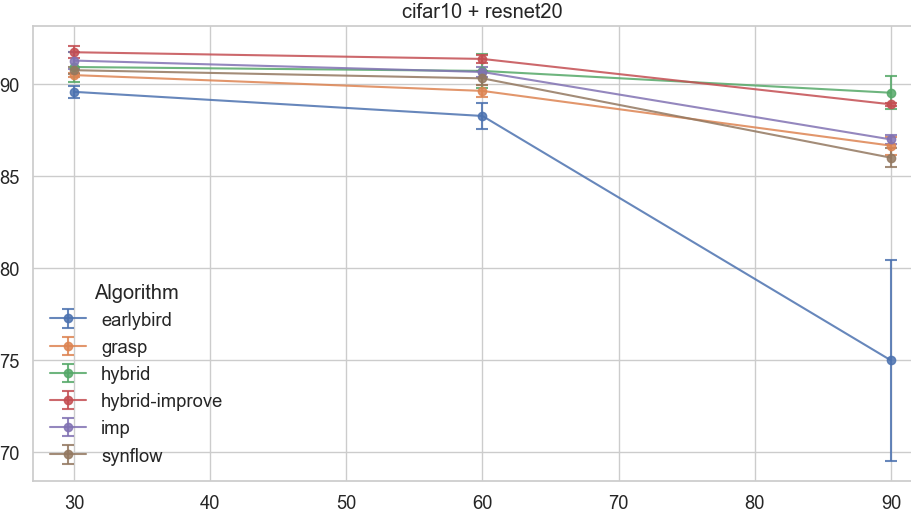
\includegraphics[width=\textwidth]{resnet20-cifar10_acc+sparsity.png}
            \caption{Độ chính xác theo mức độ thưa trên CIFAR-10/ResNet-20}
            \label{fig:resnet20-cifar10-acc-sparsity}
        \end{figure}
        Có thể thấy có 2 nhóm hành vi:
        
        \paragraph{Nhóm suy giảm từ từ:}

        GraSP, SynFlow, Hybrid, Hybrid-Improve và IMP đều duy trì độ chính xác trong khoảng
        $85\%$--$91{,}5\%$ qua tất cả các mức độ thưa.
        Tại $S=0{,}30$, Hybrid-Improve dẫn đầu ($\approx91{,}2\%$), xấp xỉ bằng mô hình gốc,
        trong khi IMP, Hybrid, GraSP và SynFlow dao động trong khoảng $90{,}0\%$--$91{,}0\%$.
        Đáng chú ý, sụt giảm của Hybrid-Improve tại $S=0{,}30$ xấp xỉ bằng không, tức là mô
        hình sau cắt tỉa nhẹ gần như tương đương mô hình gốc.
        Tại $S=0{,}90$, Hybrid và Hybrid-Improve tiếp tục dẫn đầu ($\approx89\%$--$89{,}5\%$),
        tiếp theo là GraSP và IMP ($\approx87\%$), trong khi SynFlow sụt giảm đến $\approx85\%$.

        \paragraph{Nhóm sụp đổ hiệu năng.}
        Early-Bird có hành vi hoàn toàn khác biệt.
        Ngay tại $S=0{,}30$, độ chính xác của nó ($\approx89{,}5\%$) đã thấp hơn tất cả các
        thuật toán còn lại, và tiếp tục sụt giảm mạnh: $\approx88{,}3\%$ tại $S=0{,}60$, và
        $\approx75\%$ tại $S=0{,}90$ --- mất hơn $16$ điểm phần trăm so với mô hình gốc.
        Quan trọng hơn, thanh sai số của Early-Bird tại $S=0{,}90$ là rộng nhất trong tất cả các
        thuật toán (độ lệch chuẩn $\approx5\%$--$6\%$), cho thấy hành vi của nó ở độ thưa cao
        không chỉ kém mà còn không ổn định giữa các hạt giống khác nhau.
        Nguyên nhân nằm ở bản chất của Early-Bird: điểm quan trọng kênh được tính từ hệ số
        co giãn Batch Normalisation ($\gamma$) tại các epoch rất sớm (thường $6\%$--$20\%$ tổng
        số epoch), khi mô hình chưa hội tụ. Tại $S=0{,}90$, các điểm số này quá nhiễu và nhạy
        cảm với khởi tạo khác nhau, dẫn đến việc lựa chọn kênh quan trọng sai và không nhất quán.

        \subsubsection{Sụt giảm độ chính xác}

        \begin{figure}[h]
            \centering
            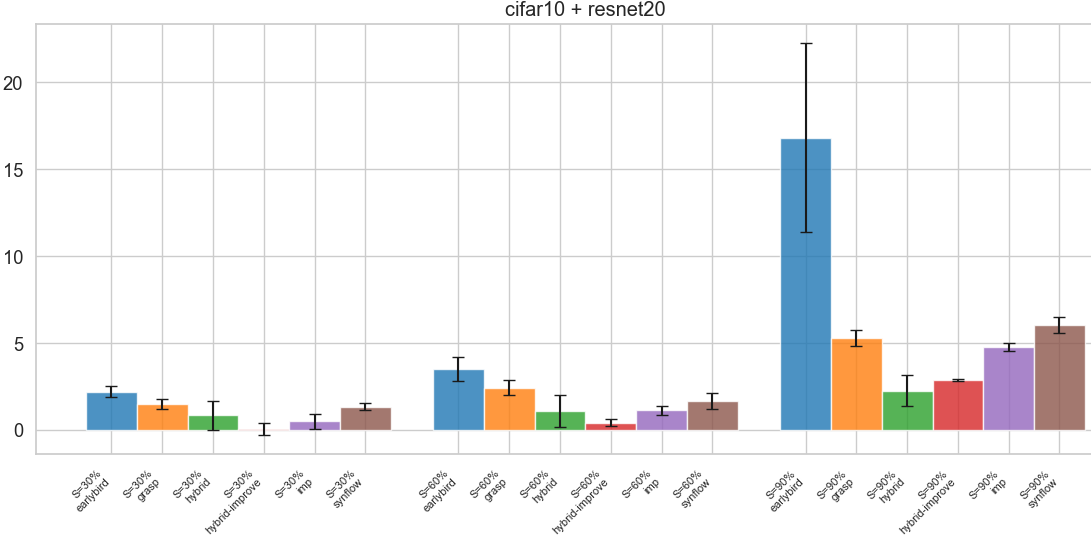
\includegraphics[width=\textwidth]{resnet20-cifar10_accdrop.png}
            \caption{Mức giảm độ chính xác so với mô hình dày đặc trên CIFAR-10/ResNet-20}
            \label{fig:resnet20-cifar10-accdrop}
        \end{figure}
        \label{subsec:r20c10_drop}
        
        Hình~\ref{fig:resnet20-cifar10-accdrop} biểu diễn sụt giảm độ chính xác trung bình và độ lệch chuẩn
        qua các hạt giống cho mỗi thuật toán tại từng mức độ thưa.
        
        Tại $S=0{,}30$, sụt giảm của tất cả các thuật toán ngoài Early-Bird đều nhỏ và tập trung:
        Hybrid-Improve $\approx0{,}0\%$, IMP $\approx0{,}5\%$, Hybrid $\approx0{,}9\%$,
        SynFlow $\approx1{,}4\%$ và GraSP $\approx1{,}5\%$.
        Thanh lỗi nhỏ ở mức này xác nhận rằng $S=0{,}30$ nằm trong vùng nén an toàn cho
        ResNet-20 với tất cả các phương pháp không có cấu trúc.
        
        Tại $S=0{,}60$, thứ hạng được giữ nguyên: Hybrid-Improve vẫn dẫn đầu ($\approx0{,}5\%$),
        tiếp theo là Hybrid ($\approx1{,}1\%$), IMP ($\approx1{,}3\%$), SynFlow ($\approx1{,}7\%$)
        và GraSP ($\approx2{,}4\%$).
        
        Điều quan trọng nhất nằm ở $S=0{,}90$.
        Early-Bird đạt sụt giảm trung bình $\approx17\%$ với độ lệch chuẩn $\approx6\%$ --- một
        mức biến động cực kỳ cao, có nghĩa là trong điều kiện tệ nhất, mô hình có thể mất hơn
        $23\%$ độ chính xác.
        Trong số các phương pháp còn lại, Hybrid dẫn đầu với chỉ $\approx2{,}2\%$ sụt giảm,
        tiếp theo là Hybrid-Improve ($\approx3{,}0\%$), IMP ($\approx5{,}0\%$), GraSP
        ($\approx5{,}5\%$) và SynFlow ($\approx6{,}2\%$).
        
        Đáng chú ý, Hybrid ở $S=0{,}90$ vượt qua Hybrid-Improve theo
        giá trị trung bình. Tuy nhiên, biên độ độ chính xác của Hybrid lớn hơn đáng kể so với 
        Hybrid-Improve, do đó vẫn có thể nói rằng Hybrid-Improve có hiệu suất ổn định hơn ở mức độ thưa cực cao.
        \subsubsection{Mức giảm FLOPs vs chi phí huấn luyện và độ chính xác}
        \label{subsec:r20c10_efficiency}
        \noindent
        \begin{figure}[h]
            \centering
            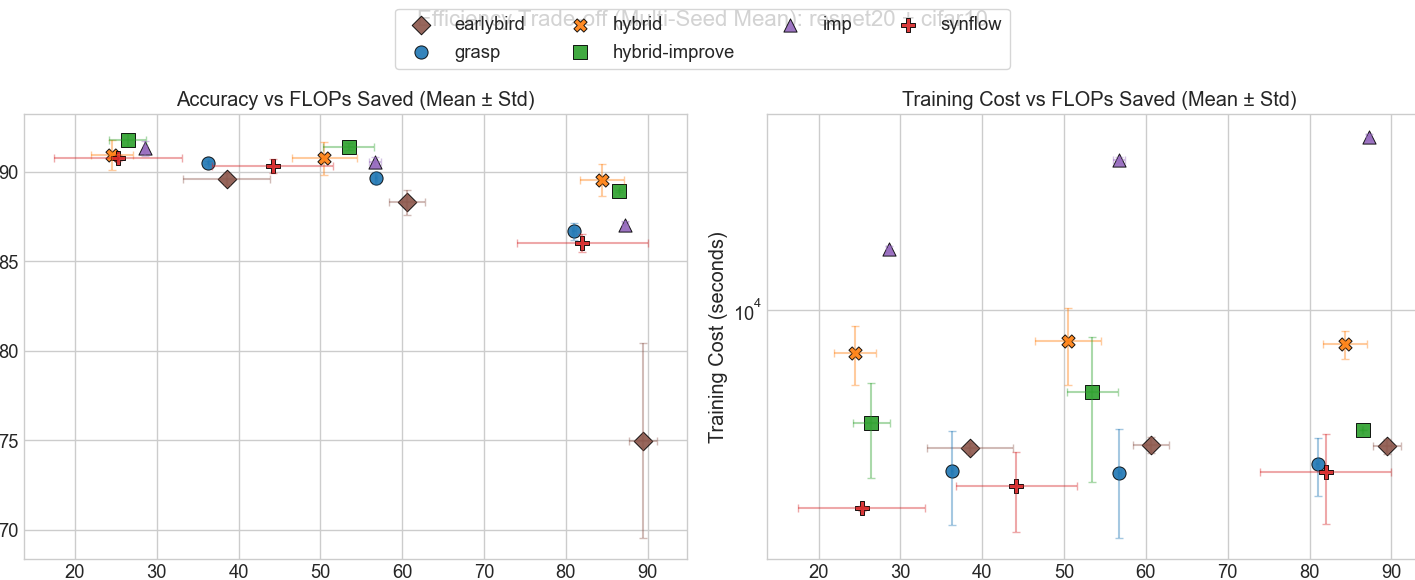
\includegraphics[width=\textwidth]{resnet20-cifar10_pareto.png}
            \caption{Biểu đồ Pareto: Cân bằng giữa độ chính xác và độ trễ trên CIFAR-10/ResNet-20}
            \label{fig:resnet20-cifar10-pareto}
        \end{figure}

        Hình~\ref{fig:resnet20-cifar10-pareto} trình bày hai biểu đồ phân tán: (trái) độ chính xác so
        với mức giảm FLOPs tiết kiệm, và (phải) chi phí huấn luyện so với mức giảm FLOPs.
        Cả hai đều hiển thị giá trị trung bình và thanh lỗi qua nhiều hạt giống.
        
        Cần lưu ý rằng mức giảm FLOPs được ước lượng theo mật độ mặt nạ và là các giá trị lý thuyết, không phải phép đo phần
        cứng thực tế.
        
        Tại tỉ lệ giảm FLOPs $\approx20\%$--$50\%$, GraSP, Hybrid và Hybrid-Improve
        tập trung gần phía trên của trục độ chính xác ($\approx90\%$--$91\%$), cho thấy chúng
        là các phương pháp hiệu quả nhất khi nén nhẹ.
        Ở tỉ lệ giảm FLOPs $>80\%$, Hybrid và Hybrid-Improve
        nằm trên biên Pareto với $\approx89\%$--$89{,}5\%$, tiếp theo là GraSP và IMP ở
        $\approx87\%$.
        
        Về chi phí huấn luyện, IMP là đắt nhất ở mọi mức độ thưa ($10^4$--$10^5$ giây), do có
        nhiều vòng prune-retrain-rewind. Hybrid và Hybrid-Improve ở mức trung gian, trong khi
        GraSP và SynFlow rẻ nhất vì chỉ cần 1 lần cắt tỉa và một lần huấn luyện.
        Tuy nhiên, kết quả cho thấy IMP có biến động chi phí thấp,
        trong khi Hybrid và Hybrid-Improve có biến động vừa phải tùy thuộc vào khi nào \gls{early_stopping} được kích hoạt. % original hybrid paper suggests this

        \subsubsection{Phân phối độ thưa theo tầng và tính ổn định}
        \label{subsec:r20c10_layerwise}

        \begin{figure}[h]
            \centering
            \begin{subfigure}{0.49\textwidth}
                \centering
                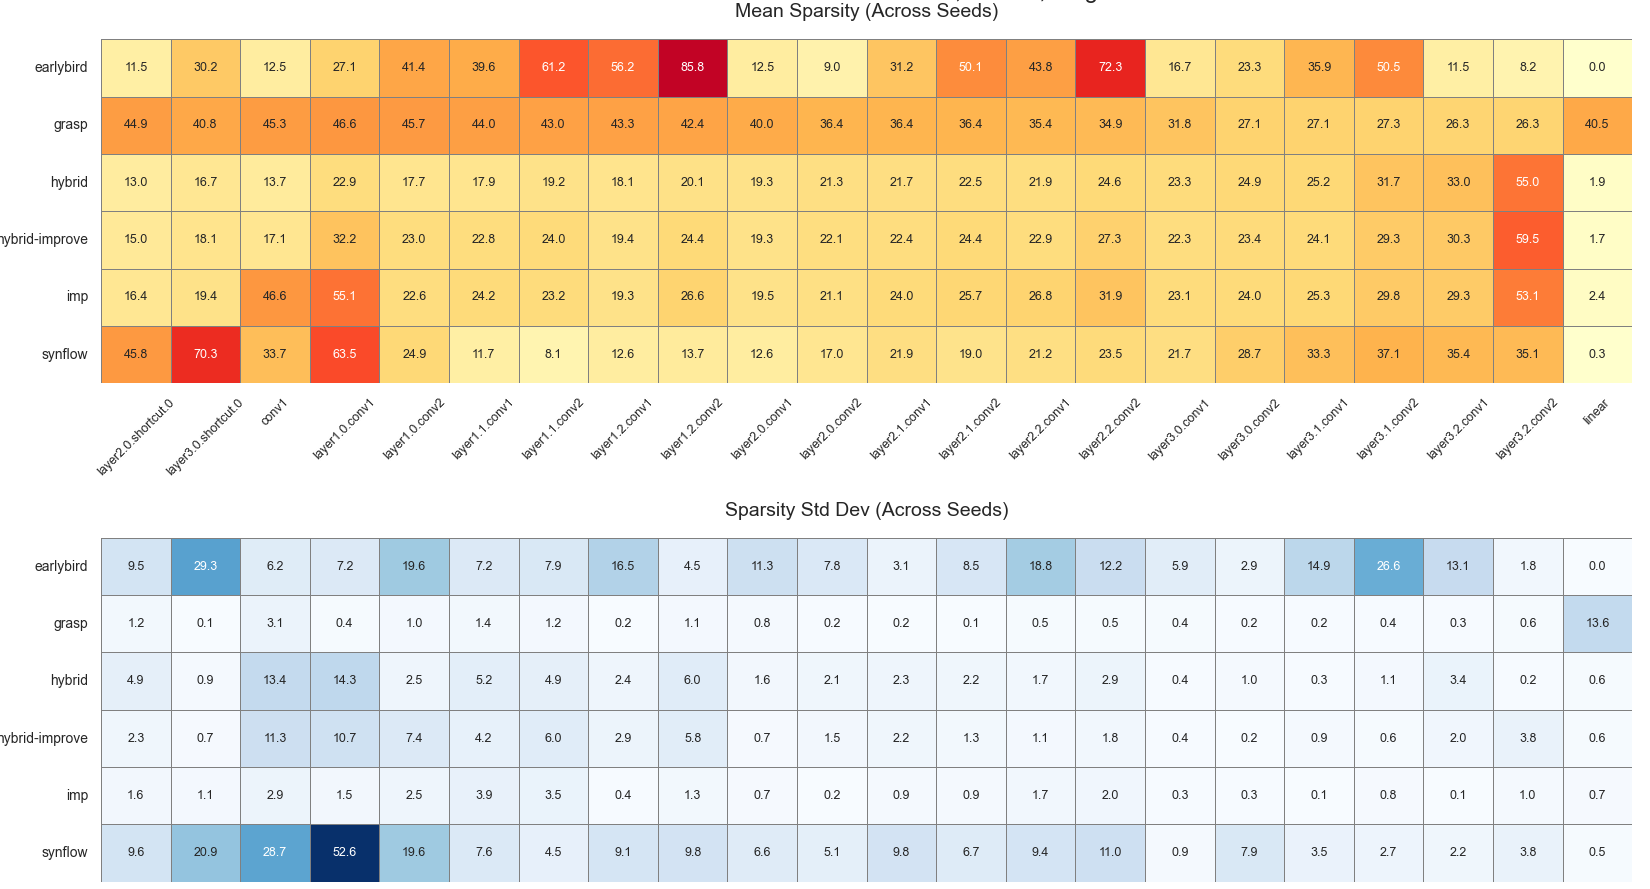
\includegraphics[width=\textwidth]{resnet20-cifar10_s0.3_heatmap.png}
                \caption{Bản đồ nhiệt phân phối độ thưa theo tầng tại $S=0{,}30$}
                \label{fig:r20c10_heatmap_s03}
            \end{subfigure}
            \hfill
            \begin{subfigure}{0.49\textwidth}
                \centering
                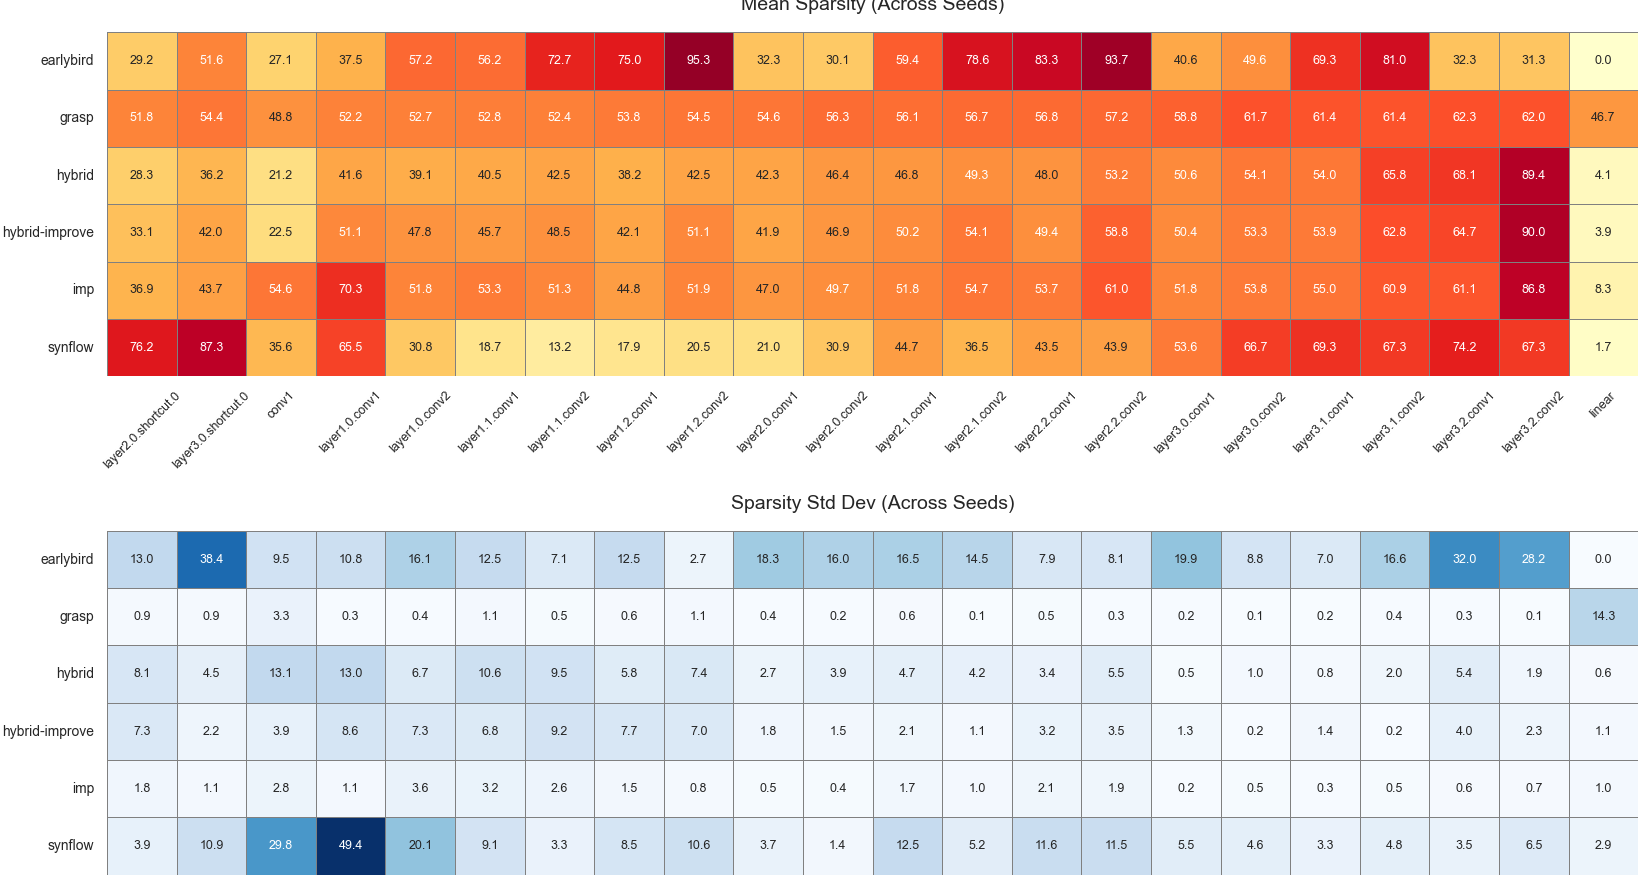
\includegraphics[width=\textwidth]{resnet20-cifar10_s0.6_heatmap.png}
                \caption{Bản đồ nhiệt phân phối độ thưa theo tầng tại $S=0{,}60$}
                \label{fig:r20c10_heatmap_s06}
            \end{subfigure}
            \hfill
            \begin{subfigure}{0.49\textwidth}
                \centering
                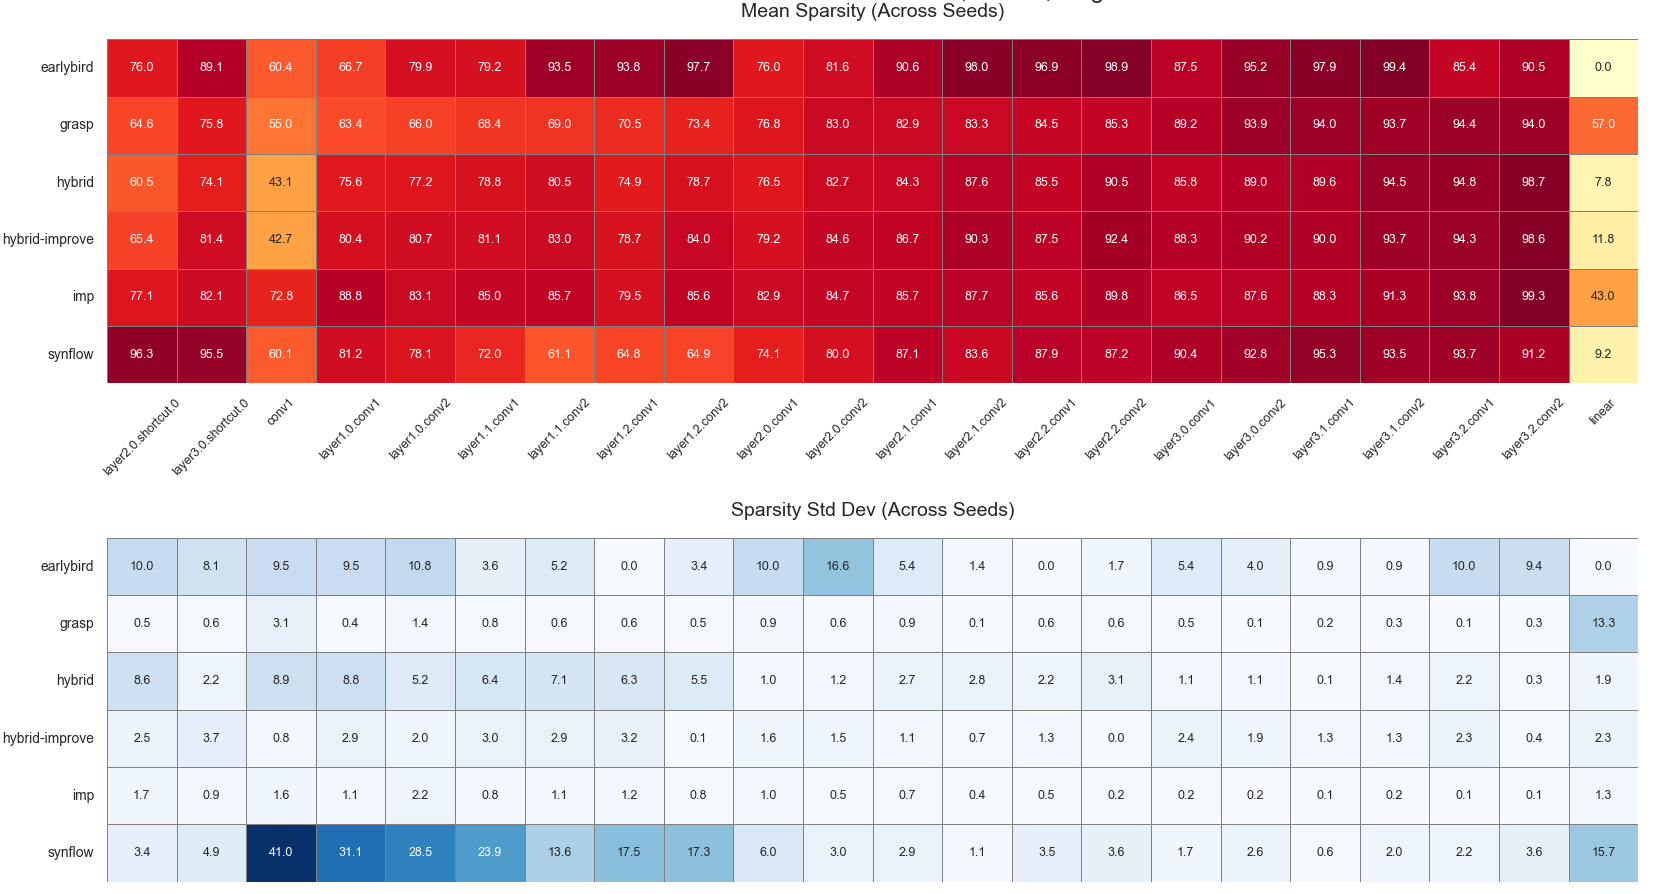
\includegraphics[width=\textwidth]{resnet20-cifar10_s0.9_heatmap.png}
                \caption{Bản đồ nhiệt phân phối độ thưa theo tầng tại $S=0{,}90$}
                \label{fig:r20c10_heatmap_s09}
            \end{subfigure}

            \caption{Bản đồ nhiệt phân phối độ thưa theo tầng trên CIFAR-10/ResNet-20}
            \label{fig:grouped-accuracy}
        \end{figure}
        
        Hình~\ref{fig:r20c10_heatmap_s03}, \ref{fig:r20c10_heatmap_s06} và
        \ref{fig:r20c10_heatmap_s09} hiển thị cả bản đồ nhiệt trung bình và
        độ lệch chuẩn của phân phối độ thưa theo tầng qua các cài đặt.
        
        GraSP cho thấy phân phối độ thưa đồng đều nhất qua tất cả các tầng ở cả ba mức độ thưa,
        với độ lệch chuẩn rất thấp trên hầu hết các tầng.
        Tính đồng đều trong phân phối của GraSP là hệ quả trực tiếp từ tiêu chí bảo toàn chuẩn gradient: vì chuẩn gradient
        phụ thuộc vào luồng thông tin qua toàn bộ mạng, bất kỳ tầng nào bị cắt tỉa quá mạnh đều tạo ra
        nút thắt cổ chai làm giảm gradient toàn cục, khiến các trọng số tại tầng đó nhận điểm saliency
        cao và được bảo vệ, điều này tự nhiên khuyến khích cắt tỉa đồng đều trên tất cả các tầng.
        
        IMP cũng có độ lệch chuẩn rất thấp qua các tầng, điều này có thể giải thích bởi tính xác định
        cao của tiêu chí magnitude sau huấn luyện đầy đủ — các trọng số hội tụ về vùng tương tự qua
        các hạt giống, dẫn đến ngưỡng cắt tỉa toàn cục nhất quán. % Morcos et al. (2019) "One ticket to win them all" cho thấy winning ticket có thể transfer qua datasets
        Tuy nhiên, IMP tập trung độ thưa cao hơn vào các tầng đầu (ví dụ
        \texttt{layer1.0.conv1}: $55{,}1\%$ tại $S=0{,}30$), Điều này có thể giải thích do
        các tầng đầu của ResNet-20 trên CIFAR-10 thường học các đặc trưng mức thấp như cạnh
        và kết cấu đơn giản, do đó có thể chứa nhiều trọng số dư thừa hoặc có độ lớn nhỏ. Vì
        vậy, các tầng này thường bị cắt tỉa mạnh hơn.
        Cả hai biến thể hybrid đều thể hiện xu hướng bảo vệ tầng đầu: tầng \texttt{conv1}
        chỉ đạt $\approx13\%$--$17\%$ độ thưa tại $S=0{,}30$, trong khi các tầng sâu hơn nhận
        được cắt tỉa nhiều hơn (ví dụ \texttt{layer3.2.conv2}: $55\%$--$59{,}5\%$).
        Độ lệch chuẩn ở mức trung bình --- 
        phản ánh sự kết hợp của hai giai đoạn cắt tỉa một lần và lặp. 

        SynFlow là thuật toán kém ổn định nhất trong số các phương pháp được đánh giá.
        Tại $S=0{,}30$, độ lệch chuẩn đạt tới $52{,}6\%$ tại \texttt{layer1.0.conv1} và $28{,}7\%$
        tại \texttt{conv1}. Điều này có nghĩa là quyết định phân bổ độ thưa cho các tầng quan
        trọng này thay đổi rất lớn giữa các hạt giống.
        Nguyên nhân nằm ở tính nhạy cảm của điểm SynFlow đối với giá trị khởi tạo ngẫu nhiên:
        vì điểm path-norm được tính tại thời điểm khởi tạo mà không dùng dữ liệu thực, các trọng % 
        số được khởi tạo khác nhau sẽ tạo ra phân phối điểm rất khác nhau.
        Sự không ổn định trong phân phối độ thưa theo tầng trực tiếp giải thích sự biến động cao
        trong độ chính xác cuối cùng của SynFlow qua các hạt giống.
        
        Bản đồ độ lệch chuẩn của Early-Bird cho thấy biến động lớn ở nhiều tầng, đặc biệt ở các
        kết nối shortcut và các tầng conv đầu (ví dụ \texttt{layer3.0.shortcut.0}: $\sigma=26{,}6\%$ % wrong data
        tại $S=0{,}30$).
        Điều này xác nhận rằng các điểm quan trọng kênh dựa trên hệ số $\gamma$ BN ở giai đoạn
        huấn luyện sớm không ổn định và phụ thuộc nhiều vào hạt giống khởi tạo, dẫn đến các quyết
        định cắt tỉa cấu trúc khác nhau và do đó độ chính xác khác nhau đáng kể giữa các lần chạy


        \subsection{CIFAR-100/ResNet-20}

        CIFAR-100 là bộ dữ liệu khó hơn đáng kể so với CIFAR-10: $100$ lớp thay vì $10$ lớp,
        với $600$ ảnh mỗi lớp thay vì $6000$, đòi hỏi mô hình phải học các đặc trưng phân biệt
        tinh tế hơn với ít dữ liệu huấn luyện hơn mỗi lớp.
        Khi áp dụng cùng các thuật toán cắt tỉa trên cấu hình ResNet-20/CIFAR-100, tác động của cắt tỉa sẽ nghiêm trọng hơn, đặc biệt ở mức độ thưa cao, vì mạng cần
        duy trì khả năng phân biệt giữa nhiều lớp hơn với ít tham số hơn.
        
        \subsubsection{Độ chính xác và sụt giảm theo mức độ thưa}
        \label{subsec:r20c100_acc}

        \begin{figure}[h]
            \centering

            \begin{subfigure}{0.49\textwidth}
                \centering
                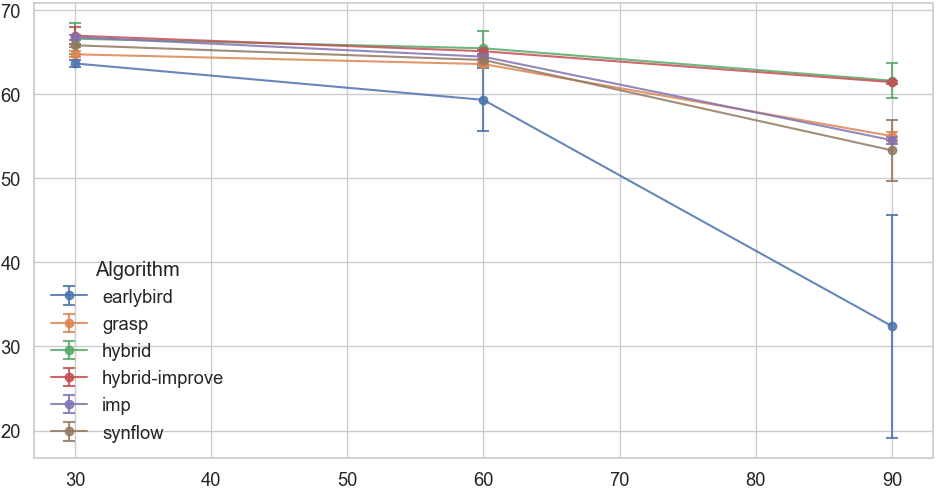
\includegraphics[width=\textwidth]{resnet20-cifar100_acc+sparsity.png}
                \caption{Độ chính xác theo mức độ thưa trên CIFAR-100/ResNet-20}
                \label{fig:resnet20-cifar100-acc-sparsity}
            \end{subfigure}
            \hfill
            \begin{subfigure}{0.49\textwidth}
                \centering
                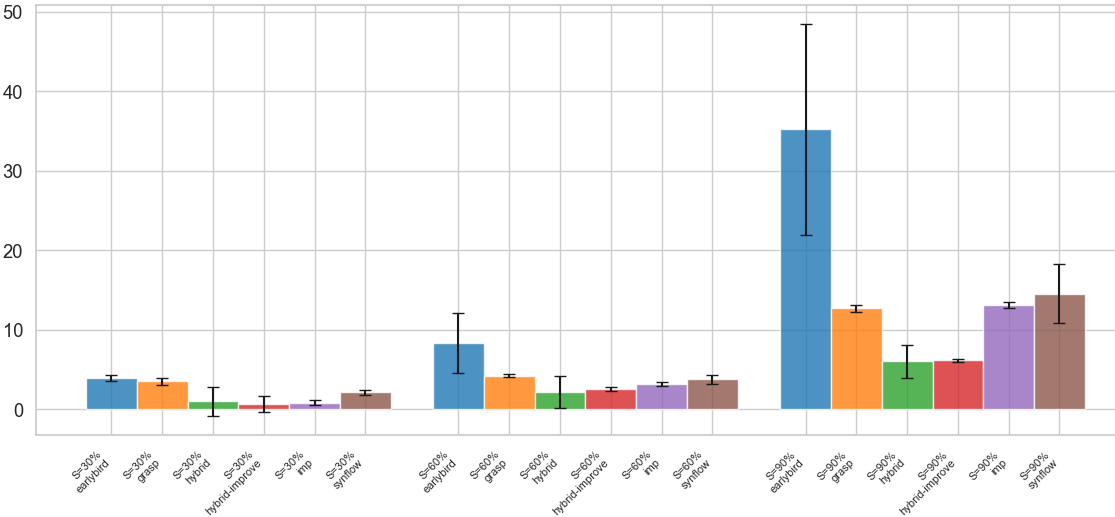
\includegraphics[width=\textwidth]{resnet20-cifar100_accdrop.png}
                \caption{Mức giảm độ chính xác so với mô hình dày đặc trên CIFAR-100/ResNet-20}
                \label{fig:resnet20-cifar100-accdrop}
            \end{subfigure}

            \caption{Độ chính xác theo mức độ thưa trên CIFAR-100/ResNet-20}
            \label{fig:grouped-accuracy}
        \end{figure}
        
        Hình~\ref{fig:resnet20-cifar100-acc-sparsity} và \ref{fig:resnet20-cifar100-accdrop} cho thấy xu hướng tương tự như
        CIFAR-10 nhưng với mức sụt giảm lớn hơn đáng kể.
        
        Tại $S=0{,}30$, Hybrid và Hybrid-Improve gần như không sụt giảm ($\approx1{,}0\%$ và
        $\approx0{,}7\%$ tương ứng), trong khi IMP sụt giảm $\approx0{,}7\%$, SynFlow $\approx2{,}5\%$,
        GraSP và Early-Bird cùng $\approx3{,}8\%$.
        Thanh lỗi nhỏ cho hầu hết các thuật toán ở mức này cho thấy $S=0{,}30$ vẫn trong vùng
        nén an toàn trên CIFAR-100 với các phương pháp không có cấu trúc.
        
        Tại $S=0{,}60$, khoảng cách giữa các thuật toán bắt đầu mở rộng rõ rệt.
        Early-Bird sụt giảm $\approx8{,}5\%$ với thanh lỗi lớn, cho thấy độ không ổn định đặc
        trưng của nó.
        Hybrid ($\approx2{,}2\%$) và Hybrid-Improve ($\approx2{,}5\%$) vẫn duy trì hiệu suất tốt.
        GraSP ($\approx4\%$), IMP ($\approx3\%$) và SynFlow ($\approx4\%$) ở mức trung gian.
        
        Tại $S=0{,}90$, sự phân hóa trở nên cực kỳ rõ ràng:
        \begin{itemize}
            \item \textbf{Early-Bird:} sụt giảm trung bình $\approx35\%$ với độ lệch chuẩn lên
            đến $\approx13\%$. Trong điều kiện tệ nhất (mean + 1 std), độ chính xác có thể rơi
            xuống dưới $20\%$ --- gần như không thể sử dụng được. Đây là hành vi sụp đổ nghiêm
            trọng nhất trong toàn bộ thực nghiệm.
            \item \textbf{GraSP và IMP:} cùng sụt giảm $\approx13\%$ --- lớn hơn gấp đôi so với
            CIFAR-10 ở cùng mức độ thưa.
            \item \textbf{SynFlow:} sụt giảm $\approx14{,}5\%$ --- lớn hơn đáng kể so với CIFAR-10
            ($\approx6{,}2\%$).
            \item \textbf{Hybrid và Hybrid-Improve:} cùng sụt giảm $\approx6\%$, dẫn đầu so với các
            thuật toán khác với biên độ tương đối nhỏ.
        \end{itemize}
        
        Việc mức sụt giảm lớn hơn đối với GraSP, IMP và SynFlow trên CIFAR-100 là có thể dự đoán được.
        Trên CIFAR-100, mỗi tham số mang nhiều thông tin phân loại hơn
        do phải phân biệt $10\times$ nhiều lớp hơn với $10\times$ ít dữ liệu hơn mỗi lớp hơn so với CIFAR-10.
        Cắt tỉa $90\%$ tham số do đó loại bỏ nhiều thông tin không thể phục hồi hơn, và khả năng
        phục hồi thông qua tinh chỉnh bị hạn chế hơn vì tập dữ liệu nhỏ hơn theo lớp.
        Các biến thể hybrid vẫn vượt trội nhờ chiến lược phân giai đoạn: cắt tỉa từ từ và tinh
        chỉnh với kiên nhẫn sau mỗi bước đặc biệt quan trọng khi tập dữ liệu nhỏ hơn theo lớp,
        vì mô hình cần nhiều epoch hơn để hội tụ lại sau mỗi bước cắt tỉa.
        
        \subsubsection{Phân phối độ thưa theo tầng và tính ổn định}
        \label{subsec:r20c100_layerwise}

        \begin{figure}[h]
            \centering
            \begin{subfigure}{0.49\textwidth}
                \centering
                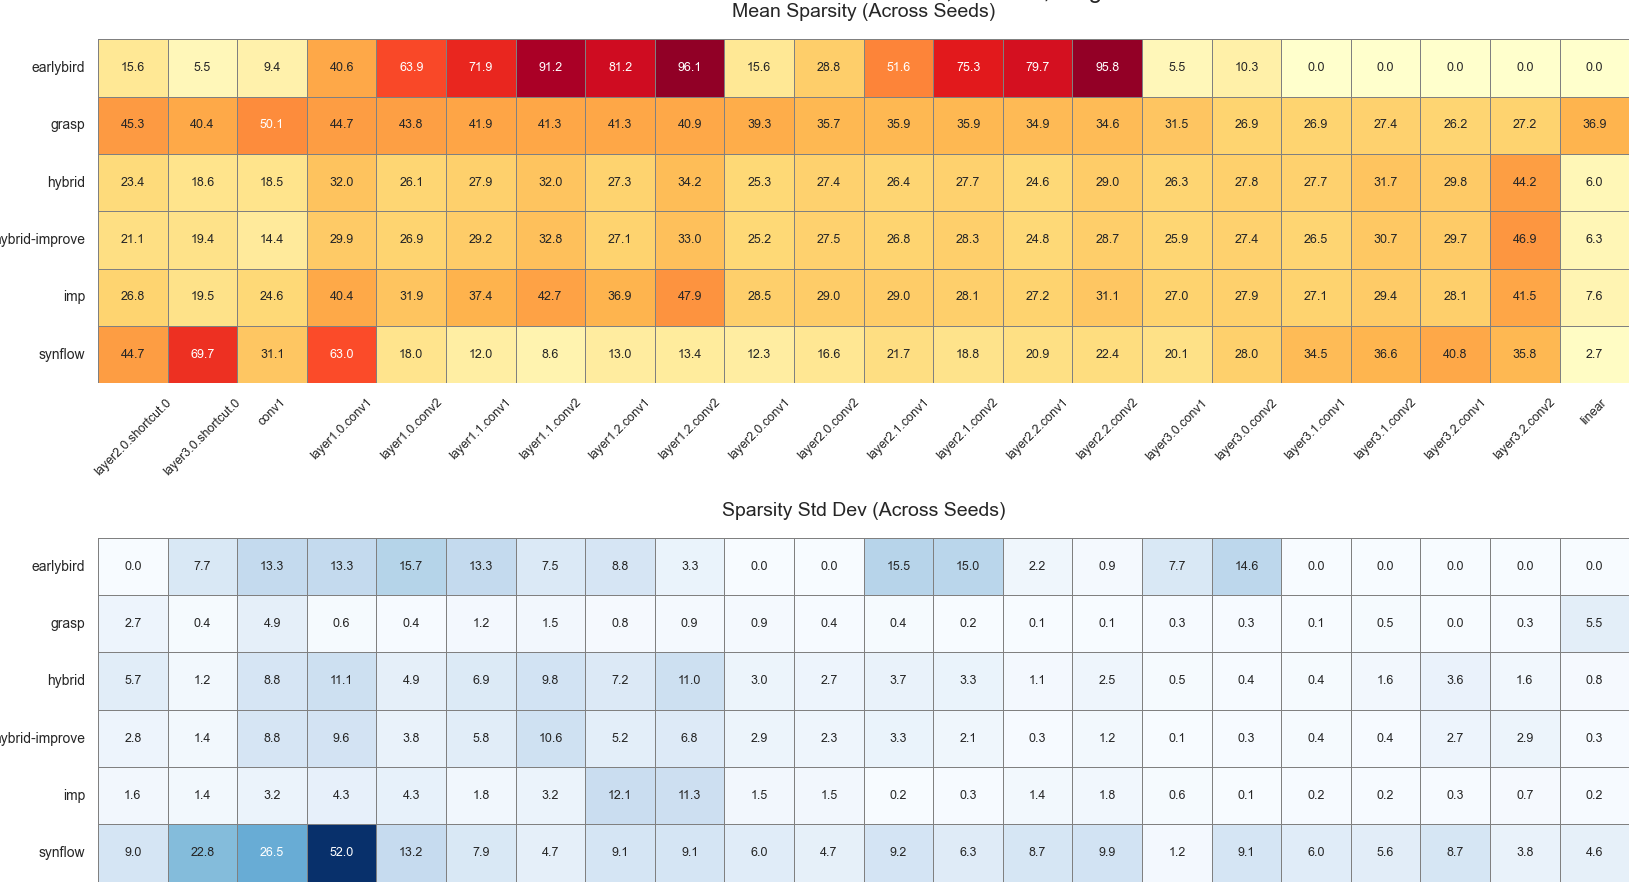
\includegraphics[width=\textwidth]{resnet20-cifar100_s0.3_heatmap.png}
                \caption{Bản đồ nhiệt phân phối độ thưa theo tầng tại $S=0{,}30$}
                \label{fig:r20c100_heatmap_s03}
            \end{subfigure}
            \hfill
            \begin{subfigure}{0.49\textwidth}
                \centering
                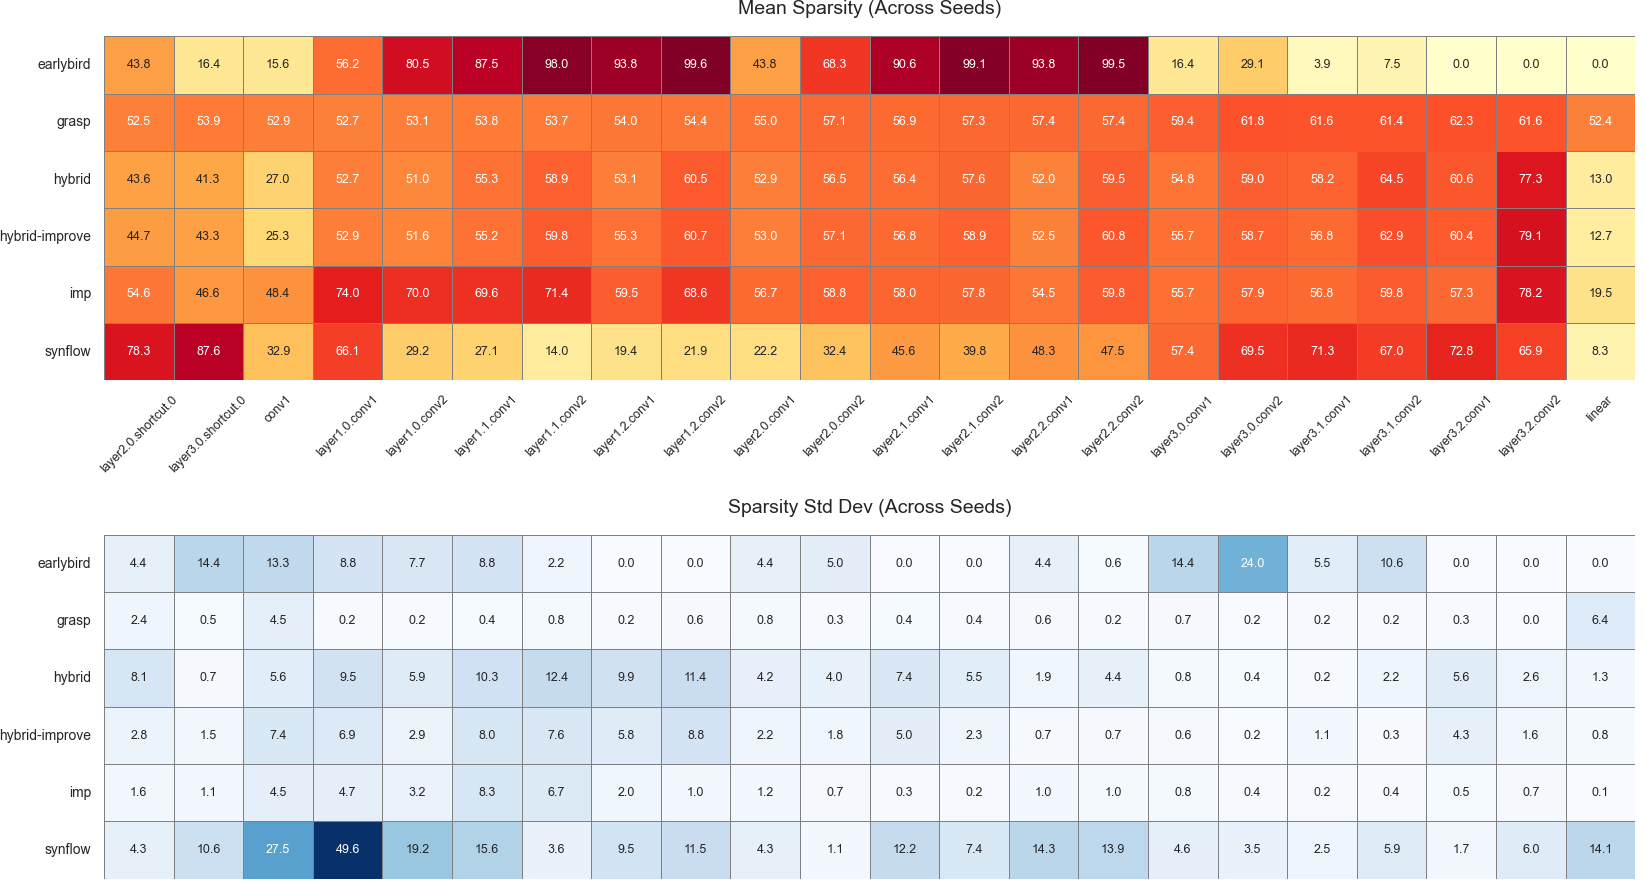
\includegraphics[width=\textwidth]{resnet20-cifar100_s0.6_heatmap.png}
                \caption{Bản đồ nhiệt phân phối độ thưa theo tầng tại $S=0{,}60$}
                \label{fig:r20c100_heatmap_s06}
            \end{subfigure}
            \hfill
            \begin{subfigure}{0.49\textwidth}
                \centering
                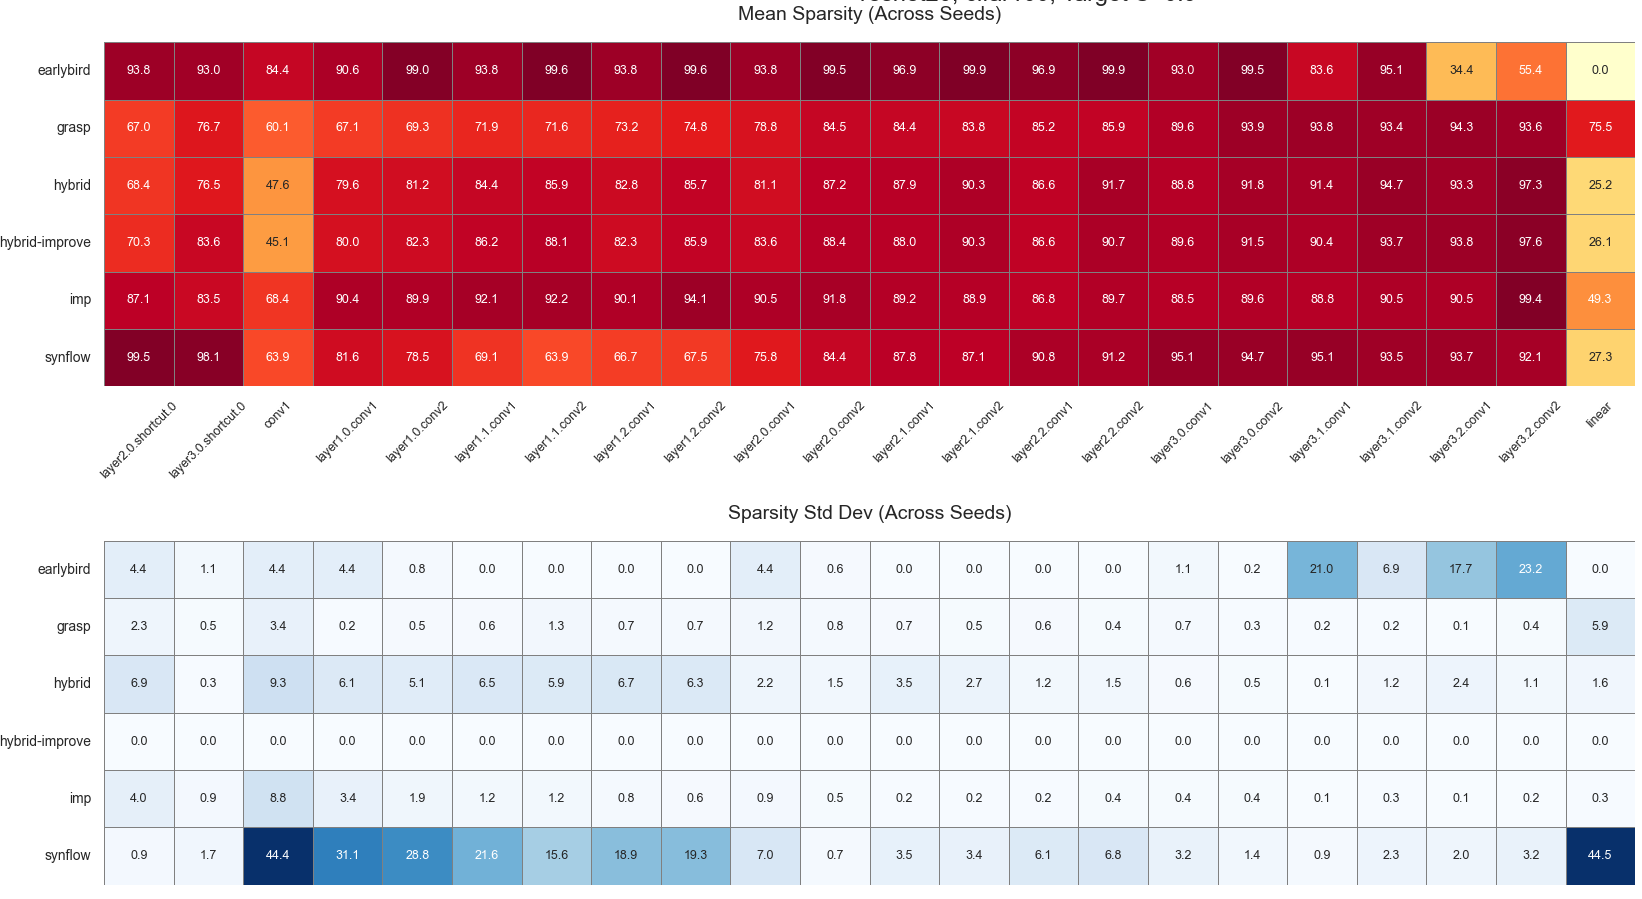
\includegraphics[width=\textwidth]{resnet20-cifar100_s0.9_heatmap.png}
                \caption{Bản đồ nhiệt phân phối độ thưa theo tầng tại $S=0{,}90$}
                \label{fig:r20c100_heatmap_s09}
            \end{subfigure}

            \caption{Bản đồ nhiệt phân phối độ thưa theo tầng trên CIFAR-100/ResNet-20}
            \label{fig:grouped-accuracy}
        \end{figure}
        
        Hình~\ref{fig:r20c100_heatmap_s03}, \ref{fig:r20c100_heatmap_s06} và
        \ref{fig:r20c100_heatmap_s09} cho thấy các xu hướng phân phối tương tự như CIFAR-10 nhưng
        với một số điểm khác biệt đáng chú ý.

        Early-Bird trên CIFAR-100 tại $S=0{,}30$ đã có nhiều tầng đạt $>90\%$ độ thưa kênh
        (ví dụ \texttt{layer1.2.conv2}: $96{,}1\%$; \texttt{layer3.0.shortcut.0}: $95{,}8\%$),
        sớm và cực đoan hơn nhiều so với CIFAR-10.
        Điều này cho thấy điểm $\gamma$ BN trên CIFAR-100 tạo ra phân phối thưa kênh nghiêm trọng
        hơn ngay cả ở mức nén nhẹ --- một phần vì mô hình trên CIFAR-100 học được ít kênh ``dư
        thừa'' hơn, khiến các điểm $\gamma$ phân biệt rõ hơn và dẫn đến cắt tỉa hung hăng hơn.
        
        SynFlow trên CIFAR-100 duy trì mô hình độ lệch chuẩn cao ở các tầng đầu
        (\texttt{conv1}: $\sigma=26{,}5\%$; \texttt{layer1.0.conv1}: $\sigma=52{,}0\%$ tại $S=0{,}30$),
        xác nhận rằng sự không ổn định của SynFlow là đặc trưng của phương pháp chứ không phải
        của bộ dữ liệu cụ thể.
        
        \subsubsection{Mức giảm FLOPs vs chi phí huấn luyện và độ chính xác}
        \label{subsec:r20c100_efficiency}

        \begin{figure}[h]
            \centering
            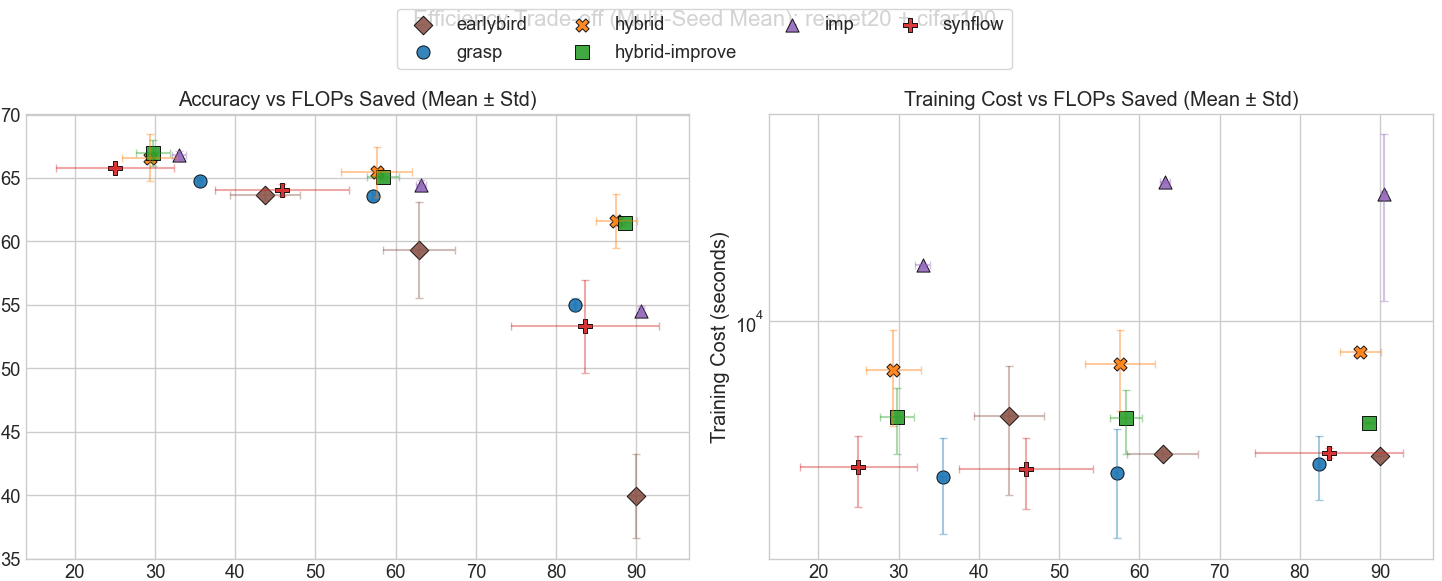
\includegraphics[width=\textwidth]{resnet20-cifar100_pareto.png}
            \caption{Biểu đồ Pareto: Cân bằng giữa độ chính xác và độ trễ trên CIFAR-100/ResNet-20}
            \label{fig:resnet20-cifar100-pareto}
        \end{figure}
        
        Hình~\ref{fig:resnet20-cifar100-pareto} cho thấy bức tranh hiệu quả tương tự như CIFAR-10 nhưng
        với dải độ chính xác thấp hơn ($35\%$--$67\%$ thay vì $75\%$--$91\%$).
        
        Tại tỉ lệ giảm FLOPs cao ($>80\%$), Hybrid và Hybrid-Improve đạt $\approx61{,}5\%$ độ chính
        xác với chi phí huấn luyện trung bình, trong khi GraSP đạt $\approx55\%$ với chi phí thấp
        hơn đáng kể.
        IMP đạt $\approx54{,}5\%$ với chi phí rất cao --- càng khẳng định rằng chi phí
        cao của IMP không tương xứng với hiệu suất ở mức độ thưa cực cao.
        SynFlow đạt $\approx53\%$ với chi phí thấp, nhưng với độ biến động cao hơn.

        \subsection{CIFAR-10/ResNet-50}

        \subsubsection{Độ chính xác và sụt giảm theo mức độ thưa}
        \label{subsec:r50_acc}
        \begin{figure}
            \centering
            \begin{subfigure}{0.49\textwidth}
                \centering
                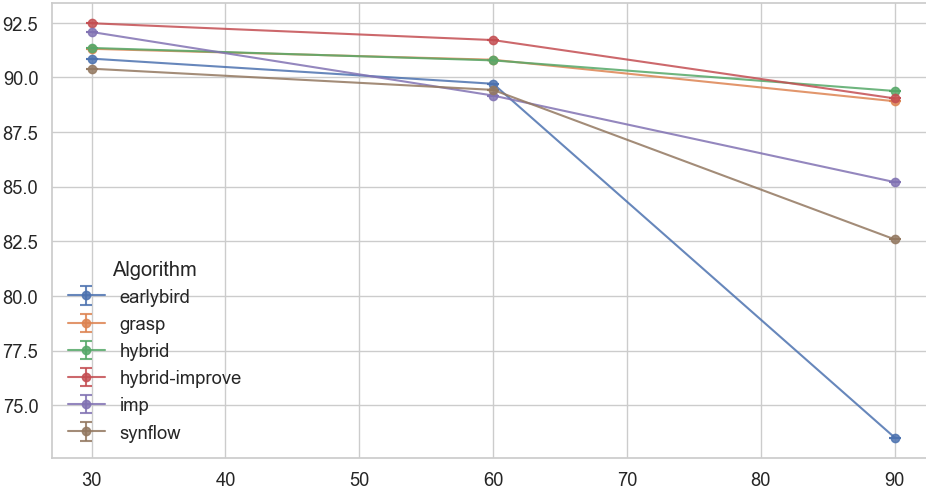
\includegraphics[width=\textwidth]{resnet50-cifar10_acc+sparsity.png}
                \caption{Độ chính xác theo mức độ thưa trên CIFAR-10/ResNet-50}
                \label{fig:resnet50-cifar10-acc-sparsity}
            \end{subfigure}
            \hfill
            \begin{subfigure}{0.49\textwidth}
                \centering
                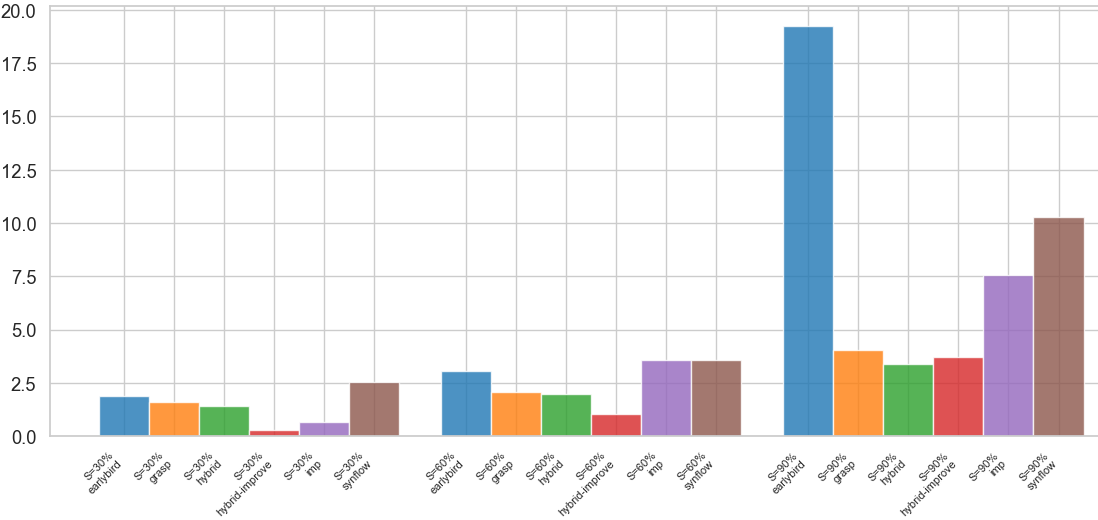
\includegraphics[width=\textwidth]{resnet50-cifar10_accdrop.png}
                \caption{Mức giảm độ chính xác so với mô hình dày đặc trên CIFAR-10/ResNet-50}
                \label{fig:resnet50-cifar10-accdrop}
            \end{subfigure}

            \caption{Độ chính xác theo mức độ thưa trên CIFAR-10/ResNet-50}
            \label{fig:grouped-accuracy}
        \end{figure}
        
        Hình~\ref{fig:resnet50-cifar10-acc-sparsity} và \ref{fig:resnet50-cifar10-accdrop} cho thấy các hiện tượng sau:

        Sụt giảm âm $\approx-0{,}3\%$ của Hybrid-Improve tại $S=0{,}30$ không phải là sai số
        đo lường --- đây là hiệu ứng điều chỉnh ngầm trong vùng dư thừa tham số, nơi cắt tỉa
        nhẹ loại bỏ nhiễu và cải thiện khả năng tổng quát hóa.
        Hybrid cũng đạt sụt giảm thấp ($\approx1{,}4\%$).
        
        Hybrid-Improve tiếp tục dẫn đầu ($\approx1\%$ sụt giảm), tiếp theo là Hybrid
        ($\approx2\%$), GraSP ($\approx2\%$), Early-Bird ($\approx3\%$), IMP ($\approx3{,}5\%$)
        và SynFlow ($\approx3{,}5\%$).
        Sự nhất quán qua các kiến trúc củng cố kết luận rằng chiến lược hybrid mạnh mẽ ở mức nén
        vừa phải bất kể độ sâu mạng.
        
        Sụt giảm của IMP tăng từ $\approx5\%$ trên ResNet-20 lên $\approx7{,}5\%$ trên ResNet-50,
        trong khi cấu hình ($10$ vòng lặp, $160$ epoch/vòng) không được tinh chỉnh lại.
        Trên ResNet-50 ($\approx25$M tham số), $10$ vòng lặp phải xử lý không gian trọng số phức
        tạp hơn nhiều, và điều kiện ổn định cần thiết cho cơ chế rewind khó đạt được hơn trong
        cùng số epoch.
        
        Sụt giảm của SynFlow tăng từ $\approx6{,}2\%$ trên ResNet-20 lên $\approx10{,}5\%$ ---
        mức tăng lớn nhất trong tất cả các thuật toán không phải Early-Bird.
        Như được ghi nhận trong bản đồ nhiệt (Hình~\ref{fig:r50_heatmap_s09}), tại $S=0{,}90$
        nhiều tầng shortcut đạt $\approx100\%$ độ thưa, loại bỏ hiệu quả các kết nối residual và
        biến ResNet-50 thành một mạng phẳng bị hư hại nghiêm trọng.
        ResNet-50 có nhiều bottleneck block hơn gấp ba lần ResNet-20, mỗi block có một shortcut
        chiếu $1{\times}1$, làm trầm trọng thêm xu hướng của SynFlow khi tập trung độ thưa vào các
        kết nối này.
        
        Hybrid đạt $\approx3{,}3\%$ sụt giảm độ chính xác tại $S=0{,}90$ trên ResNet-50 --- tốt hơn so với
        ResNet-20.
        Hybrid-Improve đạt $\approx3{,}5\%$ --- hầu như không đổi so với ResNet-20.
        Sự ổn định giữa các kiến trúc này là kết quả quan trọng: chiến lược cắt tỉa của 2 thuật toán này không  
        có bước reset weight như IMP (cũng sử dụng magnitude như tiêu chí cắt tỉa) cho phép mạng thích nghi dần
        thay vì phải học lại từ đầu sau mỗi vòng như IMP.

        Early-Bird sụt giảm ~19\% trên ResNet-50, tệ hơn so với ~17\% trên ResNet-20,
        mặc dù ResNet-50 có kênh rộng hơn cung cấp nhiều
        dư địa hơn trước. Hành vi sụp đổ vẫn xảy ra do điểm $\gamma$ BN tại giai đoạn sớm 
        không đủ tin cậy ở $S=0{,}90$.
        
        \subsubsection{Phân phối độ thưa theo tầng và tính ổn định}
        \label{subsec:r50_layerwise}

        \begin{figure}[h]
            \centering
            \begin{subfigure}{0.49\textwidth}
                \centering
                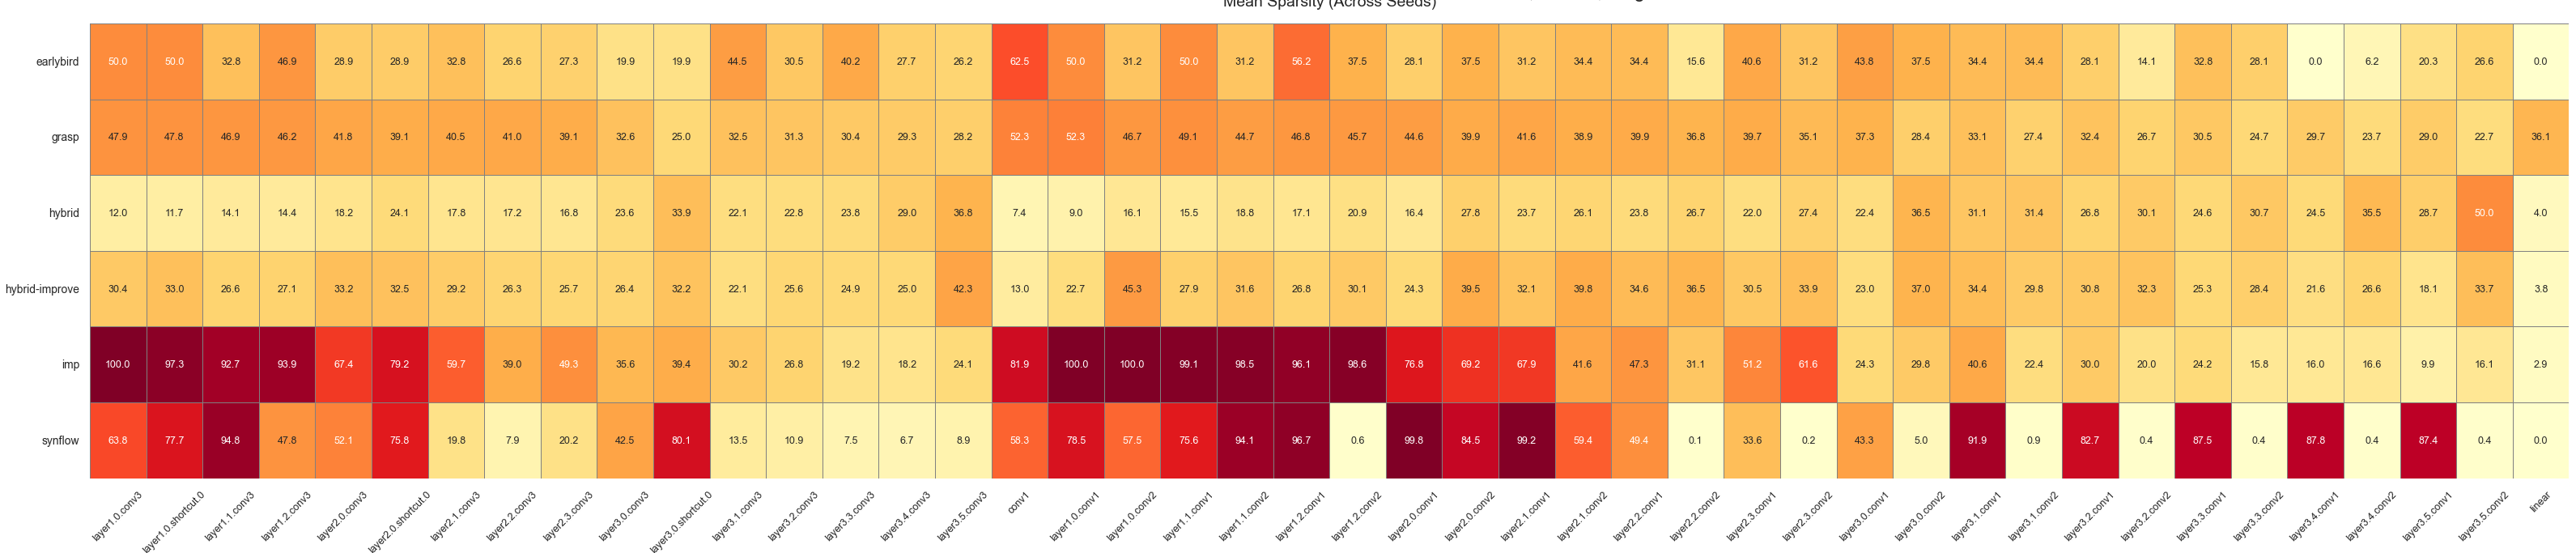
\includegraphics[width=\textwidth]{resnet50-cifar10_s0.3_heatmap.png}
                \caption{Bản đồ nhiệt phân phối độ thưa theo tầng tại $S=0{,}30$}
                \label{fig:r50_heatmap_s03}
            \end{subfigure}
            \hfill
            \begin{subfigure}{0.49\textwidth}
                \centering
                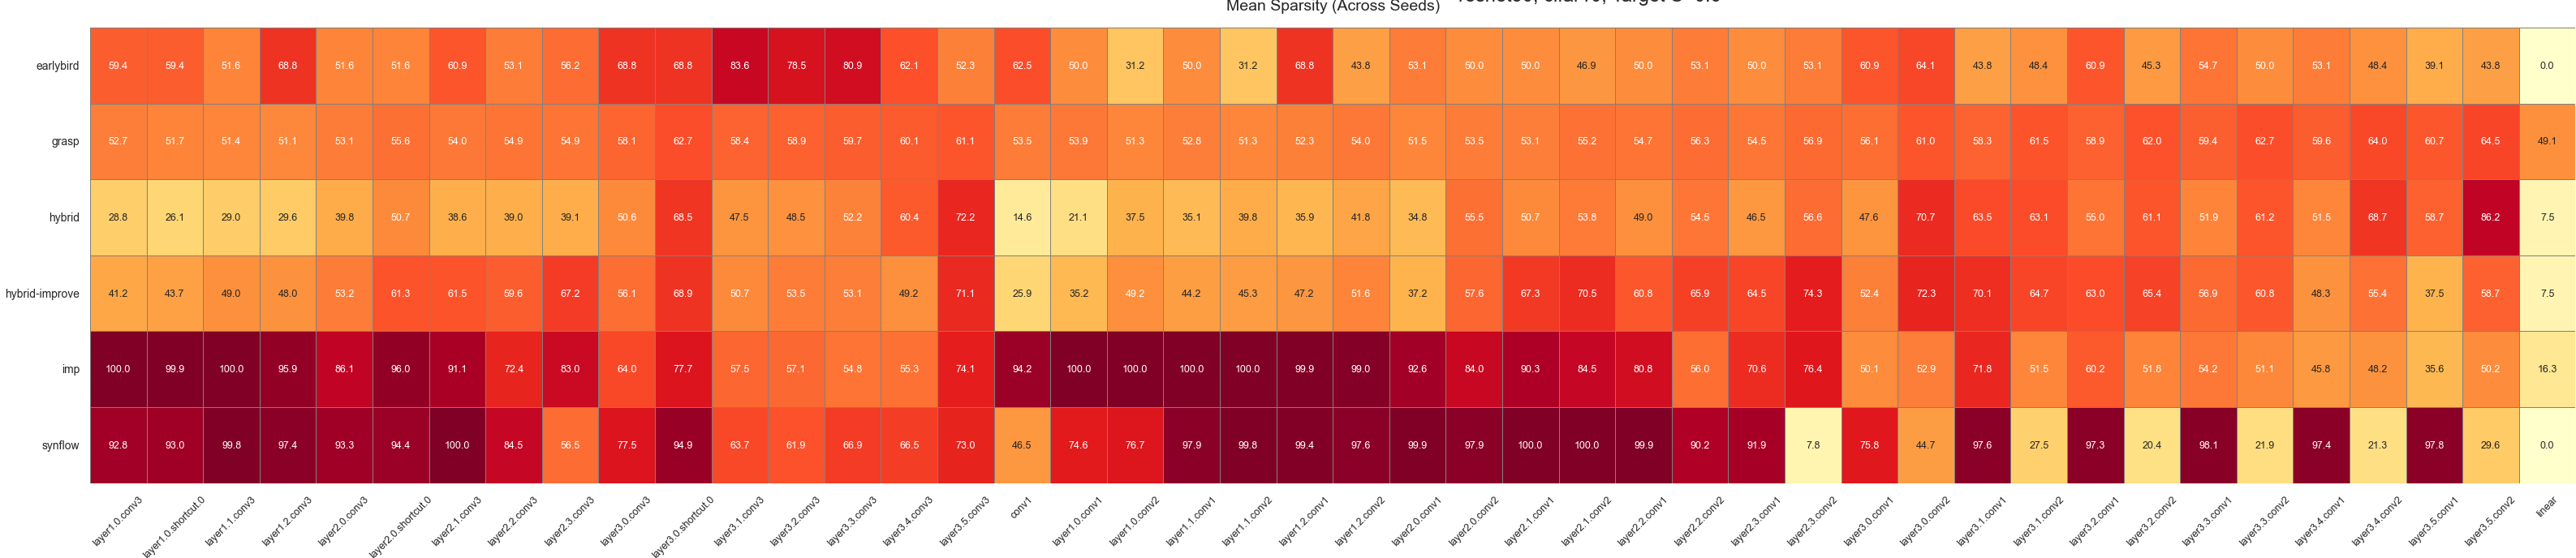
\includegraphics[width=\textwidth]{resnet50-cifar10_s0.6_heatmap.png}
                \caption{Bản đồ nhiệt phân phối độ thưa theo tầng tại $S=0{,}60$}
                \label{fig:r50_heatmap_s06}
            \end{subfigure}
            \hfill
            \begin{subfigure}{0.49\textwidth}
                \centering
                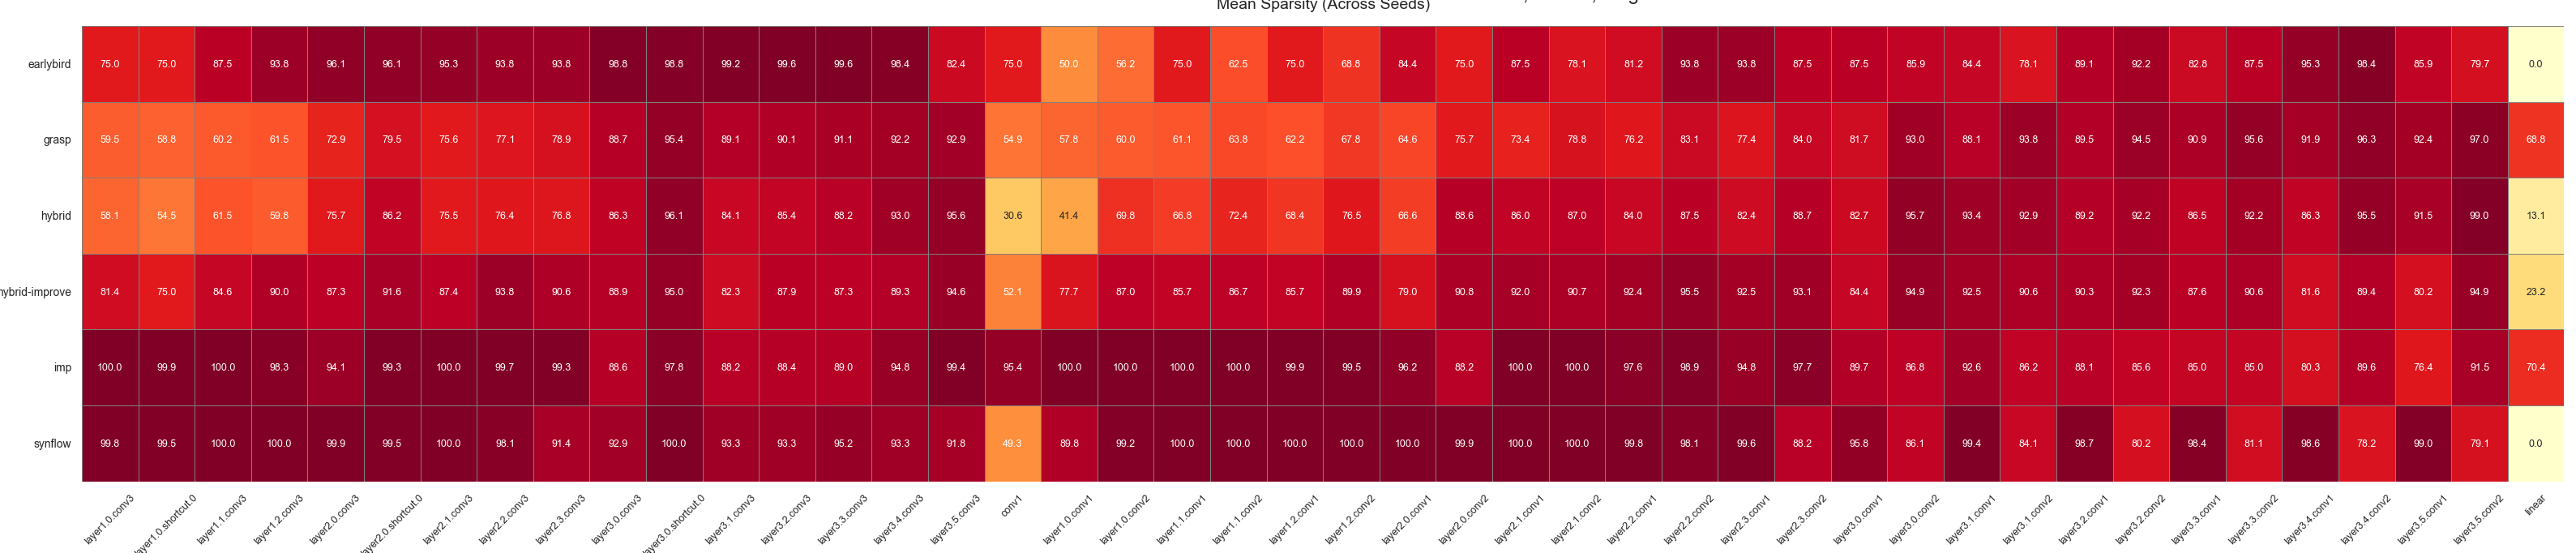
\includegraphics[width=\textwidth]{resnet50-cifar10_s0.9_heatmap.png}
                \caption{Bản đồ nhiệt phân phối độ thưa theo tầng tại $S=0{,}90$}
                \label{fig:r50_heatmap_s09}
            \end{subfigure}

            \caption{Bản đồ nhiệt phân phối độ thưa theo tầng trên CIFAR-10/ResNet-50}
            \label{fig:grouped-accuracy}
        \end{figure}
        
        Hình~\ref{fig:r50_heatmap_s03}, \ref{fig:r50_heatmap_s06} và \ref{fig:r50_heatmap_s09}
        cho thấy các mô hình định tính tương tự như ResNet-20 nhưng với sự khác biệt về cường độ.
        
        IMP trên ResNet-50 tại $S=0{,}30$ đã đẩy một số tầng shortcut đầu lên gần $100\%$ độ thưa
        ngay cả ở $S=0{,}30$ --- cực đoan hơn nhiều so với ResNet-20 ở cùng mức nén.
        Trong kiến trúc bottleneck, các tầng này chủ yếu đảm nhiệm vai trò mở rộng số chiều kênh và 
        biến đổi biểu diễn đặc trưng. Trên CIFAR-10, mức độ mở rộng này có thể dư thừa so với độ phức 
        tạp của bài toán, dẫn đến nhiều trọng số có độ lớn nhỏ và dễ bị loại bỏ.
        
        GraSP tiếp tục là phương pháp phân phối đồng đều nhất, duy trì mức độ thưa tương đương
        qua tất cả các tầng ngay cả trong kiến trúc sâu hơn, phản ánh rằng tiêu chí bảo toàn
        gradient tìm kiếm sự đồng đều về đóng góp saliency mà không bị ảnh hưởng bởi sự khác
        biệt về kích thước tầng.
        
        SynFlow tại $S=0{,}90$ cho thấy nhiều tầng shortcut đạt $\approx99\%$--$100\%$ độ thưa,
        xác nhận giả thuyết sụp đổ cấu trúc tại kết nối residual.


        \subsubsection{Mức giảm FLOPs vs chi phí huấn luyện và độ chính xác}
        Kết quả trên ResNet-50 có một số điểm khác biệt quan trọng so
        với ResNet-20.

        \begin{figure}
            \centering
            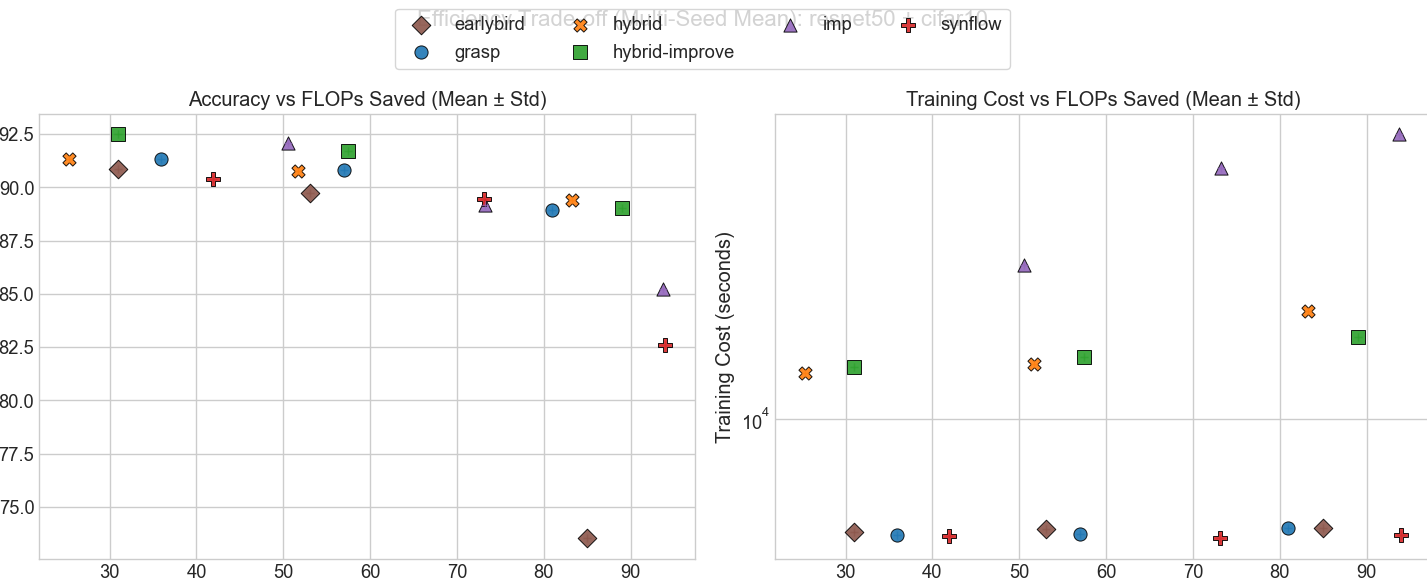
\includegraphics[width=\textwidth]{resnet50-cifar10_pareto.png}
            \caption{Biểu đồ Pareto: Cân bằng giữa độ chính xác và độ trễ trên CIFAR-10/ResNet-50}
            \label{fig:resnet50-cifar10-pareto}
        \end{figure}

        Tại $S=0{,}90$ ($\approx85\%$--$90\%$ FLOPs tiết kiệm), GraSP đạt $\approx89\%$
        độ chính xác --- xấp xỉ bằng Hybrid ($\approx89{,}7\%$) và Hybrid-Improve
        ($\approx89{,}2\%$) --- nhưng với chi phí huấn luyện thấp hơn khoảng một bậc
        độ lớn.
        Trên ResNet-20, khoảng cách accuracy giữa GraSP và các biến thể hybrid tại
        $S=0{,}90$ là $\approx2$--$3$ điểm phần trăm, đủ để biện minh cho chi phí cao
        hơn của hybrid.
        Trên ResNet-50, khoảng cách này thu hẹp xuống dưới $1$ điểm phần trăm, trong
        khi chi phí huấn luyện vẫn chênh lệch lớn.
        Điều này có nghĩa là trên ResNet-50/CIFAR-10, GraSP chiếm vị trí tốt hơn
        trên biên Pareto so với Hybrid và Hybrid-Improve khi xét đồng thời cả accuracy
        lẫn chi phí huấn luyện.

        Lý giải cho sự cải thiện tương đối này của GraSP trên ResNet-50 nằm ở đặc tính
        bảo toàn chuẩn gradient của nó: với mạng sâu hơn và nhiều tham số hơn, tiêu chí
        Hessian-gradient product của GraSP tạo ra phân phối độ thưa đồng đều hơn giữa
        các tầng, tránh được các nút thắt cổ chai mà magnitude \pruning toàn cục (IMP,
        Hybrid) dễ tạo ra khi không gian trọng số lớn hơn nhiều \cite{grasp}.
        
        % ===========================================================================
        \subsection{Độ trễ suy diễn}
        \label{sec:latency}
        % ===========================================================================
        \begin{figure}
            \centering
            \begin{subfigure}{0.49\textwidth}
                \centering
                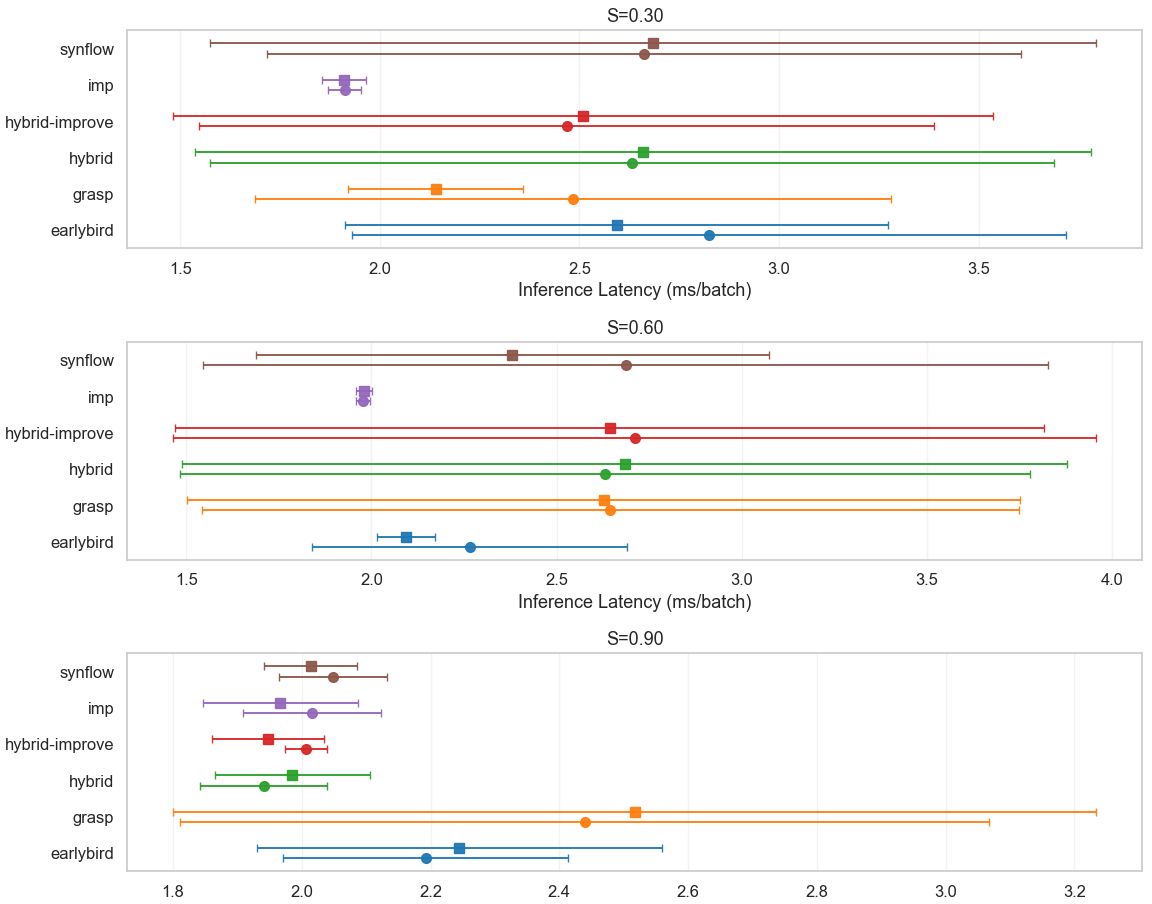
\includegraphics[width=\textwidth]{resnet20-cifar10_latency.png}
                \caption{Độ trễ suy diễn trên CIFAR-10/ResNet-20}
                \label{fig:r20c10_latency}
            \end{subfigure}
            \hfill
            \begin{subfigure}{0.49\textwidth}
                \centering
                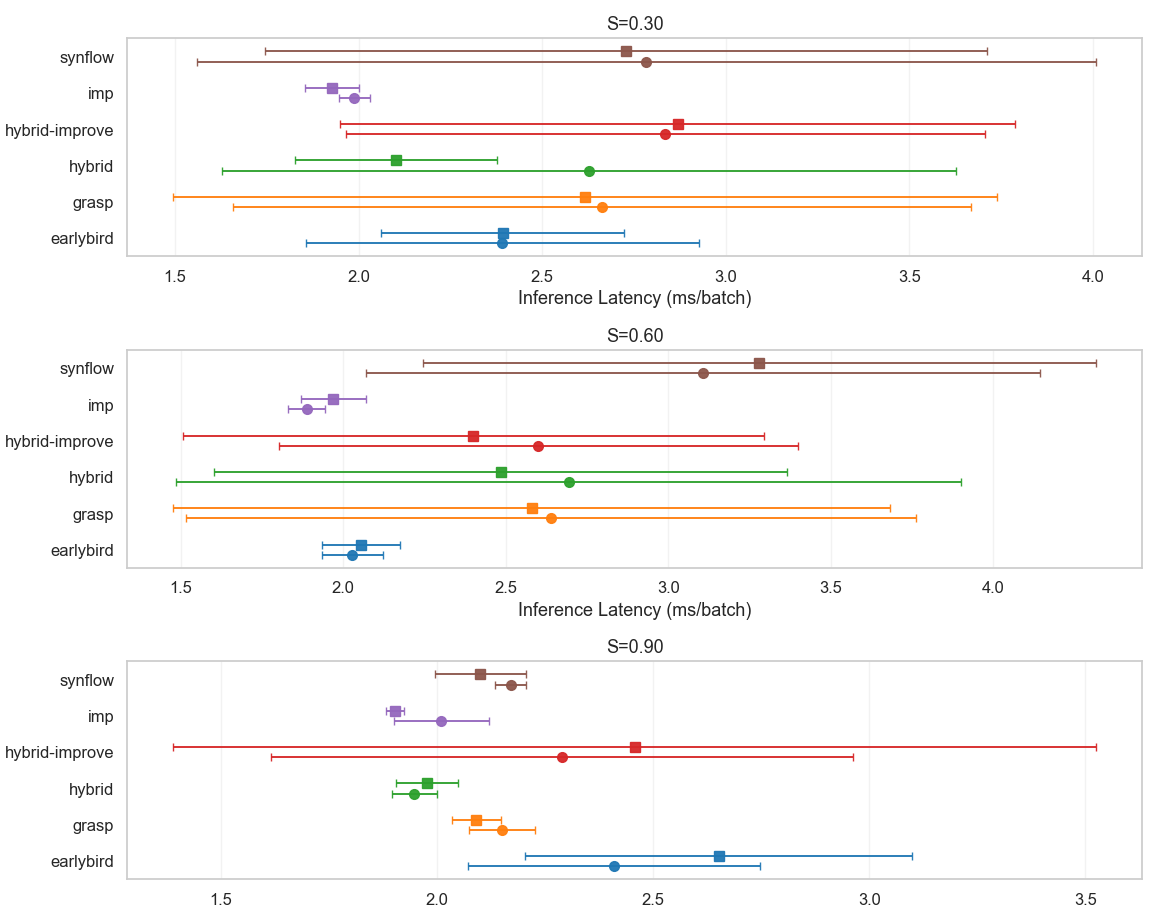
\includegraphics[width=\textwidth]{resnet20-cifar100_latency.png}
                \caption{Độ trễ suy diễn trên CIFAR-100/ResNet-20}
                \label{fig:r20c100_latency}
            \end{subfigure}
            \hfill
            \begin{subfigure}{0.49\textwidth}
                \centering
                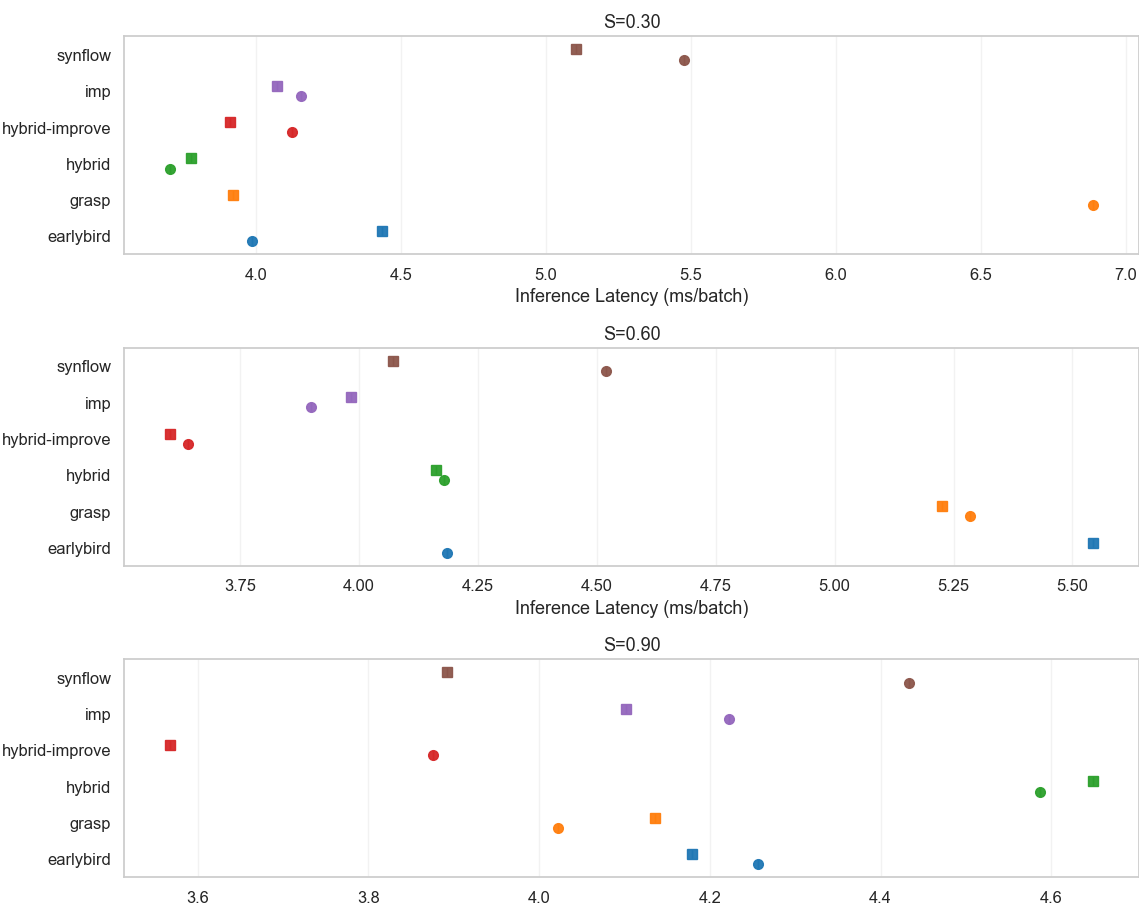
\includegraphics[width=\textwidth]{resnet50-cifar10_latency.png}
                \caption{Độ trễ suy diễn trên CIFAR-10/ResNet-50}
                \label{fig:r50_latency}
            \end{subfigure}

            \caption{So sánh độ trễ suy diễn giữa mô hình gốc và mô hình đã cắt tỉa trên các cấu hình khác nhau}
            \label{fig:grouped-accuracy}
        \end{figure}
        
        Hình~\ref{fig:r20c10_latency}, \ref{fig:r20c100_latency} và \ref{fig:r50_latency} trình
        bày so sánh độ trễ suy diễn (ms/batch) giữa mô hình gốc (hình tròn) và mô hình đã cắt tỉa
        (hình vuông) cho mỗi thuật toán và mức độ thưa.
        Quan sát nổi bật nhất là tất cả các
        phương pháp không có cấu trúc đều có thanh lỗi rất lớn về độ trễ, đặc biệt ở mức độ thưa
        thấp và vừa.
        Tại $S=0{,}30$ và $S=0{,}60$ trên ResNet-20, thanh lỗi của nhiều thuật toán (SynFlow,
        Hybrid, Hybrid-Improve, GraSP, Early-Bird) trải rộng hơn $2$ ms --- gần bằng toàn bộ dải
        giá trị đo được.
        Điều này có nghĩa là sự khác biệt quan sát được giữa mô hình gốc và mô hình đã cắt tỉa
        nằm hoàn toàn trong vùng nhiễu đo lường.
        Đến $S=0{,}90$, các thanh lỗi thu hẹp đáng kể (khoảng $\pm0{,}1$--$0{,}3$ ms), nhưng
        lúc này sự khác biệt giữa dense và pruned cũng biến mất --- mọi thuật toán tập trung trong
        khoảng $1{,}8$--$2{,}6$ ms/batch với ResNet-20.
% \chapter{Kết quả}
\label{ch:results}

\section{CIFAR-10 / ResNet-20}

\subsection{Độ chính xác theo mức độ thưa}
\begin{figure}[h]
	\centering
	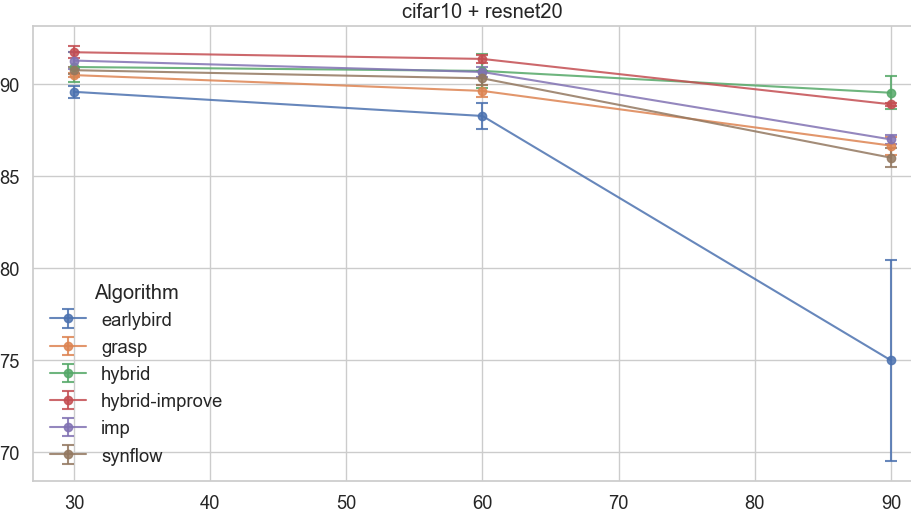
\includegraphics[width=\textwidth]{resnet20-cifar10_acc+sparsity.png}
	\caption{Độ chính xác theo mức độ thưa trên CIFAR-10/ResNet-20}
	\label{fig:resnet20-cifar10-acc-sparsity}
\end{figure}
Có thể thấy có 2 nhóm hành vi:
 
\paragraph{Nhóm suy giảm từ từ:}

GraSP, SynFlow, Hybrid, Hybrid-Improve và IMP đều duy trì độ chính xác trong khoảng
$85\%$--$91{,}5\%$ qua tất cả các mức độ thưa.
Tại $S=0{,}30$, Hybrid-Improve dẫn đầu ($\approx91{,}2\%$), xấp xỉ bằng mô hình gốc,
trong khi IMP, Hybrid, GraSP và SynFlow dao động trong khoảng $90{,}0\%$--$91{,}0\%$.
Đáng chú ý, sụt giảm của Hybrid-Improve tại $S=0{,}30$ xấp xỉ bằng không, tức là mô
hình sau cắt tỉa nhẹ gần như tương đương mô hình gốc.
Tại $S=0{,}90$, Hybrid và Hybrid-Improve tiếp tục dẫn đầu ($\approx89\%$--$89{,}5\%$),
tiếp theo là GraSP và IMP ($\approx87\%$), trong khi SynFlow sụt giảm đến $\approx85\%$.

\paragraph{Nhóm sụp đổ hiệu năng.}
Early-Bird có hành vi hoàn toàn khác biệt.
Ngay tại $S=0{,}30$, độ chính xác của nó ($\approx89{,}5\%$) đã thấp hơn tất cả các
thuật toán còn lại, và tiếp tục sụt giảm mạnh: $\approx88{,}3\%$ tại $S=0{,}60$, và
$\approx75\%$ tại $S=0{,}90$ --- mất hơn $16$ điểm phần trăm so với mô hình gốc.
Quan trọng hơn, thanh sai số của Early-Bird tại $S=0{,}90$ là rộng nhất trong tất cả các
thuật toán (độ lệch chuẩn $\approx5\%$--$6\%$), cho thấy hành vi của nó ở độ thưa cao
không chỉ kém mà còn không ổn định giữa các hạt giống khác nhau.
Nguyên nhân nằm ở bản chất của Early-Bird: điểm quan trọng kênh được tính từ hệ số
co giãn Batch Normalisation ($\gamma$) tại các epoch rất sớm (thường $6\%$--$20\%$ tổng
số epoch), khi mô hình chưa hội tụ. Tại $S=0{,}90$, các điểm số này quá nhiễu và nhạy
cảm với khởi tạo khác nhau, dẫn đến việc lựa chọn kênh quan trọng sai và không nhất quán.

\subsection{Sụt giảm độ chính xác}

\begin{figure}[h]
	\centering
	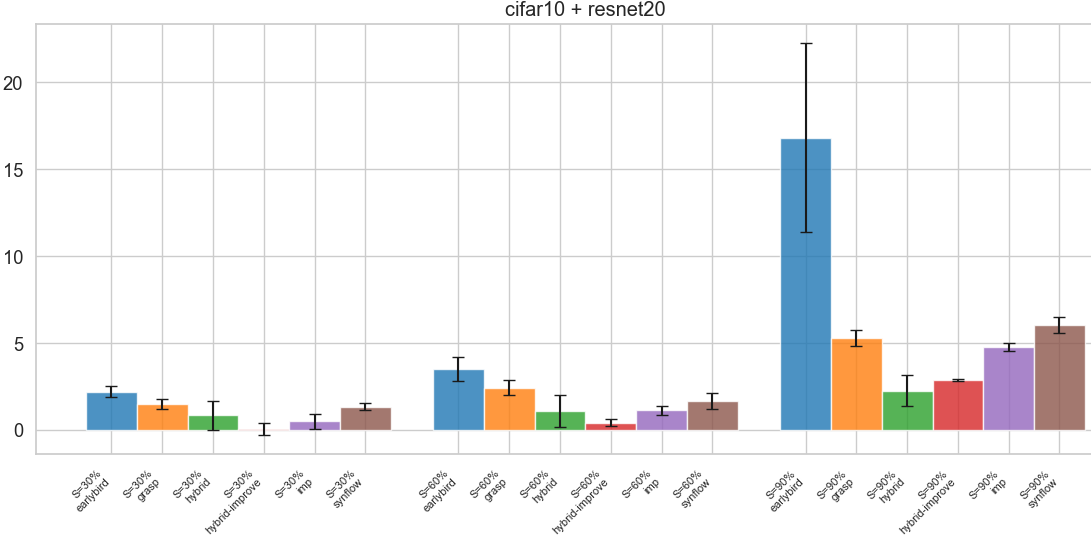
\includegraphics[width=\textwidth]{resnet20-cifar10_accdrop.png}
	\caption{Mức giảm độ chính xác so với mô hình dày đặc trên CIFAR-10/ResNet-20}
	\label{fig:resnet20-cifar10-accdrop}
\end{figure}
\label{subsec:r20c10_drop}
 
Hình~\ref{fig:resnet20-cifar10-accdrop} biểu diễn sụt giảm độ chính xác trung bình và độ lệch chuẩn
qua các hạt giống cho mỗi thuật toán tại từng mức độ thưa.
 
Tại $S=0{,}30$, sụt giảm của tất cả các thuật toán ngoài Early-Bird đều nhỏ và tập trung:
Hybrid-Improve $\approx0{,}0\%$, IMP $\approx0{,}5\%$, Hybrid $\approx0{,}9\%$,
SynFlow $\approx1{,}4\%$ và GraSP $\approx1{,}5\%$.
Thanh lỗi nhỏ ở mức này xác nhận rằng $S=0{,}30$ nằm trong vùng nén an toàn cho
ResNet-20 với tất cả các phương pháp không có cấu trúc.
 
Tại $S=0{,}60$, thứ hạng được giữ nguyên: Hybrid-Improve vẫn dẫn đầu ($\approx0{,}5\%$),
tiếp theo là Hybrid ($\approx1{,}1\%$), IMP ($\approx1{,}3\%$), SynFlow ($\approx1{,}7\%$)
và GraSP ($\approx2{,}4\%$).
 
Điều quan trọng nhất nằm ở $S=0{,}90$.
Early-Bird đạt sụt giảm trung bình $\approx17\%$ với độ lệch chuẩn $\approx6\%$ --- một
mức biến động cực kỳ cao, có nghĩa là trong điều kiện tệ nhất, mô hình có thể mất hơn
$23\%$ độ chính xác.
Trong số các phương pháp còn lại, Hybrid dẫn đầu với chỉ $\approx2{,}2\%$ sụt giảm,
tiếp theo là Hybrid-Improve ($\approx3{,}0\%$), IMP ($\approx5{,}0\%$), GraSP
($\approx5{,}5\%$) và SynFlow ($\approx6{,}2\%$).
 
Đáng chú ý, Hybrid ở $S=0{,}90$ vượt qua Hybrid-Improve theo
giá trị trung bình. Tuy nhiên, biên độ độ chính xác của Hybrid lớn hơn đáng kể so với 
Hybrid-Improve, do đó vẫn có thể nói rằng Hybrid-Improve có hiệu suất ổn định hơn ở mức độ thưa cực cao.
\subsection{Mức giảm FLOPs vs chi phí huấn luyện và độ chính xác}
\label{subsec:r20c10_efficiency}
\noindent
\begin{figure}[h]
	\centering
	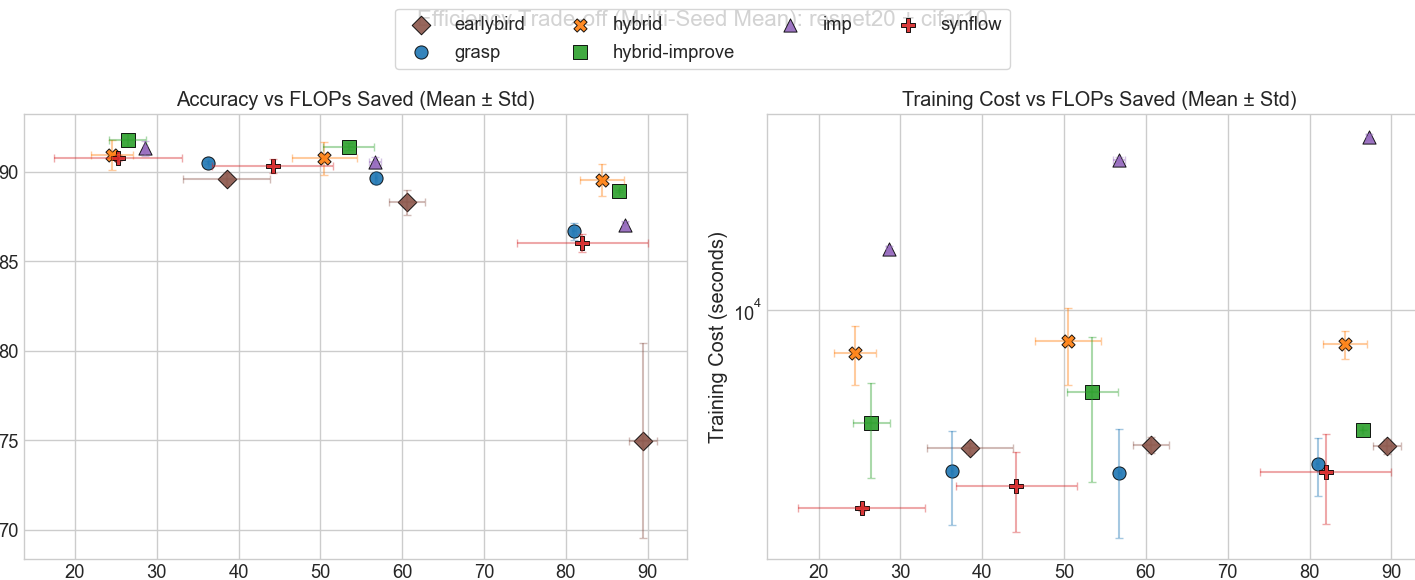
\includegraphics[width=\textwidth]{resnet20-cifar10_pareto.png}
	\caption{Biểu đồ Pareto: Cân bằng giữa độ chính xác và độ trễ trên CIFAR-10/ResNet-20}
	\label{fig:resnet20-cifar10-pareto}
\end{figure}

Hình~\ref{fig:resnet20-cifar10-pareto} trình bày hai biểu đồ phân tán: (trái) độ chính xác so
với mức giảm FLOPs tiết kiệm, và (phải) chi phí huấn luyện so với mức giảm FLOPs.
Cả hai đều hiển thị giá trị trung bình và thanh lỗi qua nhiều hạt giống.
 
Cần lưu ý rằng mức giảm FLOPs được ước lượng theo mật độ mặt nạ và là các giá trị lý thuyết, không phải phép đo phần
cứng thực tế.
 
Tại tỉ lệ giảm FLOPs $\approx20\%$--$50\%$, GraSP, Hybrid và Hybrid-Improve
tập trung gần phía trên của trục độ chính xác ($\approx90\%$--$91\%$), cho thấy chúng
là các phương pháp hiệu quả nhất khi nén nhẹ.
Ở tỉ lệ giảm FLOPs $>80\%$, Hybrid và Hybrid-Improve
nằm trên biên Pareto với $\approx89\%$--$89{,}5\%$, tiếp theo là GraSP và IMP ở
$\approx87\%$.
 
Về chi phí huấn luyện, IMP là đắt nhất ở mọi mức độ thưa ($10^4$--$10^5$ giây), do có
nhiều vòng prune-retrain-rewind. Hybrid và Hybrid-Improve ở mức trung gian, trong khi
GraSP và SynFlow rẻ nhất vì chỉ cần 1 lần cắt tỉa và một lần huấn luyện.
Tuy nhiên, kết quả cho thấy IMP có biến động chi phí thấp, trong
khi Hybrid và Hybrid-Improve có biến động vừa phải tùy thuộc vào khi nào điều kiện dừng
sớm (early stopping) được kích hoạt. % original hybrid paper suggests this

\subsection{Phân phối độ thưa theo tầng và tính ổn định}
\label{subsec:r20c10_layerwise}

\begin{figure}[h]
    \centering
    \begin{subfigure}{0.49\textwidth}
        \centering
        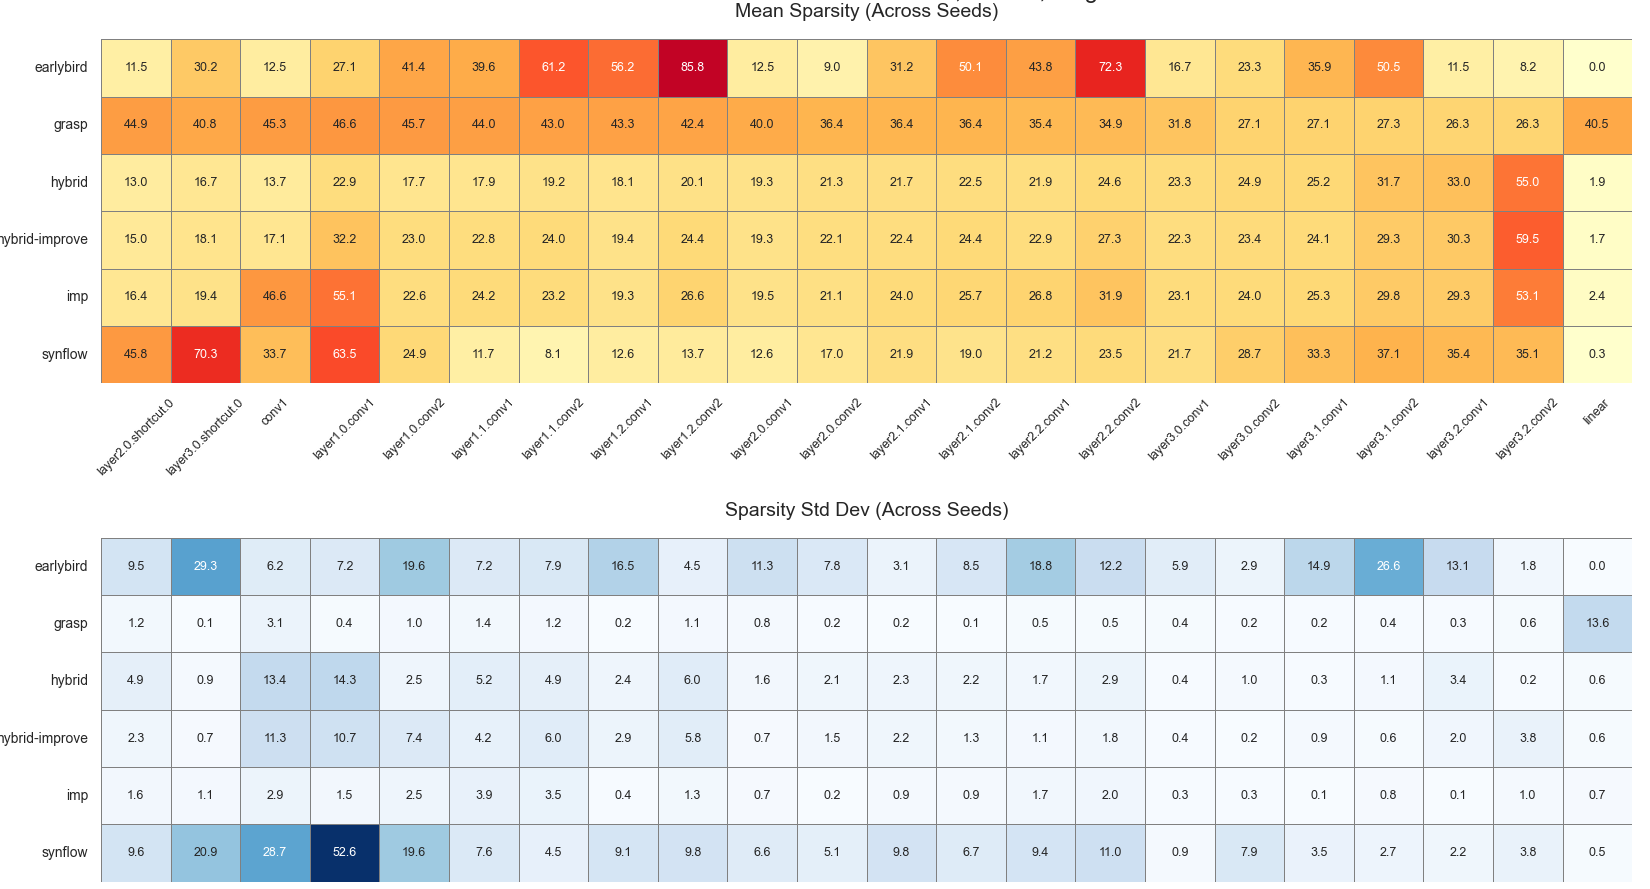
\includegraphics[width=\textwidth]{resnet20-cifar10_s0.3_heatmap.png}
        \caption{Bản đồ nhiệt phân phối độ thưa theo tầng tại $S=0{,}30$}
        \label{fig:r20c10_heatmap_s03}
    \end{subfigure}
    \hfill
    \begin{subfigure}{0.49\textwidth}
        \centering
        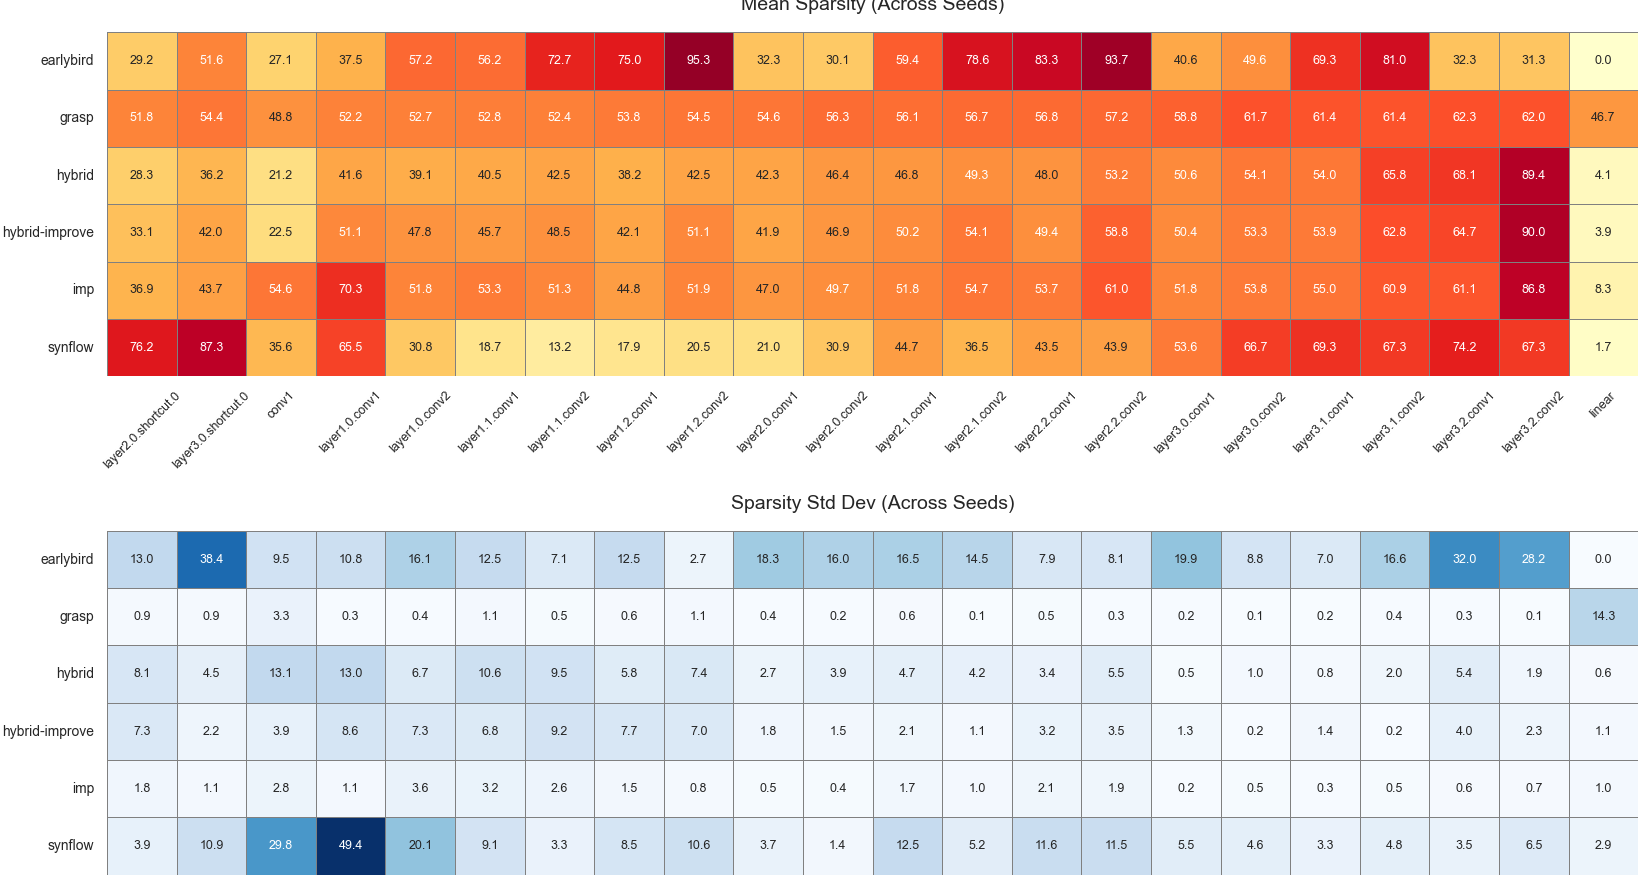
\includegraphics[width=\textwidth]{resnet20-cifar10_s0.6_heatmap.png}
        \caption{Bản đồ nhiệt phân phối độ thưa theo tầng tại $S=0{,}60$}
        \label{fig:r20c10_heatmap_s06}
    \end{subfigure}
    \hfill
    \begin{subfigure}{0.49\textwidth}
        \centering
        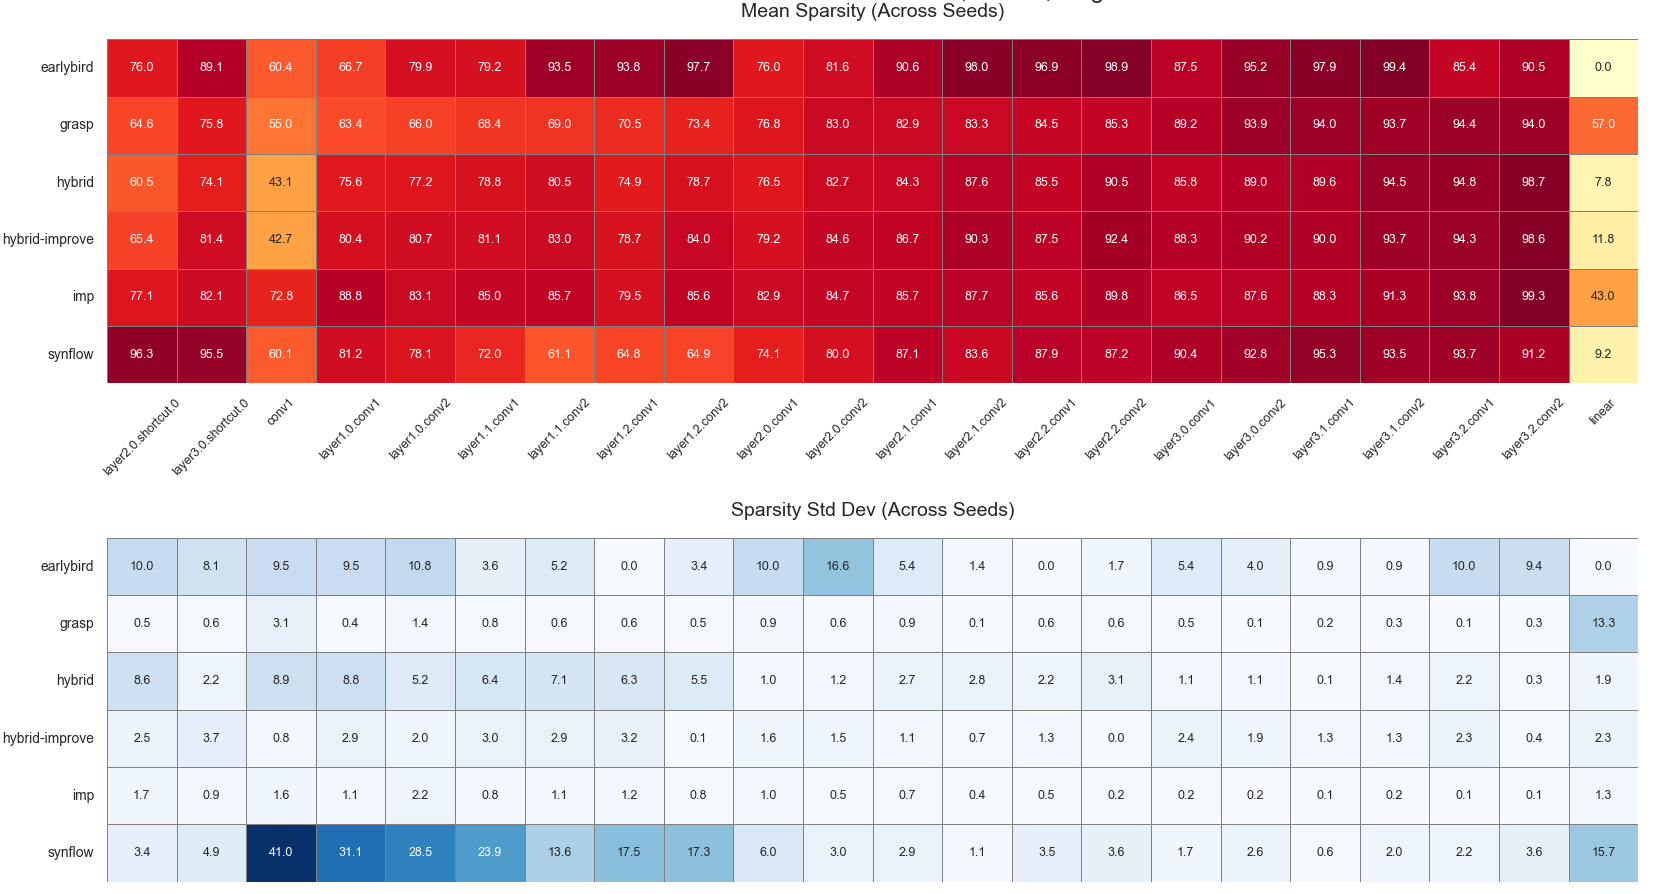
\includegraphics[width=\textwidth]{resnet20-cifar10_s0.9_heatmap.png}
        \caption{Bản đồ nhiệt phân phối độ thưa theo tầng tại $S=0{,}90$}
        \label{fig:r20c10_heatmap_s09}
    \end{subfigure}

    \caption{Bản đồ nhiệt phân phối độ thưa theo tầng trên CIFAR-10/ResNet-20}
    \label{fig:grouped-accuracy}
\end{figure}
 
Hình~\ref{fig:r20c10_heatmap_s03}, \ref{fig:r20c10_heatmap_s06} và
\ref{fig:r20c10_heatmap_s09} hiển thị cả bản đồ nhiệt trung bình và
độ lệch chuẩn của phân phối độ thưa theo tầng qua các cài đặt.
 
GraSP cho thấy phân phối độ thưa đồng đều nhất qua tất cả các tầng ở cả ba mức độ thưa,
với độ lệch chuẩn rất thấp trên hầu hết các tầng.
Tính đồng đều trong phân phối của GraSP là hệ quả trực tiếp từ tiêu chí bảo toàn chuẩn gradient: vì chuẩn gradient
phụ thuộc vào luồng thông tin qua toàn bộ mạng, bất kỳ tầng nào bị cắt tỉa quá mạnh đều tạo ra
nút thắt cổ chai làm giảm gradient toàn cục, khiến các trọng số tại tầng đó nhận điểm saliency
cao và được bảo vệ, điều này tự nhiên khuyến khích cắt tỉa đồng đều trên tất cả các tầng.
 
IMP cũng có độ lệch chuẩn rất thấp qua các tầng, điều này có thể giải thích bởi tính xác định
cao của tiêu chí magnitude sau huấn luyện đầy đủ — các trọng số hội tụ về vùng tương tự qua
các hạt giống, dẫn đến ngưỡng cắt tỉa toàn cục nhất quán. % Morcos et al. (2019) "One ticket to win them all" cho thấy winning ticket có thể transfer qua datasets
Tuy nhiên, IMP tập trung độ thưa cao hơn vào các tầng đầu (ví dụ
\texttt{layer1.0.conv1}: $55{,}1\%$ tại $S=0{,}30$), Điều này có thể giải thích do
các tầng đầu của ResNet-20 trên CIFAR-10 thường học các đặc trưng mức thấp như cạnh
và kết cấu đơn giản, do đó có thể chứa nhiều trọng số dư thừa hoặc có độ lớn nhỏ. Vì
vậy, các tầng này thường bị cắt tỉa mạnh hơn.
Cả hai biến thể hybrid đều thể hiện xu hướng bảo vệ tầng đầu: tầng \texttt{conv1}
chỉ đạt $\approx13\%$--$17\%$ độ thưa tại $S=0{,}30$, trong khi các tầng sâu hơn nhận
được cắt tỉa nhiều hơn (ví dụ \texttt{layer3.2.conv2}: $55\%$--$59{,}5\%$).
Độ lệch chuẩn ở mức trung bình --- 
phản ánh sự kết hợp của hai giai đoạn cắt tỉa (one-shot và lặp). 

SynFlow là thuật toán kém ổn định nhất trong số các phương pháp được đánh giá.
Tại $S=0{,}30$, độ lệch chuẩn đạt tới $52{,}6\%$ tại \texttt{layer1.0.conv1} và $28{,}7\%$
tại \texttt{conv1}. Điều này có nghĩa là quyết định phân bổ độ thưa cho các tầng quan
trọng này thay đổi rất lớn giữa các hạt giống.
Nguyên nhân nằm ở tính nhạy cảm của điểm SynFlow đối với giá trị khởi tạo ngẫu nhiên:
vì điểm path-norm được tính tại thời điểm khởi tạo mà không dùng dữ liệu thực, các trọng % 
số được khởi tạo khác nhau sẽ tạo ra phân phối điểm rất khác nhau.
Sự không ổn định trong phân phối độ thưa theo tầng trực tiếp giải thích sự biến động cao
trong độ chính xác cuối cùng của SynFlow qua các hạt giống.
 
Bản đồ độ lệch chuẩn của Early-Bird cho thấy biến động lớn ở nhiều tầng, đặc biệt ở các
kết nối shortcut và các tầng conv đầu (ví dụ \texttt{layer3.0.shortcut.0}: $\sigma=26{,}6\%$ % wrong data
tại $S=0{,}30$).
Điều này xác nhận rằng các điểm quan trọng kênh dựa trên hệ số $\gamma$ BN ở giai đoạn
huấn luyện sớm không ổn định và phụ thuộc nhiều vào hạt giống khởi tạo, dẫn đến các quyết
định cắt tỉa cấu trúc khác nhau và do đó độ chính xác khác nhau đáng kể giữa các lần chạy


\section{CIFAR-100/ResNet-20}

CIFAR-100 là bộ dữ liệu khó hơn đáng kể so với CIFAR-10: $100$ lớp thay vì $10$ lớp,
với $600$ ảnh mỗi lớp thay vì $6000$, đòi hỏi mô hình phải học các đặc trưng phân biệt
tinh tế hơn với ít dữ liệu huấn luyện hơn mỗi lớp.
Khi áp dụng cùng các thuật toán cắt tỉa trên cấu hình ResNet-20/CIFAR-100, tác động của cắt tỉa sẽ nghiêm trọng hơn, đặc biệt ở mức độ thưa cao, vì mạng cần
duy trì khả năng phân biệt giữa nhiều lớp hơn với ít tham số hơn.
 
\subsection{Độ chính xác và sụt giảm theo mức độ thưa}
\label{subsec:r20c100_acc}

\begin{figure}[h]
    \centering

    \begin{subfigure}{0.49\textwidth}
        \centering
        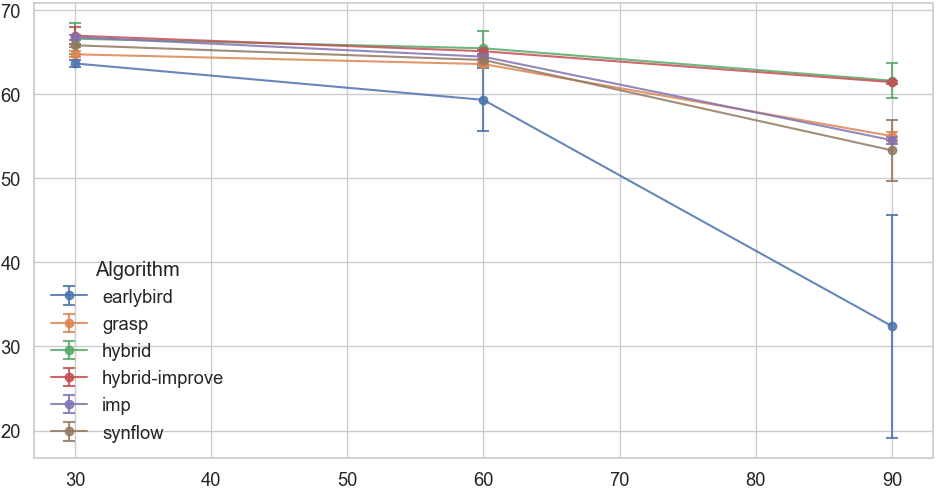
\includegraphics[width=\textwidth]{resnet20-cifar100_acc+sparsity.png}
        \caption{Độ chính xác theo mức độ thưa trên CIFAR-100/ResNet-20}
        \label{fig:resnet20-cifar100-acc-sparsity}
    \end{subfigure}
    \hfill
    \begin{subfigure}{0.49\textwidth}
        \centering
        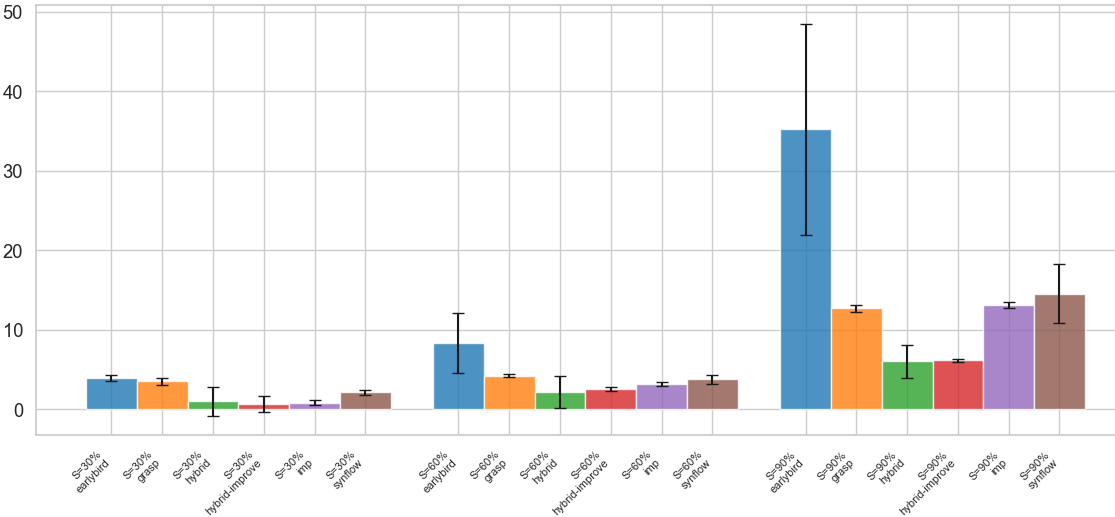
\includegraphics[width=\textwidth]{resnet20-cifar100_accdrop.png}
        \caption{Mức giảm độ chính xác so với mô hình dày đặc trên CIFAR-100/ResNet-20}
        \label{fig:resnet20-cifar100-accdrop}
    \end{subfigure}

    \caption{Độ chính xác theo mức độ thưa trên CIFAR-100/ResNet-20}
    \label{fig:grouped-accuracy}
\end{figure}
 
Hình~\ref{fig:resnet20-cifar100-acc-sparsity} và \ref{fig:resnet20-cifar100-accdrop} cho thấy xu hướng tương tự như
CIFAR-10 nhưng với mức sụt giảm lớn hơn đáng kể.
 
Tại $S=0{,}30$, Hybrid và Hybrid-Improve gần như không sụt giảm ($\approx1{,}0\%$ và
$\approx0{,}7\%$ tương ứng), trong khi IMP sụt giảm $\approx0{,}7\%$, SynFlow $\approx2{,}5\%$,
GraSP và Early-Bird cùng $\approx3{,}8\%$.
Thanh lỗi nhỏ cho hầu hết các thuật toán ở mức này cho thấy $S=0{,}30$ vẫn trong vùng
nén an toàn trên CIFAR-100 với các phương pháp không có cấu trúc.
 
Tại $S=0{,}60$, khoảng cách giữa các thuật toán bắt đầu mở rộng rõ rệt.
Early-Bird sụt giảm $\approx8{,}5\%$ với thanh lỗi lớn, cho thấy độ không ổn định đặc
trưng của nó.
Hybrid ($\approx2{,}2\%$) và Hybrid-Improve ($\approx2{,}5\%$) vẫn duy trì hiệu suất tốt.
GraSP ($\approx4\%$), IMP ($\approx3\%$) và SynFlow ($\approx4\%$) ở mức trung gian.
 
Tại $S=0{,}90$, sự phân hóa trở nên cực kỳ rõ ràng:
\begin{itemize}
    \item \textbf{Early-Bird:} sụt giảm trung bình $\approx35\%$ với độ lệch chuẩn lên
    đến $\approx13\%$. Trong điều kiện tệ nhất (mean + 1 std), độ chính xác có thể rơi
    xuống dưới $20\%$ --- gần như không thể sử dụng được. Đây là hành vi sụp đổ nghiêm
    trọng nhất trong toàn bộ thực nghiệm.
    \item \textbf{GraSP và IMP:} cùng sụt giảm $\approx13\%$ --- lớn hơn gấp đôi so với
    CIFAR-10 ở cùng mức độ thưa.
    \item \textbf{SynFlow:} sụt giảm $\approx14{,}5\%$ --- lớn hơn đáng kể so với CIFAR-10
    ($\approx6{,}2\%$).
    \item \textbf{Hybrid và Hybrid-Improve:} cùng sụt giảm $\approx6\%$, dẫn đầu so với các
    thuật toán khác với biên độ tương đối nhỏ.
\end{itemize}
 
Việc mức sụt giảm lớn hơn đối với GraSP, IMP và SynFlow trên CIFAR-100 là có thể dự đoán được.
Trên CIFAR-100, mỗi tham số mang nhiều thông tin phân loại hơn
do phải phân biệt $10\times$ nhiều lớp hơn với $10\times$ ít dữ liệu hơn mỗi lớp hơn so với CIFAR-10.
Cắt tỉa $90\%$ tham số do đó loại bỏ nhiều thông tin không thể phục hồi hơn, và khả năng
phục hồi thông qua tinh chỉnh bị hạn chế hơn vì tập dữ liệu nhỏ hơn theo lớp.
Các biến thể hybrid vẫn vượt trội nhờ chiến lược phân giai đoạn: cắt tỉa từ từ và tinh
chỉnh với kiên nhẫn sau mỗi bước đặc biệt quan trọng khi tập dữ liệu nhỏ hơn theo lớp,
vì mô hình cần nhiều epoch hơn để hội tụ lại sau mỗi bước cắt tỉa.
 
\subsection{Phân phối độ thưa theo tầng và tính ổn định}
\label{subsec:r20c100_layerwise}

\begin{figure}[h]
	\centering
	\begin{subfigure}{0.49\textwidth}
		\centering
		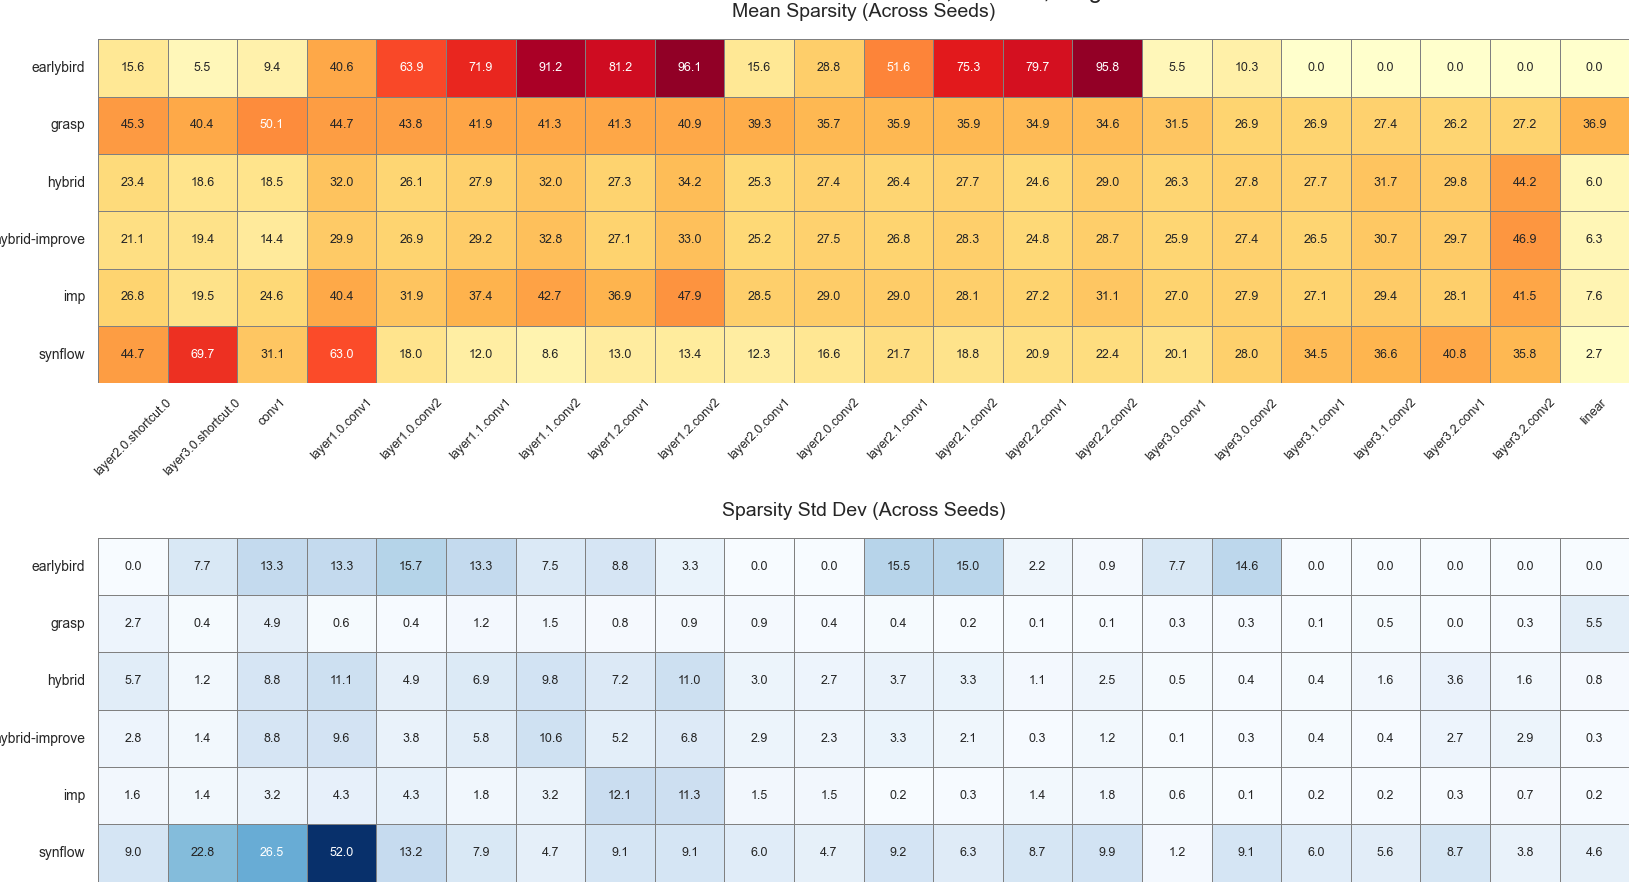
\includegraphics[width=\textwidth]{resnet20-cifar100_s0.3_heatmap.png}
		\caption{Bản đồ nhiệt phân phối độ thưa theo tầng tại $S=0{,}30$}
		\label{fig:r20c100_heatmap_s03}
	\end{subfigure}
	\hfill
	\begin{subfigure}{0.49\textwidth}
		\centering
		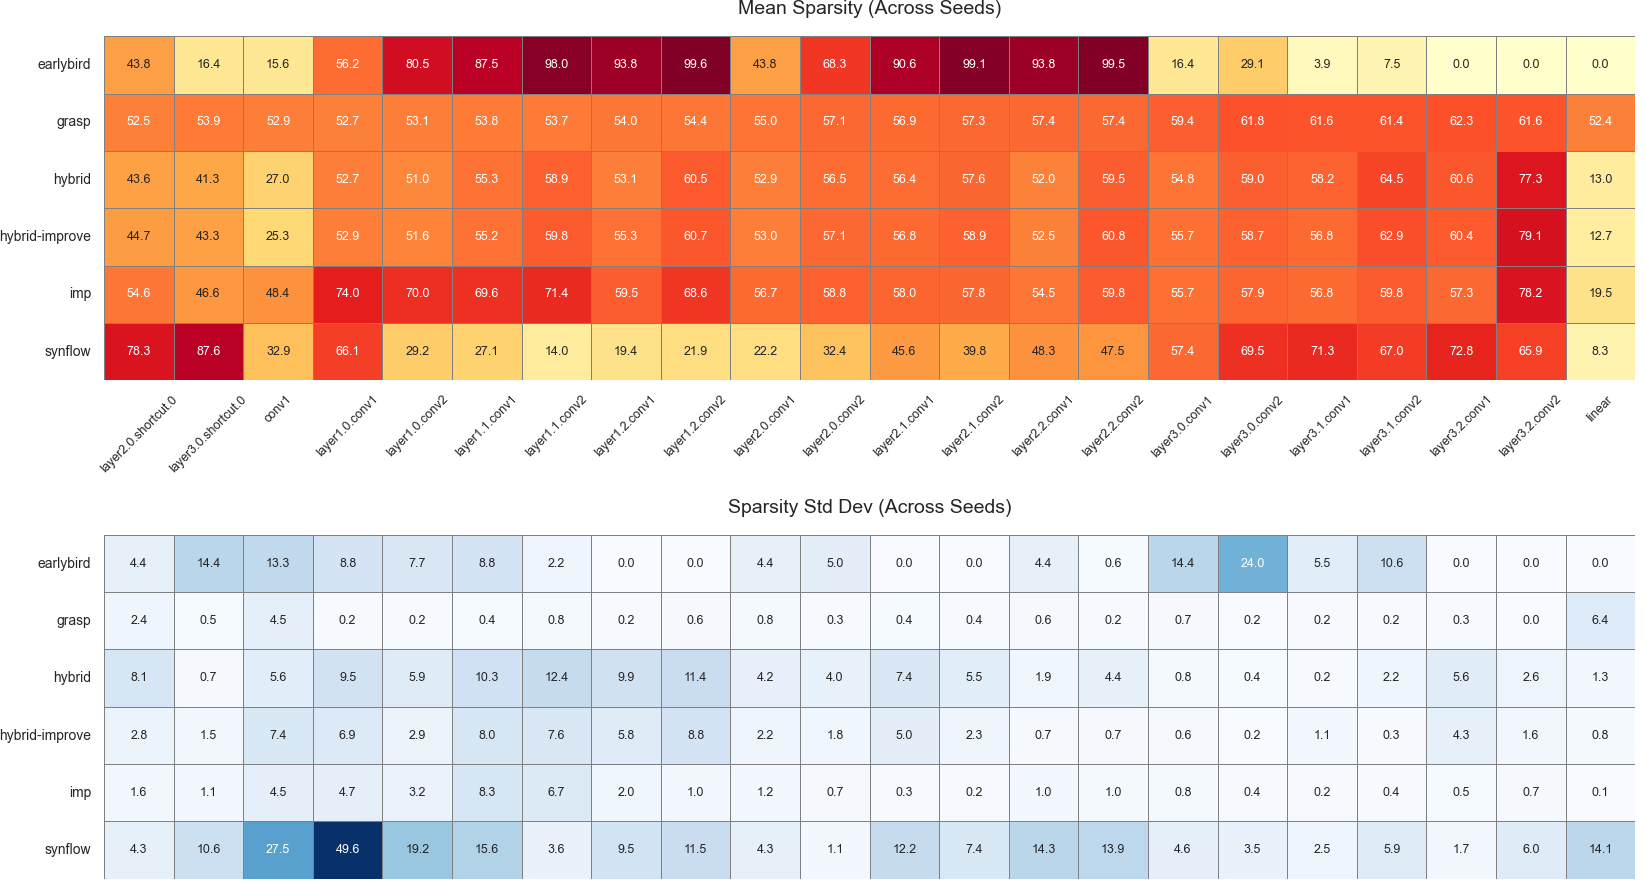
\includegraphics[width=\textwidth]{resnet20-cifar100_s0.6_heatmap.png}
		\caption{Bản đồ nhiệt phân phối độ thưa theo tầng tại $S=0{,}60$}
		\label{fig:r20c100_heatmap_s06}
	\end{subfigure}
	\hfill
	\begin{subfigure}{0.49\textwidth}
		\centering
		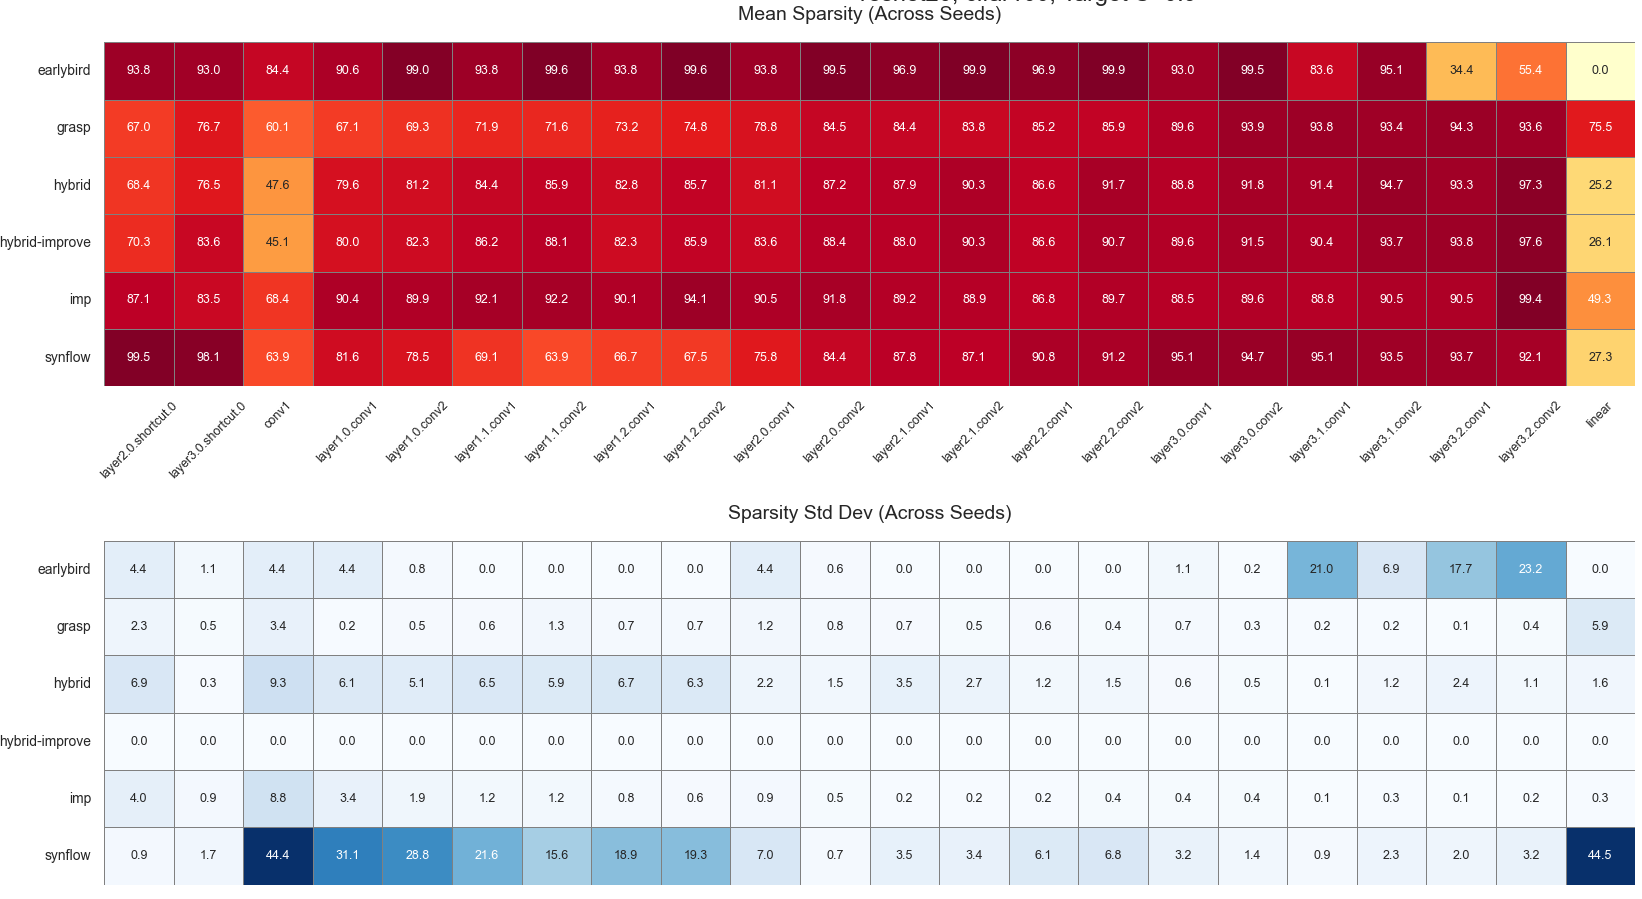
\includegraphics[width=\textwidth]{resnet20-cifar100_s0.9_heatmap.png}
		\caption{Bản đồ nhiệt phân phối độ thưa theo tầng tại $S=0{,}90$}
		\label{fig:r20c100_heatmap_s09}
	\end{subfigure}

	\caption{Bản đồ nhiệt phân phối độ thưa theo tầng trên CIFAR-100/ResNet-20}
	\label{fig:grouped-accuracy}
\end{figure}
 
Hình~\ref{fig:r20c100_heatmap_s03}, \ref{fig:r20c100_heatmap_s06} và
\ref{fig:r20c100_heatmap_s09} cho thấy các xu hướng phân phối tương tự như CIFAR-10 nhưng
với một số điểm khác biệt đáng chú ý.

Early-Bird trên CIFAR-100 tại $S=0{,}30$ đã có nhiều tầng đạt $>90\%$ độ thưa kênh
(ví dụ \texttt{layer1.2.conv2}: $96{,}1\%$; \texttt{layer3.0.shortcut.0}: $95{,}8\%$),
sớm và cực đoan hơn nhiều so với CIFAR-10.
Điều này cho thấy điểm $\gamma$ BN trên CIFAR-100 tạo ra phân phối thưa kênh nghiêm trọng
hơn ngay cả ở mức nén nhẹ --- một phần vì mô hình trên CIFAR-100 học được ít kênh ``dư
thừa'' hơn, khiến các điểm $\gamma$ phân biệt rõ hơn và dẫn đến cắt tỉa hung hăng hơn.
 
SynFlow trên CIFAR-100 duy trì mô hình độ lệch chuẩn cao ở các tầng đầu
(\texttt{conv1}: $\sigma=26{,}5\%$; \texttt{layer1.0.conv1}: $\sigma=52{,}0\%$ tại $S=0{,}30$),
xác nhận rằng sự không ổn định của SynFlow là đặc trưng của phương pháp chứ không phải
của bộ dữ liệu cụ thể.
 
\subsection{Mức giảm FLOPs vs chi phí huấn luyện và độ chính xác}
\label{subsec:r20c100_efficiency}

\begin{figure}[h]
	\centering
	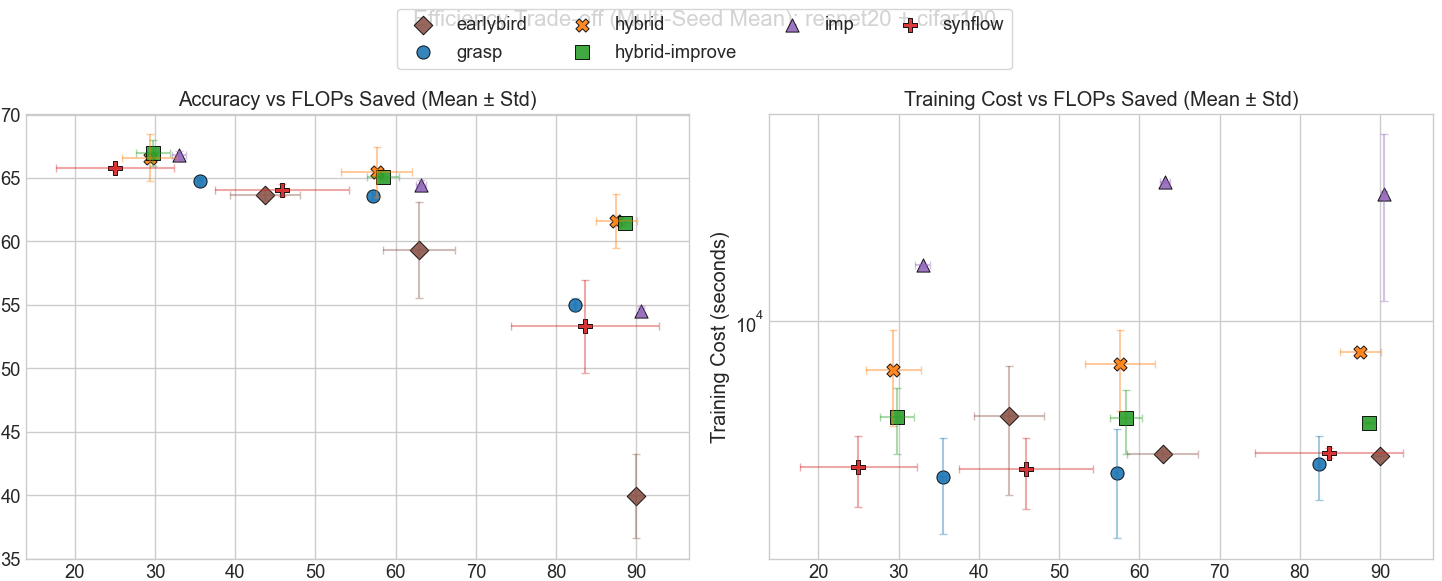
\includegraphics[width=\textwidth]{resnet20-cifar100_pareto.png}
	\caption{Biểu đồ Pareto: Cân bằng giữa độ chính xác và độ trễ trên CIFAR-100/ResNet-20}
	\label{fig:resnet20-cifar100-pareto}
\end{figure}
 
Hình~\ref{fig:resnet20-cifar100-pareto} cho thấy bức tranh hiệu quả tương tự như CIFAR-10 nhưng
với dải độ chính xác thấp hơn ($35\%$--$67\%$ thay vì $75\%$--$91\%$).
 
Tại tỉ lệ giảm FLOPs cao ($>80\%$), Hybrid và Hybrid-Improve đạt $\approx61{,}5\%$ độ chính
xác với chi phí huấn luyện trung bình, trong khi GraSP đạt $\approx55\%$ với chi phí thấp
hơn đáng kể.
IMP đạt $\approx54{,}5\%$ với chi phí rất cao --- càng khẳng định rằng chi phí
cao của IMP không tương xứng với hiệu suất ở mức độ thưa cực cao.
SynFlow đạt $\approx53\%$ với chi phí thấp, nhưng với độ biến động cao hơn.

\section{CIFAR-10/ResNet-50}

\subsection{Độ chính xác và sụt giảm theo mức độ thưa}
\label{subsec:r50_acc}
\begin{figure}
	\centering
	\begin{subfigure}{0.49\textwidth}
		\centering
		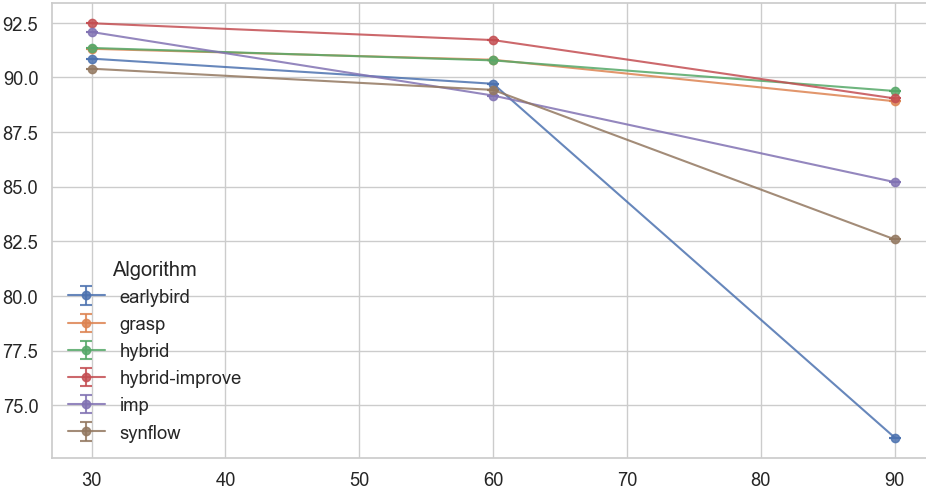
\includegraphics[width=\textwidth]{resnet50-cifar10_acc+sparsity.png}
		\caption{Độ chính xác theo mức độ thưa trên CIFAR-10/ResNet-50}
		\label{fig:resnet50-cifar10-acc-sparsity}
	\end{subfigure}
	\hfill
	\begin{subfigure}{0.49\textwidth}
		\centering
		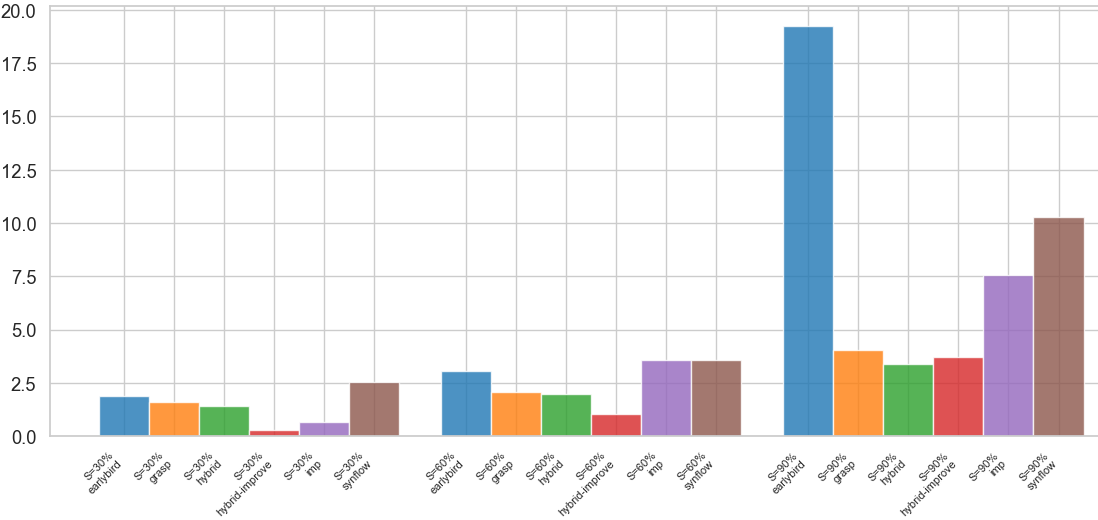
\includegraphics[width=\textwidth]{resnet50-cifar10_accdrop.png}
		\caption{Mức giảm độ chính xác so với mô hình dày đặc trên CIFAR-10/ResNet-50}
		\label{fig:resnet50-cifar10-accdrop}
	\end{subfigure}

	\caption{Độ chính xác theo mức độ thưa trên CIFAR-10/ResNet-50}
	\label{fig:grouped-accuracy}
\end{figure}
 
Hình~\ref{fig:resnet50-cifar10-acc-sparsity} và \ref{fig:resnet50-cifar10-accdrop} cho thấy các hiện tượng sau:

Sụt giảm âm $\approx-0{,}3\%$ của Hybrid-Improve tại $S=0{,}30$ không phải là sai số
đo lường --- đây là hiệu ứng điều chỉnh ngầm trong vùng dư thừa tham số, nơi cắt tỉa
nhẹ loại bỏ nhiễu và cải thiện khả năng tổng quát hóa.
Hybrid cũng đạt sụt giảm thấp ($\approx1{,}4\%$).
 
Hybrid-Improve tiếp tục dẫn đầu ($\approx1\%$ sụt giảm), tiếp theo là Hybrid
($\approx2\%$), GraSP ($\approx2\%$), Early-Bird ($\approx3\%$), IMP ($\approx3{,}5\%$)
và SynFlow ($\approx3{,}5\%$).
Sự nhất quán qua các kiến trúc củng cố kết luận rằng chiến lược hybrid mạnh mẽ ở mức nén
vừa phải bất kể độ sâu mạng.
 
Sụt giảm của IMP tăng từ $\approx5\%$ trên ResNet-20 lên $\approx7{,}5\%$ trên ResNet-50,
trong khi cấu hình ($10$ vòng lặp, $160$ epoch/vòng) không được tinh chỉnh lại.
Trên ResNet-50 ($\approx25$M tham số), $10$ vòng lặp phải xử lý không gian trọng số phức
tạp hơn nhiều, và điều kiện ổn định cần thiết cho cơ chế rewind khó đạt được hơn trong
cùng số epoch.
 
Sụt giảm của SynFlow tăng từ $\approx6{,}2\%$ trên ResNet-20 lên $\approx10{,}5\%$ ---
mức tăng lớn nhất trong tất cả các thuật toán không phải Early-Bird.
Như được ghi nhận trong bản đồ nhiệt (Hình~\ref{fig:r50_heatmap_s09}), tại $S=0{,}90$
nhiều tầng shortcut đạt $\approx100\%$ độ thưa, loại bỏ hiệu quả các kết nối residual và
biến ResNet-50 thành một mạng phẳng bị hư hại nghiêm trọng.
ResNet-50 có nhiều bottleneck block hơn gấp ba lần ResNet-20, mỗi block có một shortcut
chiếu $1{\times}1$, làm trầm trọng thêm xu hướng của SynFlow khi tập trung độ thưa vào các
kết nối này.
 
Hybrid đạt $\approx3{,}3\%$ sụt giảm độ chính xác tại $S=0{,}90$ trên ResNet-50 --- tốt hơn so với
ResNet-20.
Hybrid-Improve đạt $\approx3{,}5\%$ --- hầu như không đổi so với ResNet-20.
Sự ổn định giữa các kiến trúc này là kết quả quan trọng: chiến lược cắt tỉa của 2 thuật toán này không  
có bước reset weight như IMP (cũng sử dụng magnitude như tiêu chí cắt tỉa) cho phép mạng thích nghi dần
thay vì phải học lại từ đầu sau mỗi vòng như IMP.

Early-Bird sụt giảm ~19\% trên ResNet-50, tệ hơn so với ~17\% trên ResNet-20,
mặc dù ResNet-50 có kênh rộng hơn cung cấp nhiều
dư địa hơn trước. Hành vi sụp đổ vẫn xảy ra do điểm $\gamma$ BN tại giai đoạn sớm 
không đủ tin cậy ở $S=0{,}90$.
 
\subsection{Phân phối độ thưa theo tầng và tính ổn định}
\label{subsec:r50_layerwise}

\begin{figure}[h]
	\centering
	\begin{subfigure}{0.49\textwidth}
		\centering
		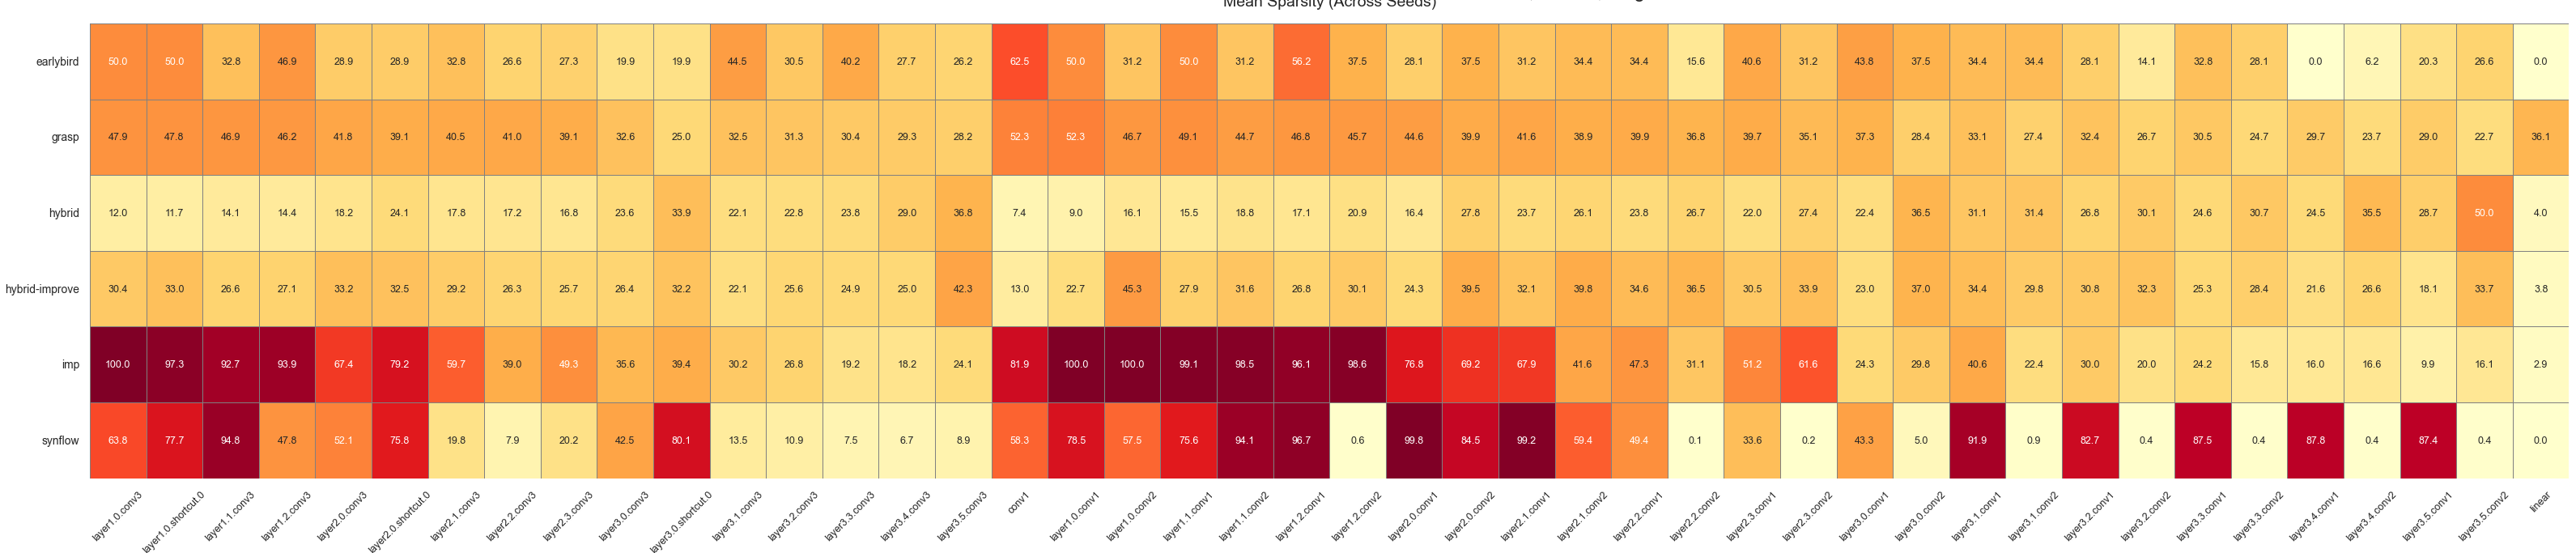
\includegraphics[width=\textwidth]{resnet50-cifar10_s0.3_heatmap.png}
		\caption{Bản đồ nhiệt phân phối độ thưa theo tầng tại $S=0{,}30$}
		\label{fig:r50_heatmap_s03}
	\end{subfigure}
	\hfill
	\begin{subfigure}{0.49\textwidth}
		\centering
		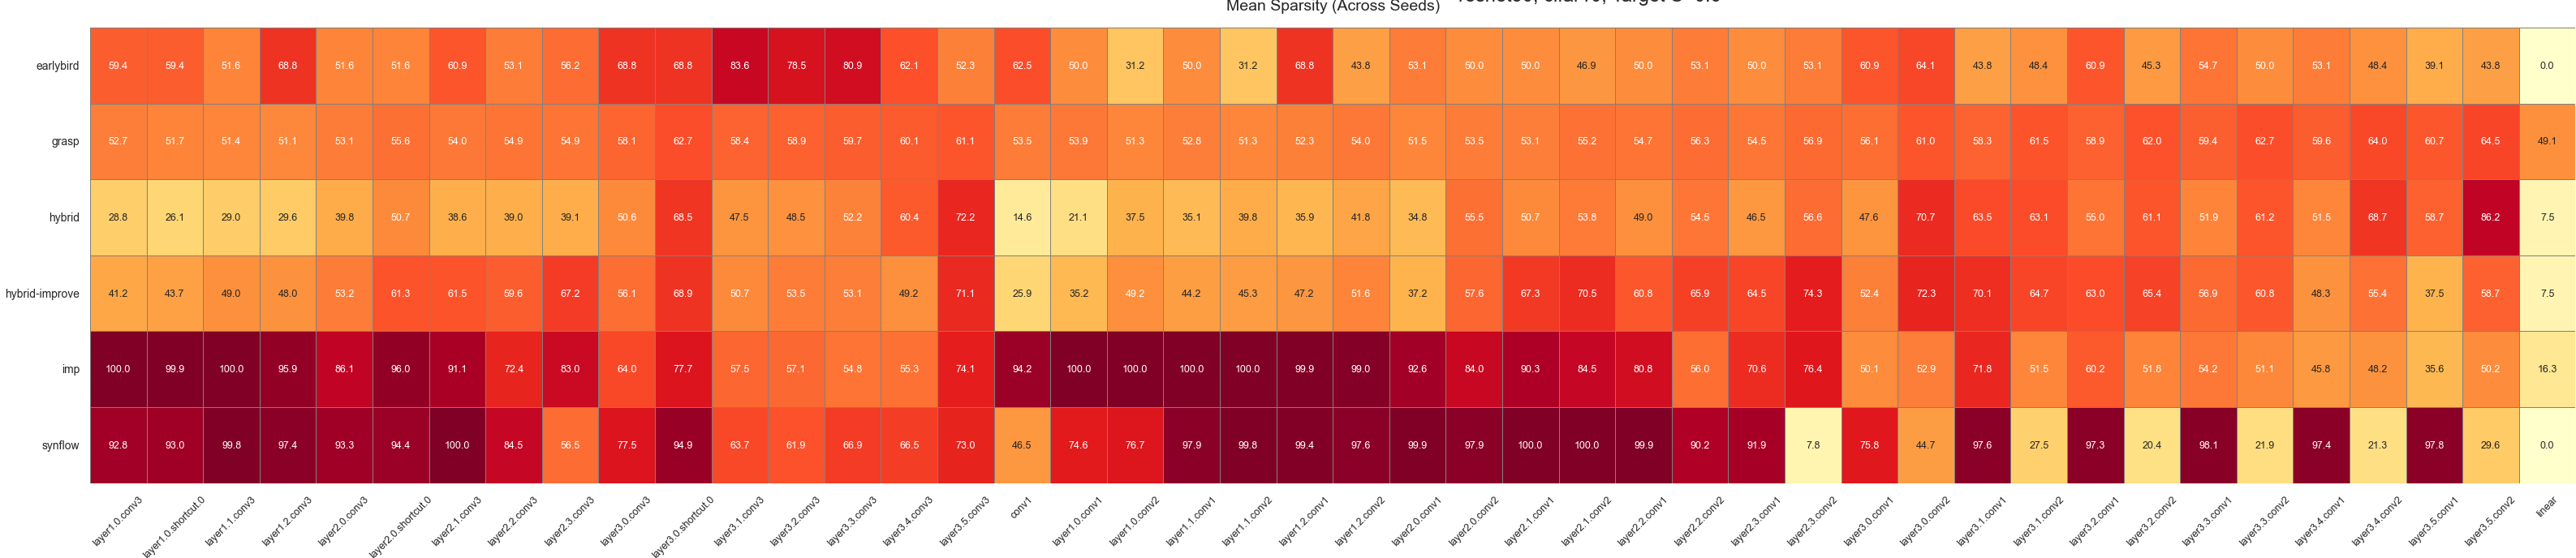
\includegraphics[width=\textwidth]{resnet50-cifar10_s0.6_heatmap.png}
		\caption{Bản đồ nhiệt phân phối độ thưa theo tầng tại $S=0{,}60$}
		\label{fig:r50_heatmap_s06}
	\end{subfigure}
	\hfill
	\begin{subfigure}{0.49\textwidth}
		\centering
		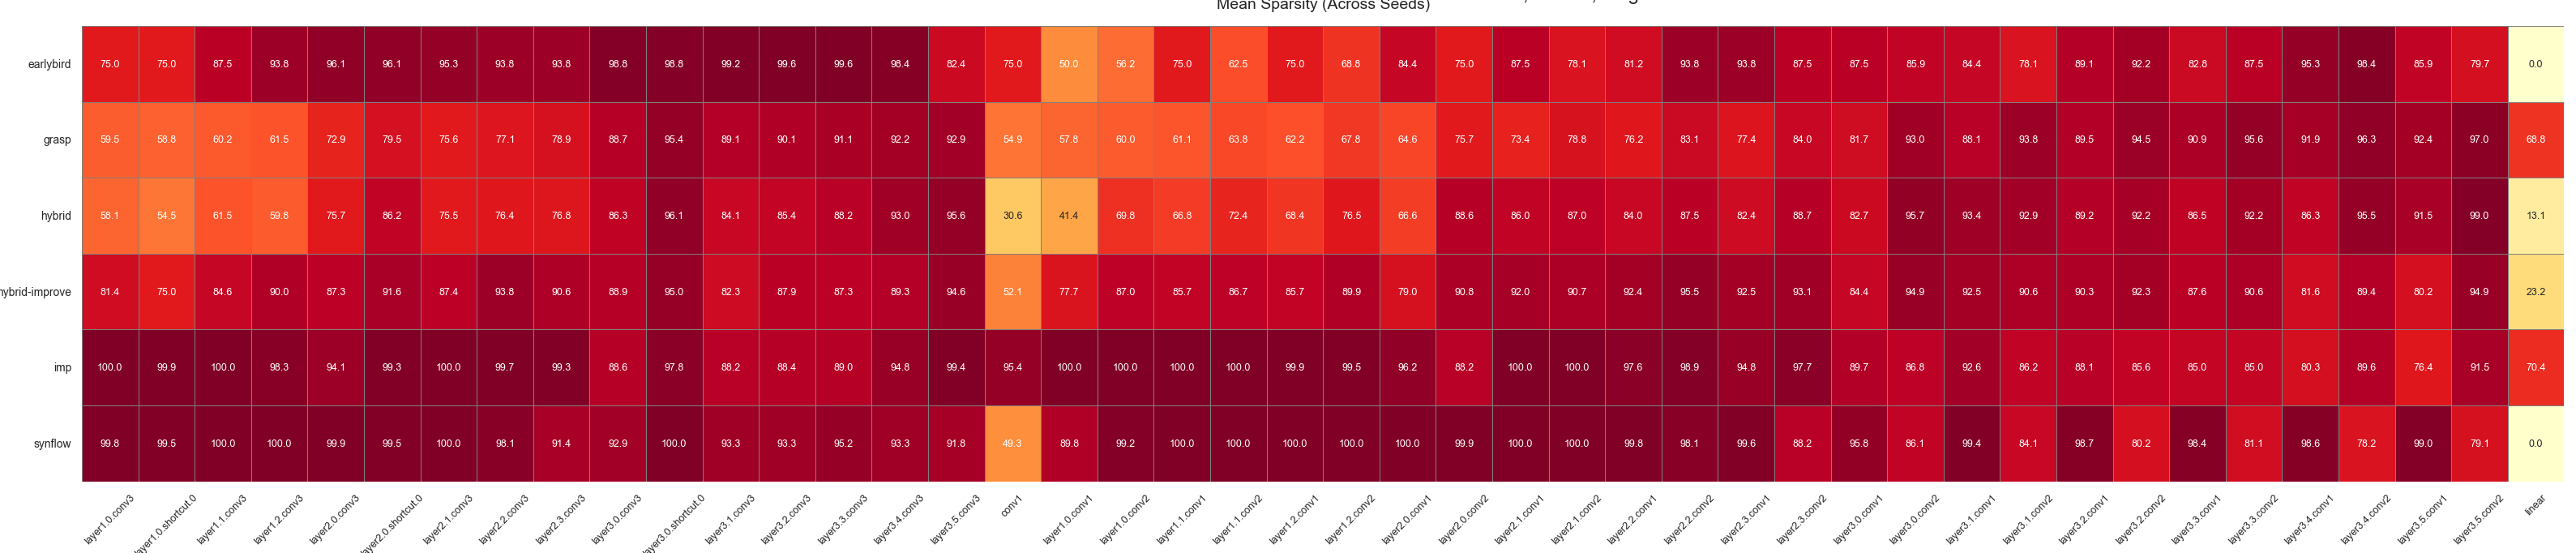
\includegraphics[width=\textwidth]{resnet50-cifar10_s0.9_heatmap.png}
		\caption{Bản đồ nhiệt phân phối độ thưa theo tầng tại $S=0{,}90$}
		\label{fig:r50_heatmap_s09}
	\end{subfigure}

	\caption{Bản đồ nhiệt phân phối độ thưa theo tầng trên CIFAR-10/ResNet-50}
	\label{fig:grouped-accuracy}
\end{figure}
 
Hình~\ref{fig:r50_heatmap_s03}, \ref{fig:r50_heatmap_s06} và \ref{fig:r50_heatmap_s09}
cho thấy các mô hình định tính tương tự như ResNet-20 nhưng với sự khác biệt về cường độ.
 
IMP trên ResNet-50 tại $S=0{,}30$ đã đẩy một số tầng shortcut đầu lên gần $100\%$ độ thưa
ngay cả ở $S=0{,}30$ --- cực đoan hơn nhiều so với ResNet-20 ở cùng mức nén.
Trong kiến trúc bottleneck, các tầng này chủ yếu đảm nhiệm vai trò mở rộng số chiều kênh và 
biến đổi biểu diễn đặc trưng. Trên CIFAR-10, mức độ mở rộng này có thể dư thừa so với độ phức 
tạp của bài toán, dẫn đến nhiều trọng số có độ lớn nhỏ và dễ bị loại bỏ.
 
GraSP tiếp tục là phương pháp phân phối đồng đều nhất, duy trì mức độ thưa tương đương
qua tất cả các tầng ngay cả trong kiến trúc sâu hơn, phản ánh rằng tiêu chí bảo toàn
gradient tìm kiếm sự đồng đều về đóng góp saliency mà không bị ảnh hưởng bởi sự khác
biệt về kích thước tầng.
 
SynFlow tại $S=0{,}90$ cho thấy nhiều tầng shortcut đạt $\approx99\%$--$100\%$ độ thưa,
xác nhận giả thuyết sụp đổ cấu trúc tại kết nối residual.


\subsection{Mức giảm FLOPs vs chi phí huấn luyện và độ chính xác}
Kết quả trên ResNet-50 có một số điểm khác biệt quan trọng so
với ResNet-20.

\begin{figure}
	\centering
	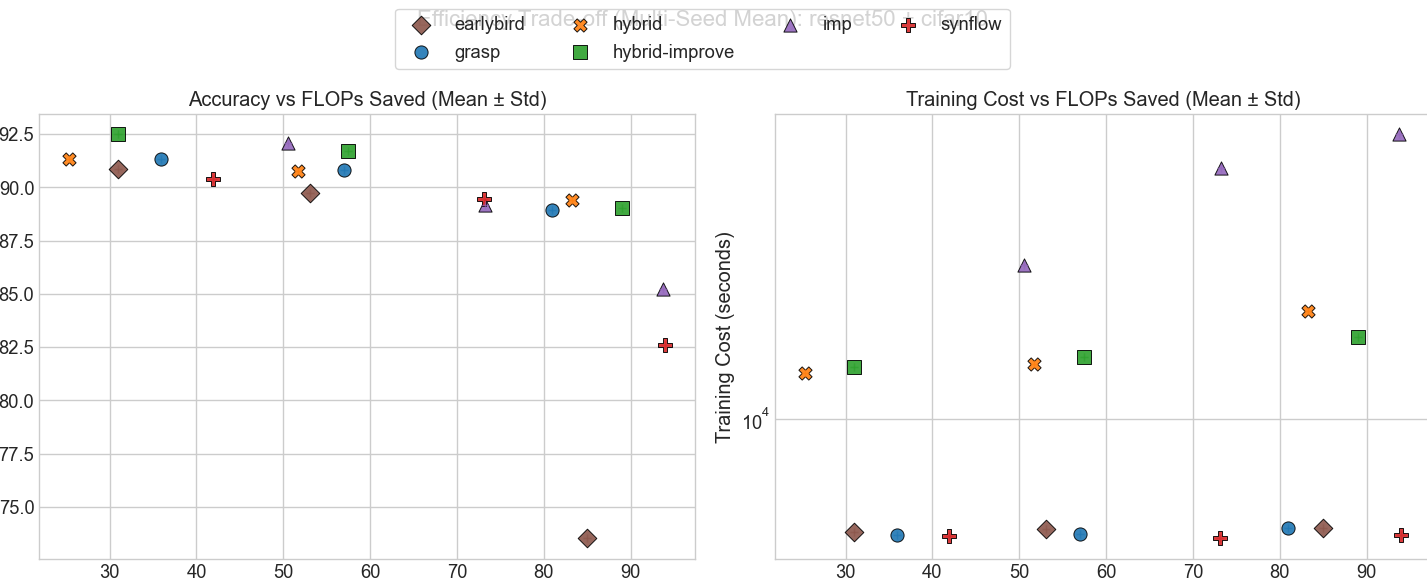
\includegraphics[width=\textwidth]{resnet50-cifar10_pareto.png}
	\caption{Biểu đồ Pareto: Cân bằng giữa độ chính xác và độ trễ trên CIFAR-10/ResNet-50}
	\label{fig:resnet50-cifar10-pareto}
\end{figure}

Tại $S=0{,}90$ ($\approx85\%$--$90\%$ FLOPs tiết kiệm), GraSP đạt $\approx89\%$
độ chính xác --- xấp xỉ bằng Hybrid ($\approx89{,}7\%$) và Hybrid-Improve
($\approx89{,}2\%$) --- nhưng với chi phí huấn luyện thấp hơn khoảng một bậc
độ lớn.
Trên ResNet-20, khoảng cách accuracy giữa GraSP và các biến thể hybrid tại
$S=0{,}90$ là $\approx2$--$3$ điểm phần trăm, đủ để biện minh cho chi phí cao
hơn của hybrid.
Trên ResNet-50, khoảng cách này thu hẹp xuống dưới $1$ điểm phần trăm, trong
khi chi phí huấn luyện vẫn chênh lệch lớn.
Điều này có nghĩa là trên ResNet-50/CIFAR-10, GraSP chiếm \emph{vị trí tốt hơn
trên biên Pareto} so với Hybrid và Hybrid-Improve khi xét đồng thời cả accuracy
lẫn chi phí huấn luyện.

Lý giải cho sự cải thiện tương đối này của GraSP trên ResNet-50 nằm ở đặc tính
bảo toàn chuẩn gradient của nó: với mạng sâu hơn và nhiều tham số hơn, tiêu chí
Hessian-gradient product của GraSP tạo ra phân phối độ thưa đồng đều hơn giữa
các tầng, tránh được các nút thắt cổ chai mà magnitude pruning toàn cục (IMP,
Hybrid) dễ tạo ra khi không gian trọng số lớn hơn nhiều \cite{grasp}.
 
% ===========================================================================
\section{Độ trễ suy diễn}
\label{sec:latency}
% ===========================================================================
\begin{figure}
	\centering
	\begin{subfigure}{0.49\textwidth}
		\centering
		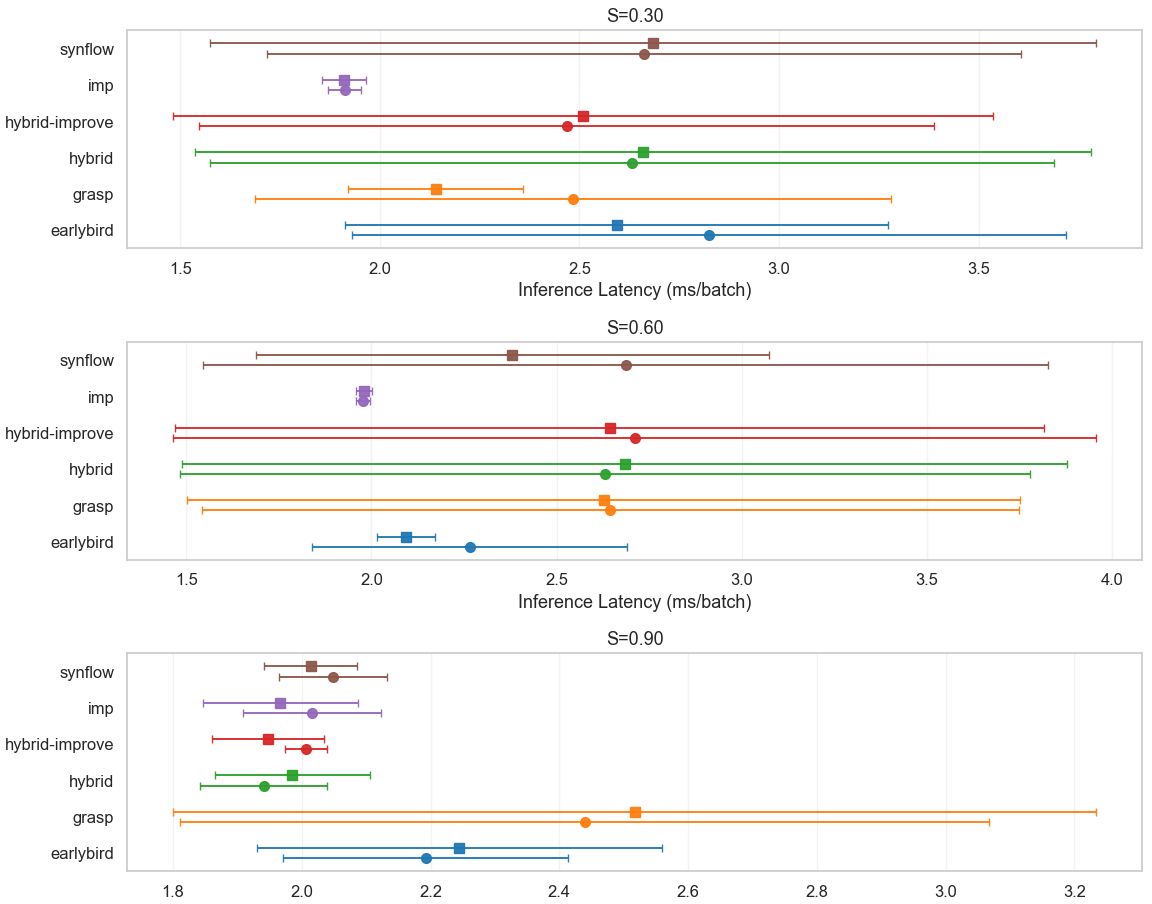
\includegraphics[width=\textwidth]{resnet20-cifar10_latency.png}
		\caption{Độ trễ suy diễn trên CIFAR-10/ResNet-20}
		\label{fig:r20c10_latency}
	\end{subfigure}
	\hfill
	\begin{subfigure}{0.49\textwidth}
		\centering
		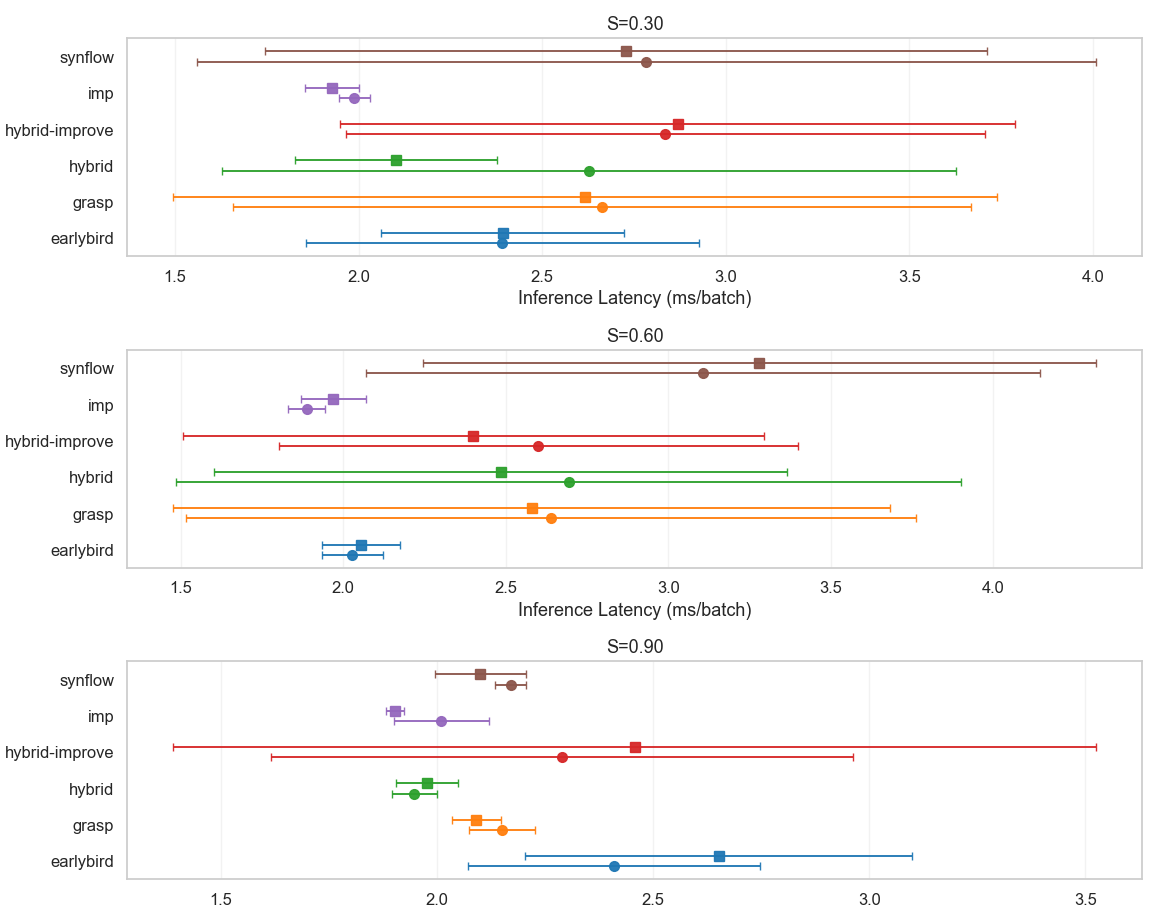
\includegraphics[width=\textwidth]{resnet20-cifar100_latency.png}
		\caption{Độ trễ suy diễn trên CIFAR-100/ResNet-20}
		\label{fig:r20c100_latency}
	\end{subfigure}
	\hfill
	\begin{subfigure}{0.49\textwidth}
		\centering
		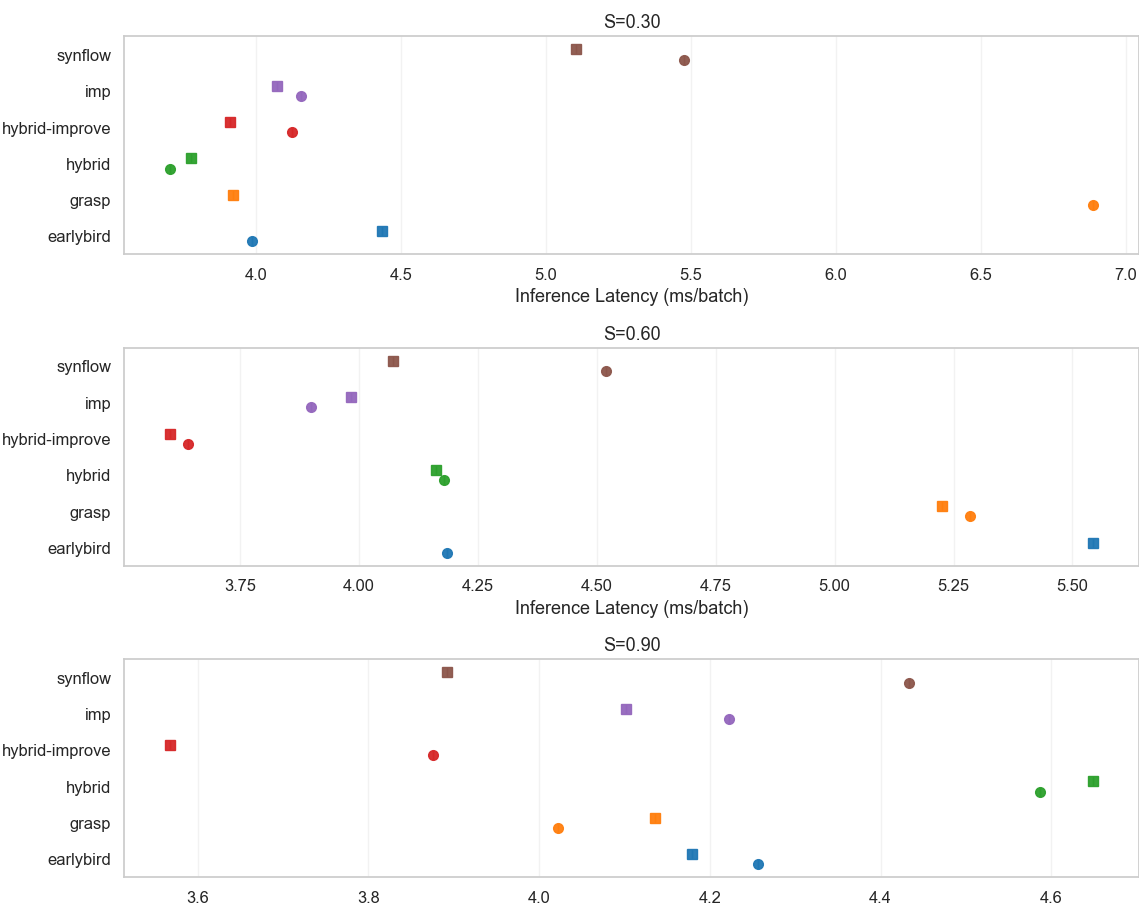
\includegraphics[width=\textwidth]{resnet50-cifar10_latency.png}
		\caption{Độ trễ suy diễn trên CIFAR-10/ResNet-50}
		\label{fig:r50_latency}
	\end{subfigure}

	\caption{So sánh độ trễ suy diễn giữa mô hình gốc và mô hình đã cắt tỉa trên các cấu hình khác nhau}
	\label{fig:grouped-accuracy}
\end{figure}
 
Hình~\ref{fig:r20c10_latency}, \ref{fig:r20c100_latency} và \ref{fig:r50_latency} trình
bày so sánh độ trễ suy diễn (ms/batch) giữa mô hình gốc (hình tròn) và mô hình đã cắt tỉa
(hình vuông) cho mỗi thuật toán và mức độ thưa.
Quan sát nổi bật nhất là tất cả các
phương pháp không có cấu trúc đều có thanh lỗi rất lớn về độ trễ, đặc biệt ở mức độ thưa
thấp và vừa.
Tại $S=0{,}30$ và $S=0{,}60$ trên ResNet-20, thanh lỗi của nhiều thuật toán (SynFlow,
Hybrid, Hybrid-Improve, GraSP, Early-Bird) trải rộng hơn $2$ ms --- gần bằng toàn bộ dải
giá trị đo được.
Điều này có nghĩa là sự khác biệt quan sát được giữa mô hình gốc và mô hình đã cắt tỉa
nằm hoàn toàn trong vùng nhiễu đo lường.
Đến $S=0{,}90$, các thanh lỗi thu hẹp đáng kể (khoảng $\pm0{,}1$--$0{,}3$ ms), nhưng
lúc này sự khác biệt giữa dense và pruned cũng biến mất --- mọi thuật toán tập trung trong
khoảng $1{,}8$--$2{,}6$ ms/batch với ResNet-20.



\chapter{Kết luận}
Luận văn này đã thực hiện khảo sát và đánh giá thực nghiệm nhiều thuật toán cắt tỉa mạng nơ-ron,
bao gồm GraSP, SynFlow, IMP, Early-Bird, Hybrid và Hybrid-Improve,
trên các cấu hình ResNet-20/CIFAR-10, ResNet-20/CIFAR-100 và ResNet-50/CIFAR-10.

Kết quả cho thấy các phương pháp hybrid đạt cân bằng tốt nhất giữa độ chính xác,
chi phí huấn luyện và tính ổn định.
Hybrid và Hybrid-Improve duy trì mức sụt giảm tương đối nhỏ ngay cả ở $90\%$ sparsity,
đồng thời ổn định hơn đáng kể so với các phương pháp khác.
Trong đó, Hybrid-Improve cho thấy độ ổn định tốt nhất giữa các lần chạy khác nhau.

GraSP nổi bật ở khả năng tạo phân phối độ thưa đồng đều và ổn định giữa các tầng,
trong khi SynFlow cho thấy độ nhạy cao với khởi tạo ngẫu nhiên.
IMP đạt hiệu suất tương đối tốt nhưng chi phí huấn luyện rất cao,
làm hạn chế tính thực tiễn ở quy mô lớn.
Early-Bird là phương pháp kém ổn định nhất tại mức độ thưa cực cao,
đặc biệt trên CIFAR-100.

Nhìn chung, kết quả thực nghiệm xác nhận rằng không tồn tại một thuật toán pruning tối ưu cho mọi trường hợp.
Hiệu quả của pruning phụ thuộc mạnh vào kiến trúc mạng, độ khó của bài toán,
mức độ thưa mục tiêu và năng lực tính toán của phần cứng.
Tuy nhiên, các chiến lược hybrid cho thấy tiềm năng lớn như một hướng tiếp cận cân bằng
giữa hiệu suất và chi phí, đặc biệt trong các bài toán yêu cầu mức nén cao nhưng vẫn cần duy trì độ chính xác.

%\rhead{\thepage}  % Sets the right side header to show the page number
%\lhead{}  % Clears the left side page header
% \renewcommand{\footrulewidth}{0.4pt}  % not defined for scrlayer-scrpage; commented out

\bibliographystyle{plain} % ieeetr
\bibliography{refs} 

\end{document}
